%%
%% (
%%  )\ )                             (
%%  (()/(   (            (             )\  )   (
%%   /(_))  ))\   (       ))\  (   (   (()/(   ))\
%%   (_))  /((_)  )\  )  /((_) )\  )\   ((_))/((_)
%%   | _ \(_))(  _(_/( (_) )  ((_)((_)  _| |(_))
%%   |   /| || || ' \))/ -_)/ _|/ _ \/ _` |/ -_)
%%   |_|_\ \_,_||_||_| \___|\__|\___/\__,_|\___|
%%

\documentclass{article}
\usepackage{fontspec}
\usepackage[utf8]{inputenc}
\usepackage{amsmath}
%\usepackage{slashbox}
\usepackage{amsfonts}
\usepackage{amssymb}
\usepackage{graphicx} % Paquete para incluir imágenes en el documento LaTeX
\usepackage{hyperref}
\hypersetup{
  colorlinks=true,
  linkcolor=blue,
  filecolor=magenta,
  urlcolor=cyan,
}
\urlstyle{same}
\usepackage{varwidth}

\newcommand\tab[1][1cm]{\hspace*{#1}}

\usepackage{multirow}

\usepackage[a4paper,rmargin=1.5cm,lmargin=1.5cm,top=1.5cm,bottom=1.5cm]{geometry}

\usepackage{pdfpages}

\usepackage{xcolor}
\usepackage{minted}
\setminted[css]{frame=lines, framesep=2mm, baselinestretch=1.2, rulecolor=\color{black!80},
                bgcolor=DarkGray,fontsize=\normalsize}
\usemintedstyle[css]{monokai}
\setminted[python]{frame=lines, framesep=2mm, baselinestretch=1.2, rulecolor=\color{black!80}, bgcolor=DarkGray}
\usemintedstyle[python]{monokai}
\setminted[java]{frame=lines, framesep=2mm, baselinestretch=1.2, rulecolor=\color{black!80}, bgcolor=DarkGray}
\usemintedstyle[java]{monokai}
\setminted[javascript]{frame=lines, framesep=2mm, baselinestretch=1.2, rulecolor=\color{black!80}, bgcolor=DarkGray}
\usemintedstyle[javascript]{monokai}
\setminted[php]{frame=lines, framesep=2mm, baselinestretch=1.2, rulecolor=\color{black!30}, bgcolor=LightGray}
\setminted[html]{frame=lines, framesep=2mm, baselinestretch=1.2, rulecolor=\color{black!30}, bgcolor=LightGray}
\setminted[bash]{baselinestretch=1.2,rulecolor=\color{black!30},bgcolor=LightGray}
\definecolor{LightGray}{gray}{0.98}
\definecolor{DarkGray}{gray}{0.1}
\definecolor{MidGray}{gray}{0.8}
\definecolor{codegreen}{rgb}{0,0.6,0}
\definecolor{codegray}{rgb}{0.5,0.5,0.5}
\definecolor{codepurple}{rgb}{0.58,0,0.82}
\definecolor{backcolour}{rgb}{0.95,0.95,0.92}
\setminted[json]{frame=lines, framesep=2mm, baselinestretch=1.2, rulecolor=\color{black!80}, bgcolor=DarkGray}
\usemintedstyle[json]{monokai}
\setminted[apacheconf]{frame=lines, framesep=2mm, baselinestretch=1.2, rulecolor=\color{black!30}, bgcolor=LightGray}
\setminted[html+twig]{frame=lines, framesep=2mm, baselinestretch=1.2, rulecolor=\color{black!30}, bgcolor=LightGray}
\setminted[html+php]{frame=lines, framesep=2mm, baselinestretch=1.2, rulecolor=\color{black!30}, bgcolor=LightGray}

%\setlength{\parindent}{0px}  % Setea la indentacion de la primera linea de cada parrafo a cero pixeles.


\title{Introducción a JavaSE}
\author{@RuneCode}

\begin{document}
%% Portada
%%\includepdf{./portada/portada.pdf}

%% Clase 1
\section{Presentacion del curso}%
Bienvenido al \textbf{Curso de Introducción a PHP} en este curso el profesor
Héctor Benitez, @HectorBenitez en Twitter, te irá enseñando los fundamentos de
PHP mientras desarrollas un proyecto que servirá de sitio web personal.\\

En este curso veremos:
\begin{itemize}
  \item Programación orientada a Objetos.
  \item Conexión a bases de datos.
  \item Usaremos los estándares de PHP
  \item Implementaremos librerías de terceros.
  \item Estructuraremos nuestro proyecto de una forma muy profesional que te
    servirá para futuros proyectos.
  \item Utilizaremos la versión 7.2 de PHP
\end{itemize}

%% Clase 2
\section{¿Qué es PHP?}%
PHP es un lenguaje de programación de propósito general de alto nivel que fue
diseñado especialmente para el desarrollo de aplicaciones web.\\

Es interpretado, multiplataforma, open source, el cual ha sido muy popular en
los últimos años.\\

\begin{figure}[h!]
  \centering
  
\includegraphics[scale=0.5]{./Pictures/001_php_laravel_sf_wp.jpg}
\end{figure}


\textbf{¿Qué NO es PHP?}
\begin{itemize}
  \item No es un lenguaje compilado, por lo cual siempre tendrás que llevar
    juntos tu código y tu interprete.
  \item No esta diseñado para realizar aplicaciones de escritorio.
\end{itemize}

Para trabajar con PHP instalaremos un entorno de desarrollo llamado devilbox, no
es un entorno pensado para producción.\\

\newpage

%% Clase 3
\section{Setup y Herramientas}% 
% En esta sección vamos a instalar XAMPP (x porque es multiplataforma, A porque
% tiene Apache, M de MariaDB, P de PHP y P de perl)\\
%
% Vamos a descargar XAMPP desde el siguiente
% \href{https://www.apachefriends.org/es/index.html}{enlace}.\\
%
% \begin{figure}[h!]
%     \centering
%       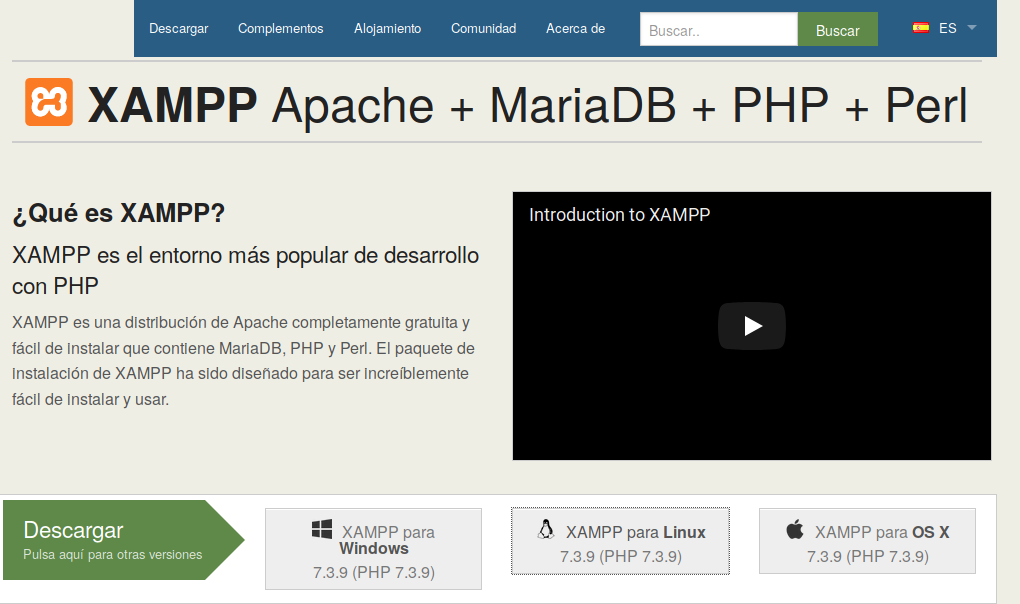
\includegraphics[scale=0.5]{./Pictures/001_ins.png}
% \end{figure}
%
% \begin{figure}[h!]
%     \centering
%       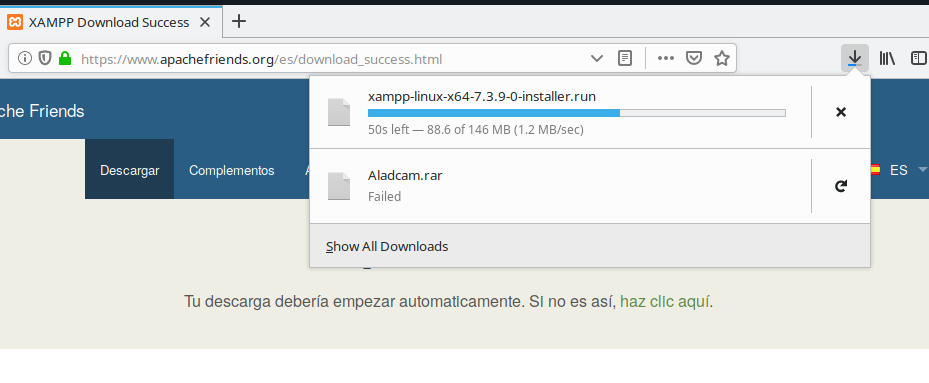
\includegraphics[scale=0.65]{./Pictures/001_ins_XAMPP.png}
% \end{figure}
%
% Para poder usar el instalador en Ubuntu primero damos permisos de ejecución al
% fichero descargado.\\
%
% \begin{minted}{bash}
%     chmod 755 xampp-linux-x64-7.3.9-0-installer.run
%       sudo ./xampp-linux-x64-7.3.9-0-installer.run
% \end{minted}
%
% \begin{figure}[h!]
%     \centering
%       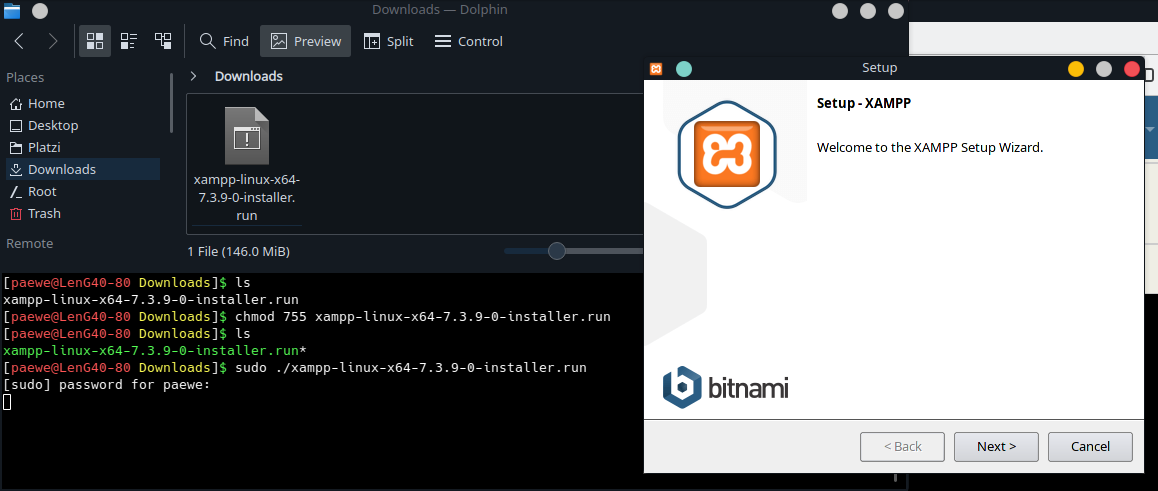
\includegraphics[scale=0.6]{./Pictures/002_instalar_XAMPP.png}
% \end{figure}
%
% \begin{figure}[h!]
%     \centering
%       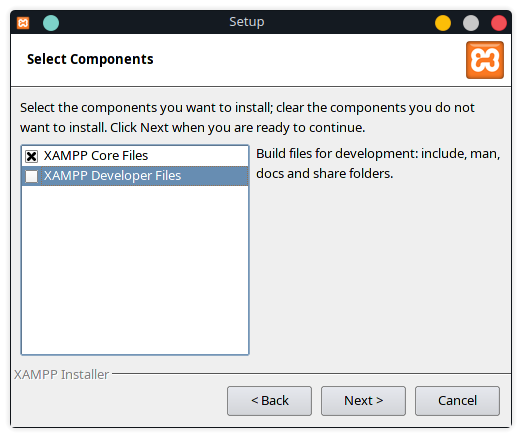
\includegraphics[scale=0.65]{./Pictures/003_components.png}
% \end{figure}
%
% \newpage
%
% \begin{figure}[h!]
%     \centering
%       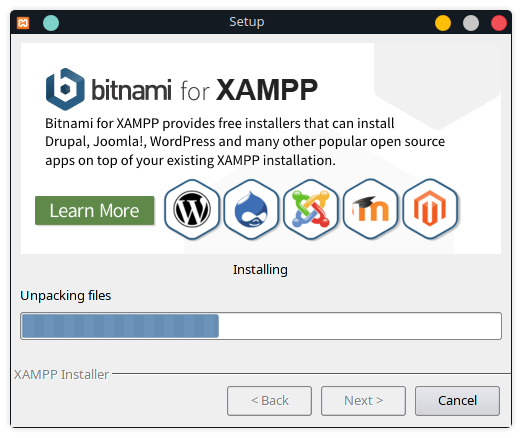
\includegraphics[scale=0.65]{./Pictures/003_instalar_XAMPP.png}
% \end{figure}
%
%
% \begin{figure}[h!]
%     \centering
%       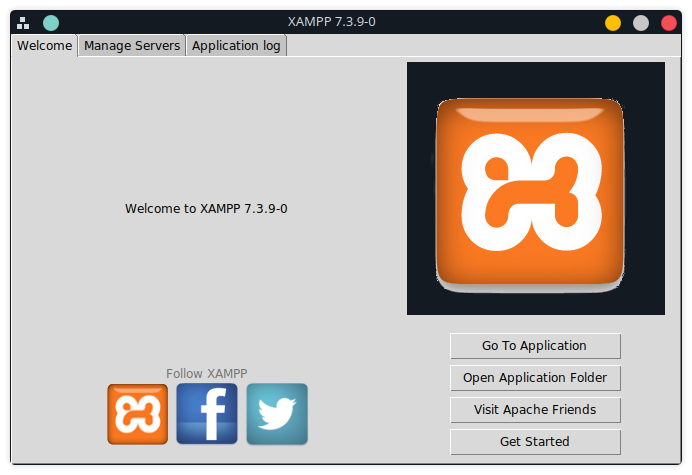
\includegraphics[scale=0.65]{./Pictures/004_XAMPP.png}
% \end{figure}
%
% \begin{figure}[h!]
%     \centering
%       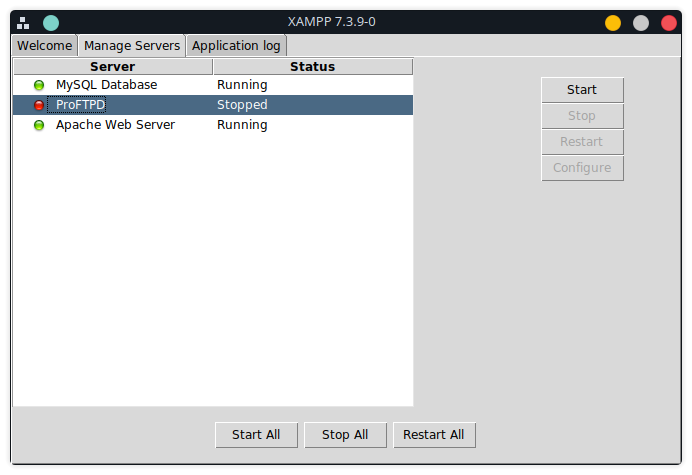
\includegraphics[scale=0.65]{./Pictures/005_servicios.png}
% \end{figure}
%
% \newpage
%
% \begin{figure}[h!]
%     \centering
%       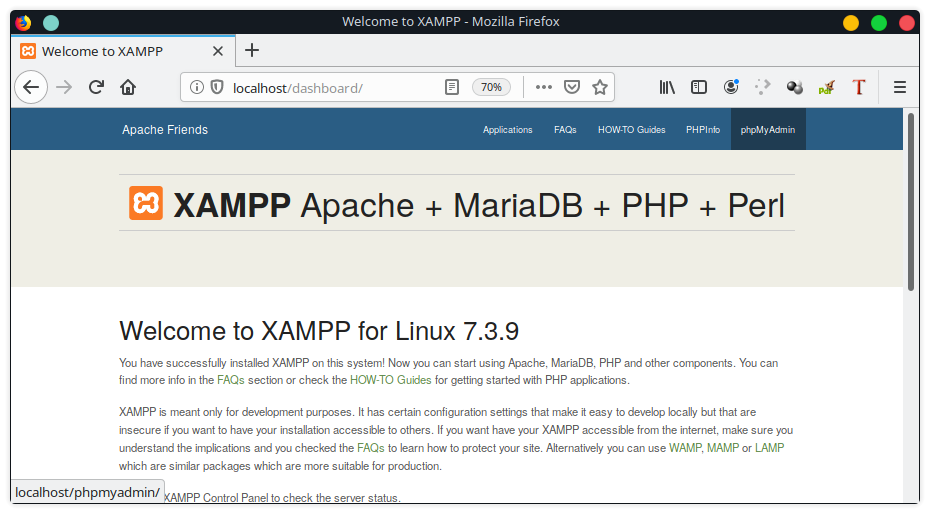
\includegraphics[scale=0.6]{./Pictures/006_localhost.png}
% \end{figure}
%
% \begin{figure}[h!]
%     \centering
%       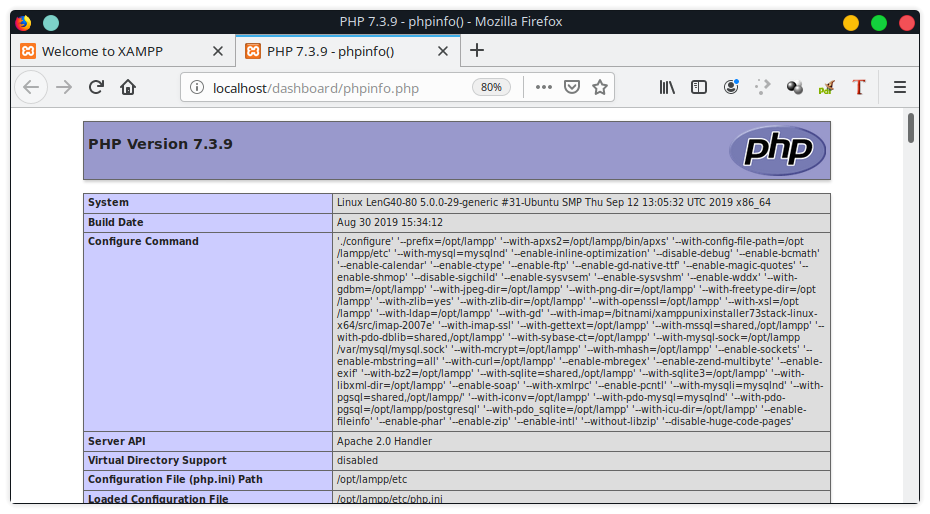
\includegraphics[scale=0.6]{./Pictures/007_php_info.png}
% \end{figure}
%
% \begin{figure}[h!]
%     \centering
%       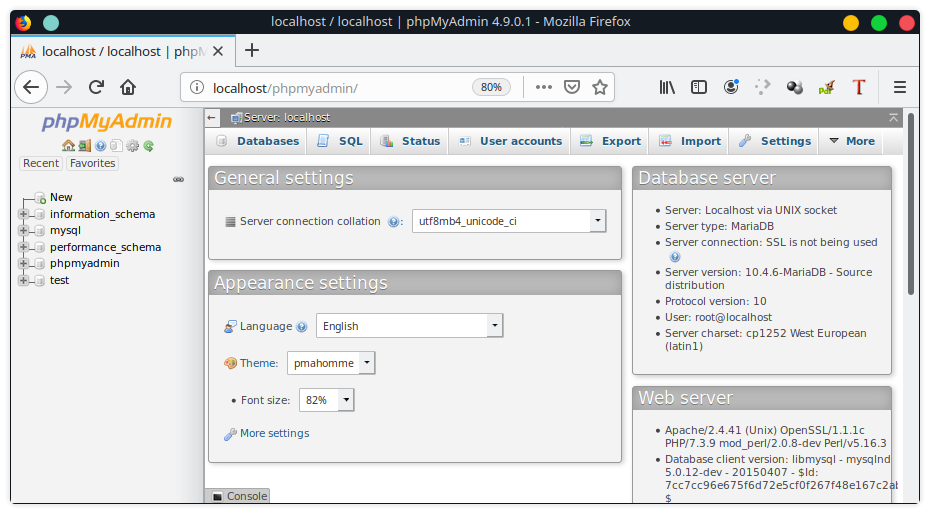
\includegraphics[scale=0.6]{./Pictures/008_phpMyAdmin.png}
% \end{figure}

\textbf{Devilbox, la caja mágica del desarrollo web en local}\\ Vamos a usar
\textbf{devilbox} que es un stack completo para la programación de aplicaciones
web. Aunque hereda del modelo con la base en PHP, permite instalar software de
todo tipo, ya que está basado en contenedores Docker. Esto nos brinda muchas
ventajas si queremos gestionar muchos proyectos.\\

Primero vamos a instalar \textbf{docker} en nuestro sistema operativo.\\
Para esto actualizamos los repositorios para instalar previamente algunos
paquetes necesarios.

\begin{minted}[fontsize=\footnotesize]{bash}
  sudo apt update
  sudo apt install apt-transport-https ca-certificates curl gnupg-agent software-properties-common
\end{minted}

\begin{figure}[h!]
  \centering
  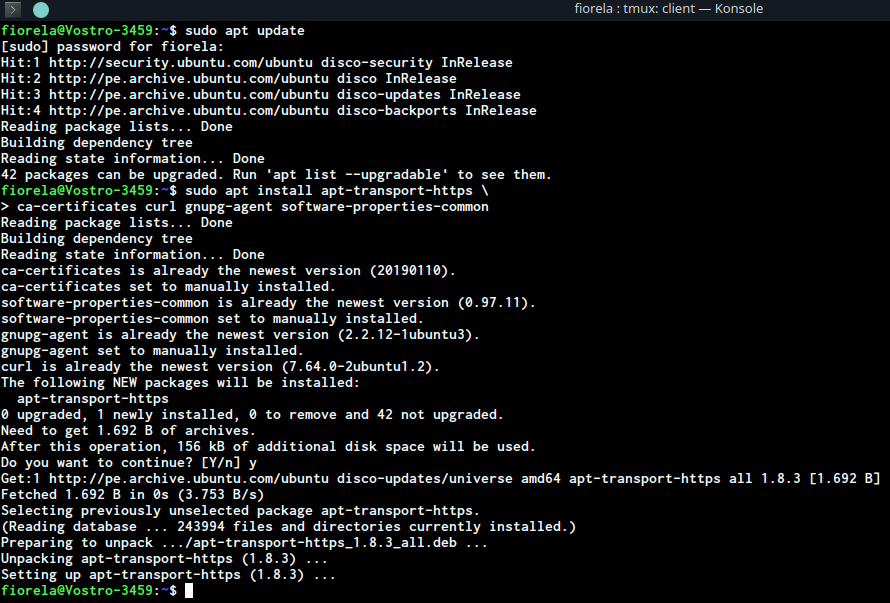
\includegraphics[scale=0.75]{./Pictures/Devilbox/001_docker.png}
\end{figure}

Luego descargamos la llave gpg usando curl.\\

\begin{minted}[fontsize=\footnotesize]{bash}
  curl -fsSL https://download.docker.com/linux/ubuntu/gpg | sudo apt-key add -
  sudo apt-key fingerprint 0EBFCD88
\end{minted}

\begin{figure}[h!]
  \centering
  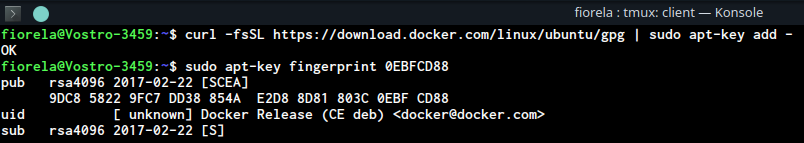
\includegraphics[scale=0.75]{./Pictures/Devilbox/002_docker.png}
\end{figure}

Ahora agregamos el repositorio.\\

\begin{minted}[fontsize=\footnotesize]{bash}
  sudo add-apt-repository "deb [arch=amd64] https://download.docker.com/linux/ubuntu $(lsb_release -cs) stable"
\end{minted}

\newpage

\begin{figure}[h!]
  \centering
  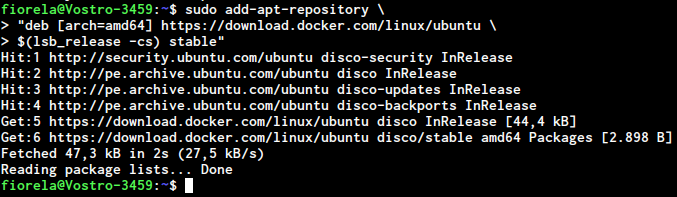
\includegraphics[scale=0.75]{./Pictures/Devilbox/003_docker.png}
\end{figure}

Actualizamos los repositorios nuevamente e instalamos docker:

\begin{minted}[fontsize=\footnotesize]{bash}
  sudo apt update
  sudo apt install docker-ce docker-ce-cli containerd.io
\end{minted}

\begin{figure}[h!]
  \centering
  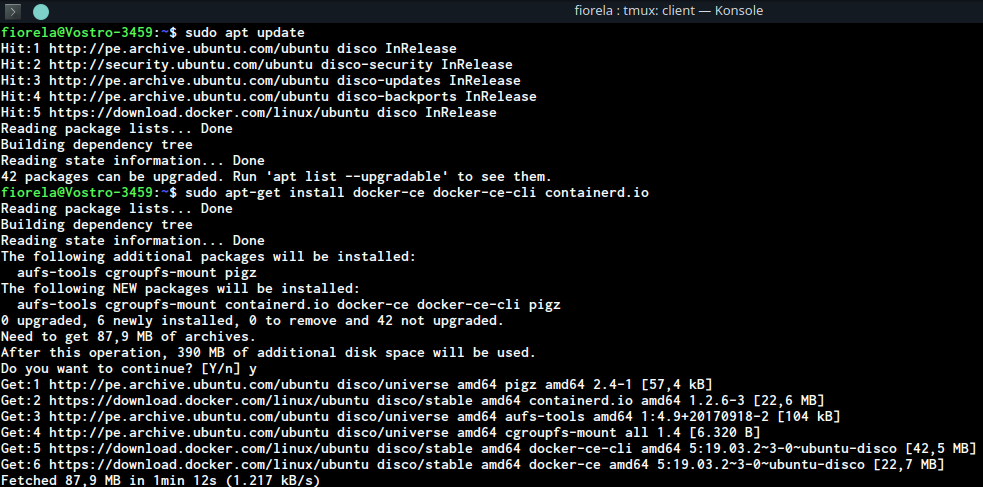
\includegraphics[scale=0.65]{./Pictures/Devilbox/004_docker.png}
\end{figure}

Podemos ejecutar docker como super usuario. Para probar que funciona podemos
hacer nuestro primer hello-world.

\begin{minted}[fontsize=\footnotesize]{bash}
  docker run hello-world
\end{minted}

\begin{figure}[h!]
  \centering
  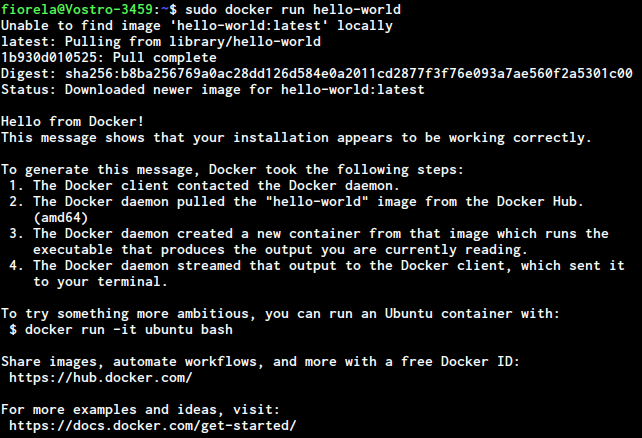
\includegraphics[scale=0.75]{./Pictures/Devilbox/005_docker.png}
\end{figure}

Para que puedas ejecutar docker sin ser un superusuario debes agregar tu user
al grupo \textbf{docker}. Ten en cuenta que puedes crear el grupo
\textbf{docker} en caso no se haya creado automáticamente.\\

\begin{minted}[fontsize=\footnotesize]{bash}
  sudo groupadd docker
  sudo usermod -aG docker $USER
  newgrp docker
  docker run hello-world
\end{minted}

Como se visualiza, ahora con nuestro usuario no es necesario correr docker
usando \textbf{sudo}.\\

\begin{figure}[h!]
  \centering
  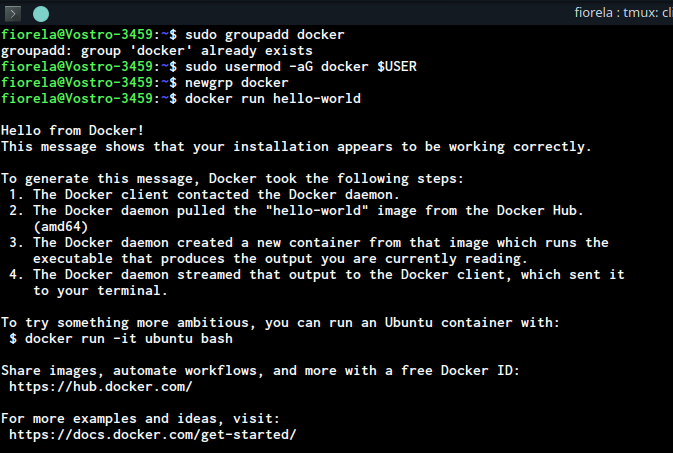
\includegraphics[scale=0.75]{./Pictures/Devilbox/006_docker_user.png}
\end{figure}

Ya que tenemos docker instalado ahora haremos clone del repositorio de
devilbox.\\

\begin{minted}[fontsize=\footnotesize]{bash}
  git clone https://github.com/cytopia/devilbox.git
  cd devilbox/
\end{minted}

\begin{figure}[h!]
  \centering
  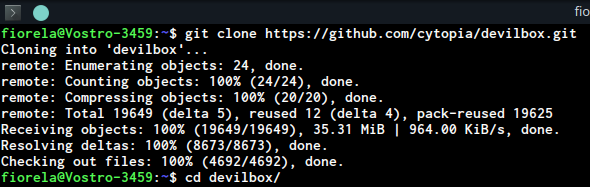
\includegraphics[scale=0.75]{./Pictures/Devilbox/007_devilbox.png}
\end{figure}

Dentro del repositorio que hemos clonado hay un fichero llamado
\textbf{env-example} que debemos copiar en un nuevo fichero
llamado \textbf{.env}, este será un fichero con el que podremos configurar
devilbox.\\

\begin{minted}{php}
  cp env-example .env
\end{minted}

\newpage

\begin{figure}[h!]
  \centering
  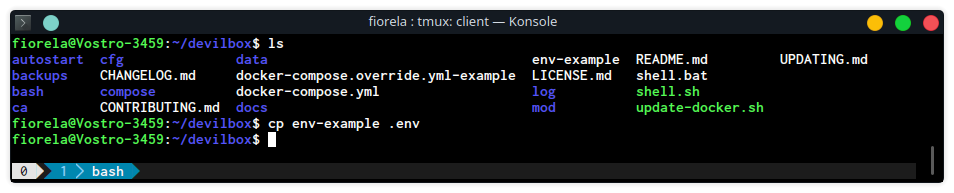
\includegraphics[scale=0.7]{./Pictures/Devilbox/008_devilbox.png}
\end{figure}

Vamos a empezar configurar en nuestro fichero \textbf{.env} el user id y
grupo id. Podemos saber nuestro uid y gid de la siguiente manera:

\begin{minted}[fontsize=\footnotesize]{bash}
  id -u
  id -g
\end{minted}

\begin{figure}[h!]
  \centering
  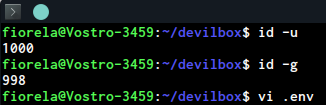
\includegraphics[scale=0.75]{./Pictures/Devilbox/011_devilbox.png}
\end{figure}

\begin{figure}[h!]
  \centering
  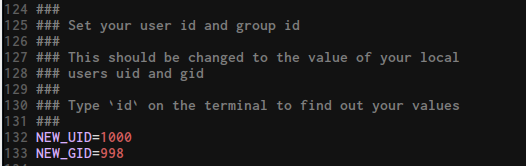
\includegraphics[scale=0.75]{./Pictures/Devilbox/012_devilbox.png}
\end{figure}

En el fichero \textbf{.env} también podemos elegir imagenes docker que deseamos
usar para nuestro entorno local de desarrollo.\\

\textbf{Base de datos}: En este caso descomentamos mysql-8.0\\

\begin{figure}[h!]
  \centering
  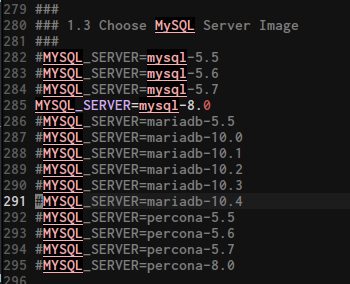
\includegraphics[scale=0.75]{./Pictures/Devilbox/009_devilbox_mysql8.png}
\end{figure}

Servidor HTTPD: Usaremos apache-2.4 ya que queremos montar el popular stack
\textbf{LAMP}.\\

\begin{figure}[h!]
  \centering
  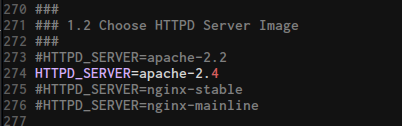
\includegraphics[scale=0.75]{./Pictures/Devilbox/010_devilbox_apache24.png}
\end{figure}

Php server: Usaremos la versión 7.2:\\

\begin{figure}[h!]
  \centering
  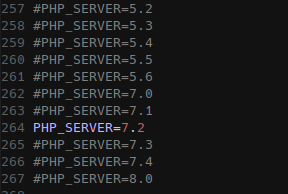
\includegraphics[scale=0.75]{./Pictures/011_php_server.png}
\end{figure}

Como se observa tenemos bastantes imágenes que podemos usar para nuestro
proyecto simplemente descomentandolas en el fichero \textbf{.env}.\\

Ahora para levantar nuestro entorno de desarrollo necesitamos instalar
\textbf{docker-compose}:

\begin{minted}[fontsize=\footnotesize]{bash}
  sudo apt install docker-compose
\end{minted}

\begin{figure}[h!]
  \centering
  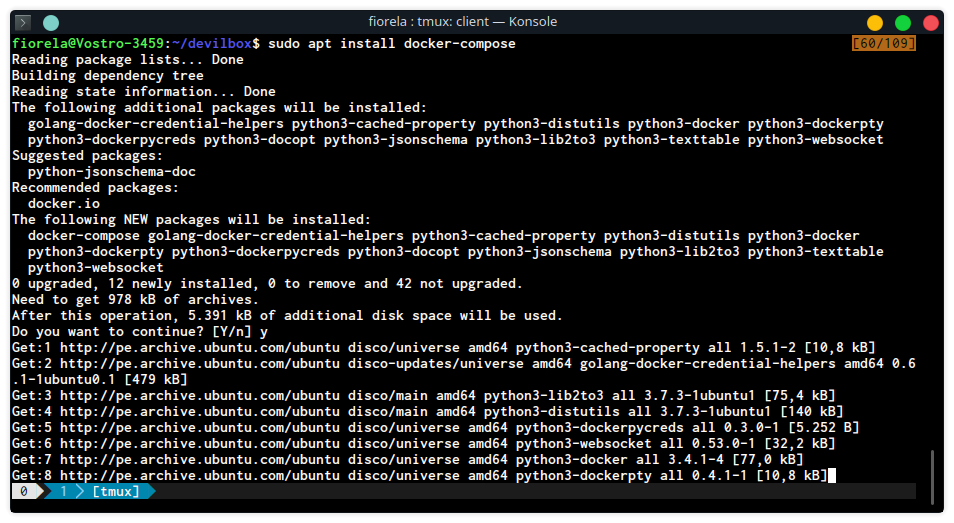
\includegraphics[scale=0.65]{./Pictures/Devilbox/013_docker_compose.png}
\end{figure}

Para levantar nuestro entorno con el servidor httpd php y mysql usamos el
siguiente comando:

\begin{minted}[fontsize=\footnotesize]{bash}
  docker-compose up httpd php mysql
\end{minted}

\begin{figure}[h!]
  \centering
  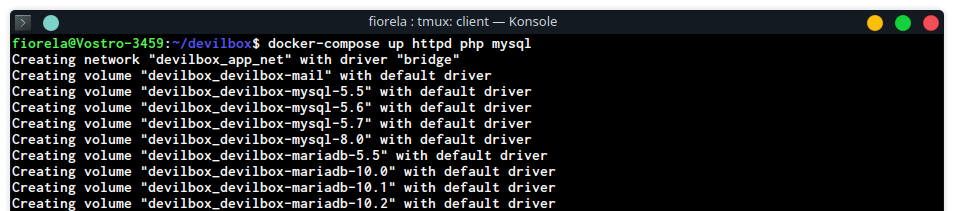
\includegraphics[scale=0.65]{./Pictures/Devilbox/014_compose_up.png}
\end{figure}

En caso que no tenga la imagen docker, entonces hará pull de las imágenes que
hemos descomentado en nuestro fichero \textbf{.env}. Esto demorará un poco.\\

\newpage

\begin{figure}[h!]
  \centering
  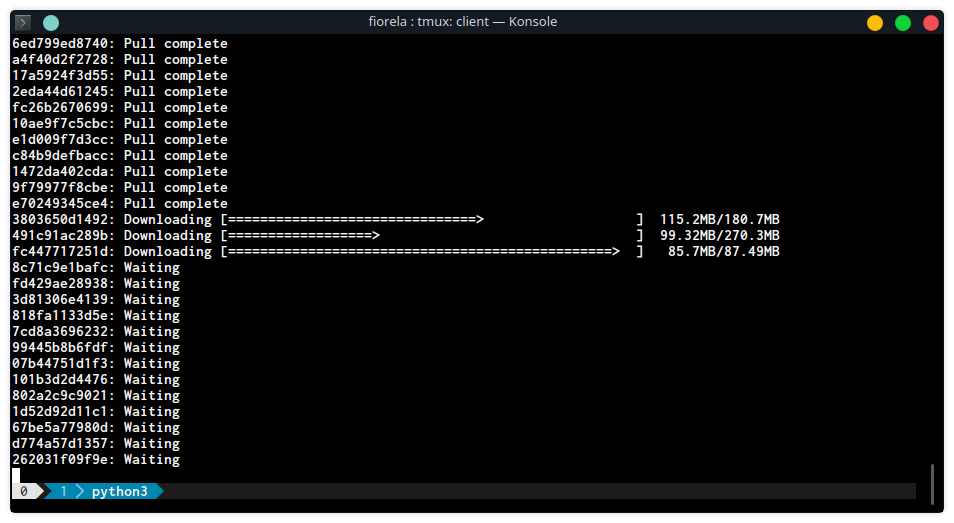
\includegraphics[scale=0.65]{./Pictures/Devilbox/015_compose_dowloads.png}
\end{figure}

Luego de que termine veremos en la terminal cómo levanta los servicios.

\begin{figure}[h!]
  \centering
  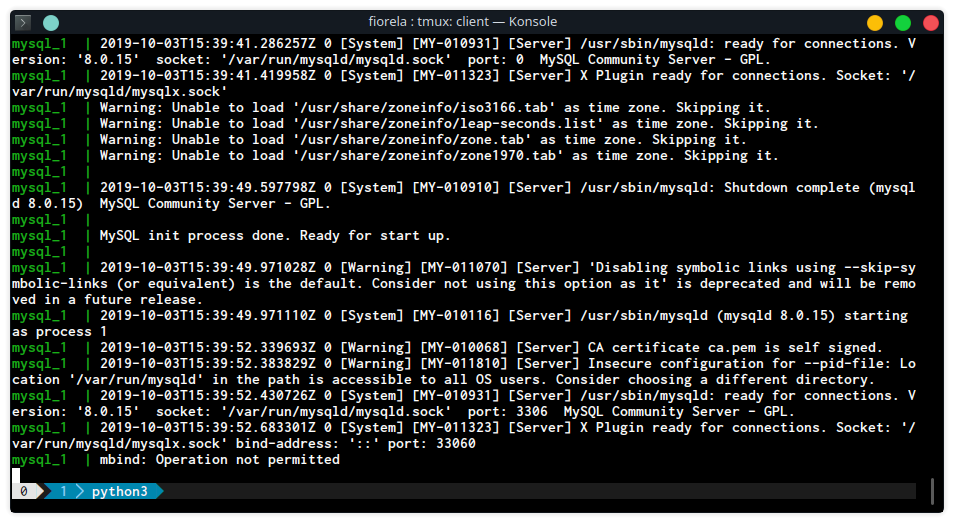
\includegraphics[scale=0.65]{./Pictures/Devilbox/016_compose_finish.png}
\end{figure}

Si en nuestro navegador vamos a \textbf{localhost} tendremos disponible el
panel de control que nos brinda \textbf{devilbox} para gestionar nuestros
proyectos.

\begin{figure}[h!]
  \centering
  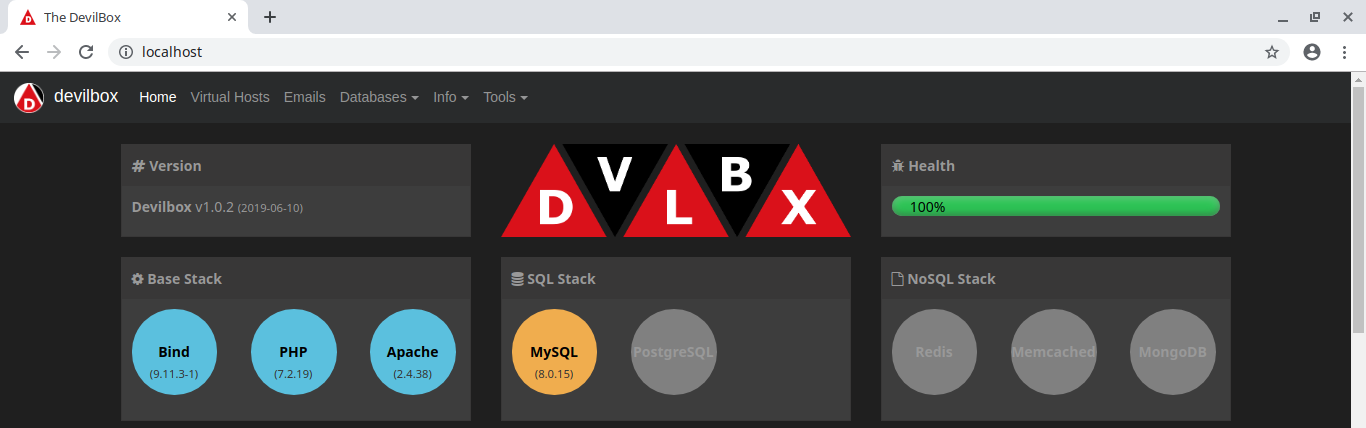
\includegraphics[scale=0.5]{./Pictures/Devilbox/017_localhost.png}
\end{figure}

Recuerda que en la terminal que hemos levantado devilbox el proceso estará
corriendo en primer plano. Para poder parar el proceso podemos presionar
\textbf{Ctrl+C}\\

\begin{figure}[h!]
  \centering
  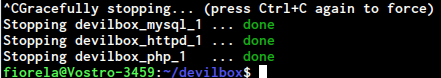
\includegraphics[scale=0.75]{./Pictures/Devilbox/018_ctrlc.png}
\end{figure}

Si queremos levantar devilbox en segundo plano y poder seguir usando nuestra
terminal para otras tareas, debemos usar el flag \textbf{-d}\\

\begin{minted}[fontsize=\footnotesize]{bash}
  docker-compose up -d httpd php mysql
\end{minted}

\begin{figure}[h!]
  \centering
  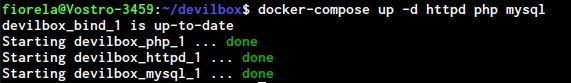
\includegraphics[scale=0.75]{./Pictures/Devilbox/019_backgroud.png}
\end{figure}

En este caso para parar el proceso deberemos ejecutar los siguientes
comandos:\\

\begin{minted}[fontsize=\footnotesize]{bash}
  docker-compose stop
  docker-composer down
\end{minted}

La principal característica de devilbox es el Auto Virtual Host. Devilbox se
encarga por si mismo de generar los dominios con el acceso que quieras darle.

\begin{figure}[h!]
  \centering
  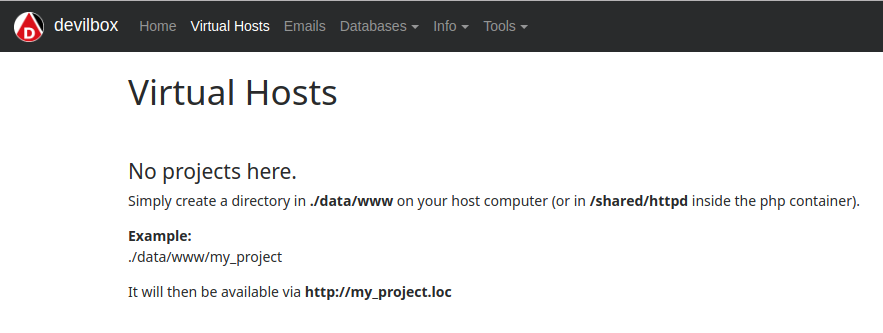
\includegraphics[scale=0.6]{./Pictures/Devilbox/020_virtual_hosts.png}
\end{figure}

Para esto deberemos crear la carpeta donde guardaremos nuestro proyecto en la
ruta \textbf{data/www}, en este caso se llamará \textbf{my\_project}.

\begin{figure}[h!]
  \centering
  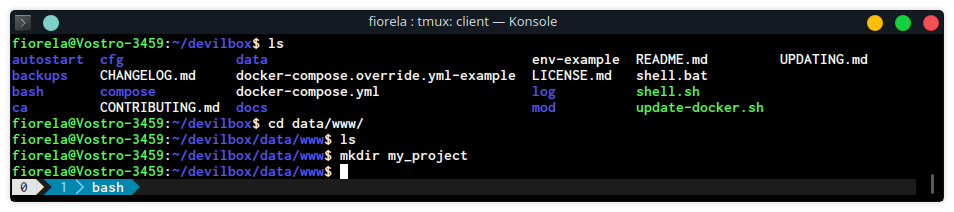
\includegraphics[scale=0.65]{./Pictures/Devilbox/021_myproject.png}
\end{figure}

Veamos como en Virtual Host ahora reconoce nuestro proyecto, pero indica un
error. Esto es porque no tenemos dentro de la carpeta creada el directorio
\textbf{htdocs}, procedemos a crearlo.\\

\newpage

\begin{figure}[h!]
  \centering
  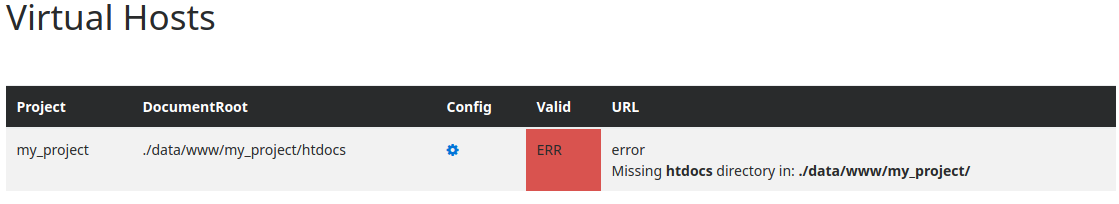
\includegraphics[scale=0.5]{./Pictures/Devilbox/022_virtual_hosts.png}
\end{figure}

\begin{minted}[fontsize=\footnotesize]{bash}
  mkdir htdocs
\end{minted}

\begin{figure}[h!]
  \centering
  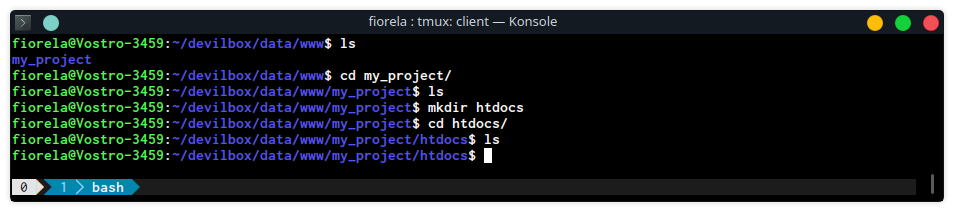
\includegraphics[scale=0.65]{./Pictures/Devilbox/023_htdocs.png}
\end{figure}

Luego de crear esta carpeta actualizamos nuestra páginas de Virtual Hosts.
Veremos esta vez un nuevo error que indica que no se ha encontrado el Host DNS.
Para solucionarlo agregamos el nombre \textbf{127.0.0.1 my\_project.loc} en
\textbf{/etc/hosts}.\\

\begin{figure}[h!]
  \centering
  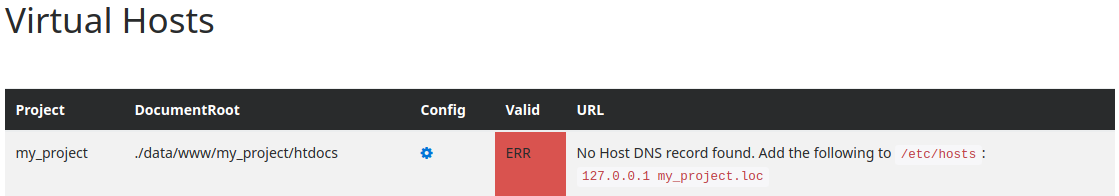
\includegraphics[scale=0.5]{./Pictures/Devilbox/024_virtual_hosts.png}
\end{figure}

\begin{figure}[h!]
  \centering
  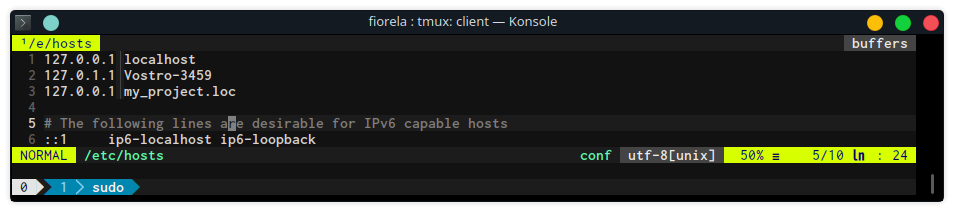
\includegraphics[scale=0.75]{./Pictures/Devilbox/025_hosts.png}
\end{figure}

Ahora podremos ingresar a este proyecto dando clic en el url.

\begin{figure}[h!]
  \centering
  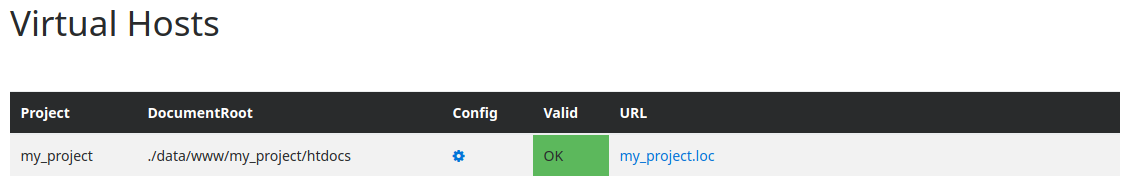
\includegraphics[scale=0.65]{./Pictures/Devilbox/026_virtual_hosts.png}
\end{figure}

Para hacer la prueba dentro de \textbf{htdocs} crearemos un fichero \textbf{index.php} con el
siguiente contenido:

\textbf{index.php}
\begin{minted}{php}
  <?php

  echo "Hola mundo!";

  ?>
\end{minted}

\begin{figure}[h!]
  \centering
  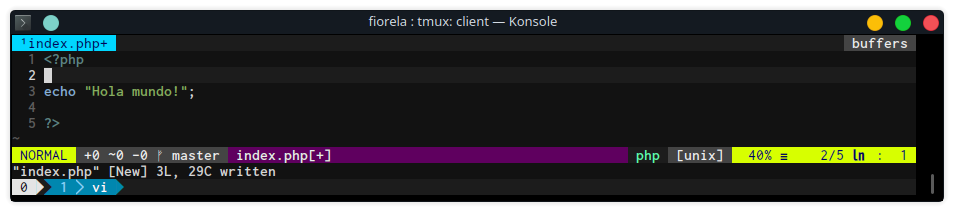
\includegraphics[scale=0.65]{./Pictures/Devilbox/027_prueba_php.png}
\end{figure}

\begin{figure}[h!]
  \centering
  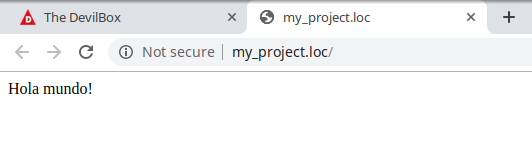
\includegraphics[scale=0.65]{./Pictures/Devilbox/028_funcional.png}
\end{figure}

Hay que resaltar que devilbox cuenta, entre otras herramientas, con phpMyAdmin
para gestionar la base de datos MySQL. Podemos acceder a esta herramienta a
través de \textbf{Tools} donde veremos otros clientes como Adminer, phpPgAdmin
para Postgress, PHPRedMin para Redis, etc.

\begin{figure}[h!]
  \centering
  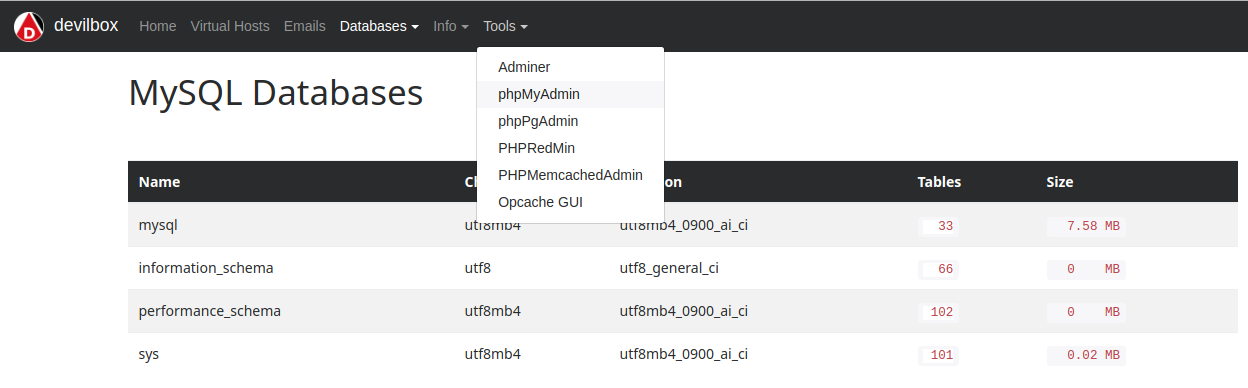
\includegraphics[scale=0.5]{./Pictures/Devilbox/030_phpMyAdmin.png}
\end{figure}

Veamos phpMyAdmin en esta ocasión:

\begin{figure}[h!]
  \centering
  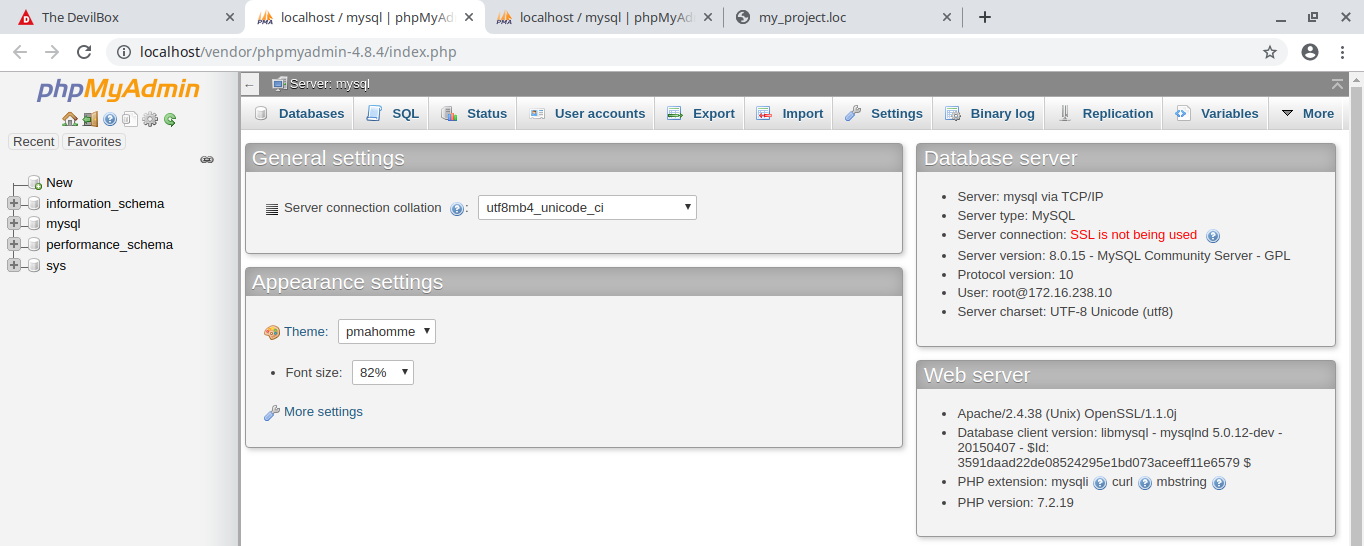
\includegraphics[scale=0.5]{./Pictures/Devilbox/031_phpMyAdmin.png}
\end{figure}

También en la pestaña \textbf{Info} podemos ver mayor información sobre el
servidor PHP o la base de datos MySQL que estamos usando.

\begin{figure}[h!]
  \centering
  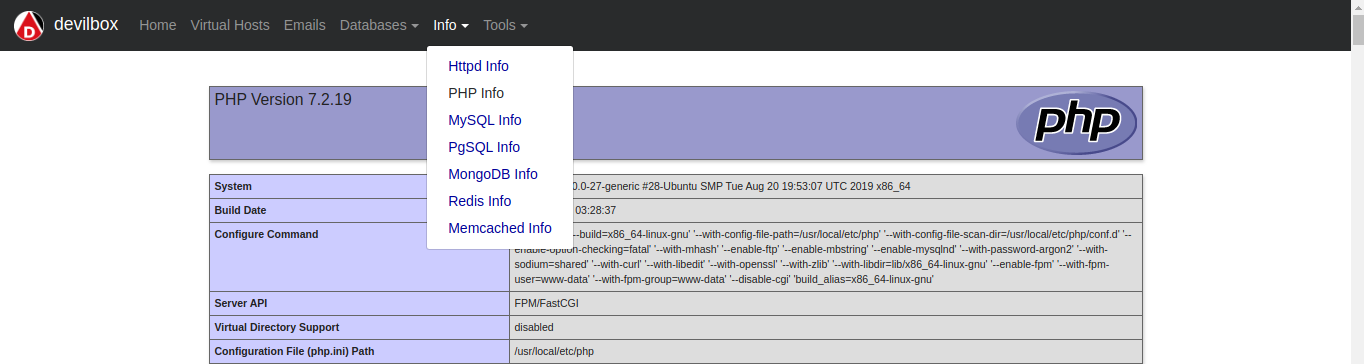
\includegraphics[scale=0.5]{./Pictures/Devilbox/032_php_info.png}
\end{figure}


%% Clase 4
\section{Revisando el template que usaremos}%
En este curso tenemos preparado un template en HTML que es muy sencillo. Visita
el siguiente enlace:\\

\textbf{index.html}
\begin{minted}[fontsize=\footnotesize]{html}
    <!doctype html>
    <html lang="en">

    <head>
      <!-- Required meta tags -->
      <meta charset="utf-8">
      <meta name="viewport" content="width=device-width, initial-scale=1,
      shrink-to-fit=no">

      <!-- Bootstrap CSS -->
      <link rel="stylesheet"
            href="https://stackpath.bootstrapcdn.com/bootstrap/4.1.2/css/bootstrap.min.css"
            integrity="sha384-Smlep5jCw/wG7hdkwQ/Z5nLIefveQRIY9nfy6xoR1uRYBtpZgI6339F5dgvm/e9B"
        crossorigin="anonymous">
      <link rel="stylesheet" href="style.css">

      <title>Resume</title>
    </head>

    <body>
      <div class="container">
        <div id="resume-header" class="row">
          <div class="col-3">
            <img id="profile-picture"
                src="https://ui-avatars.com/api/?name=John+Doe&size=255" alt="">
          </div>
          <div class="col">
            <h1>Hector Benitez</h1>
            <h2>PHP Developer</h2>
            <ul>
              <li>Mail: hector@mail.com</li>
              <li>Phone: 1234567890</li>
              <li>LinkedIn: https://linkedin.com</li>
              <li>Twitter: @hectorbenitez</li>
            </ul>
          </div>
        </div>
        <div class="row">
          <div class="col">
            <h2 class="border-bottom-gray" >Carrer Summary</h2>
            <p>
              Lorem ipsum dolor sit amet, consectetur adipiscing elit, sed do
              eiusmod tempor incididunt ut labore et dolore magna aliqua. Ut enim
              ad minim veniam, quis nostrud exercitation ullamco laboris nisi ut
              aliquip ex ea commodo consequat. Duis aute irure dolor in
              reprehenderit in voluptate velit esse cillum dolore eu fugiat nulla
              pariatur. Excepteur sint occaecat cupidatat non proident, sunt in
              culpa qui officia deserunt mollit anim id est laborum.

              Lorem ipsum dolor sit amet, consectetur adipiscing elit, sed do
              eiusmod tempor incididunt ut labore et dolore magna aliqua. Ut enim
              ad minim veniam, quis nostrud exercitation ullamco laboris nisi ut
              aliquip ex ea commodo consequat. Duis aute irure dolor in
              reprehenderit in voluptate velit esse cillum dolore eu fugiat nulla
              pariatur. Excepteur sint occaecat cupidatat non proident, sunt in
              culpa qui officia deserunt mollit anim id est laborum.
            </p>
          </div>
        </div>
        <div class="row">
          <div class="col">
            <div>
              <h3 class="border-bottom-gray" >Work Experience</h3>
              <ul>
                <li class="work-position">
                  <h5>PHP Developer</h5>
                  <p>Lorem ipsum dolor sit amet consectetur adipisicing elit. Nisi
                  sapiente sed pariatur sint exercitationem eos expedita eveniet
                  veniam ullam, quia neque facilis dicta voluptatibus. Eveniet
                  doloremque ipsum itaque obcaecati nihil.</p>
                  <strong>Achievements:</strong>
                  <ul>
                    <li>Lorem ipsum dolor sit amet, 80% consectetuer adipiscing elit.</li>
                    <li>Lorem ipsum dolor sit amet, 80% consectetuer adipiscing elit.</li>
                    <li>Lorem ipsum dolor sit amet, 80% consectetuer adipiscing elit.</li>
                  </ul>
                </li>
                <li class="work-position">
                    <h5>PHP Developer</h5>
                    <p>Lorem ipsum dolor sit amet consectetur adipisicing elit.
                    Nisi sapiente sed pariatur sint exercitationem eos expedita
                    eveniet veniam ullam, quia neque facilis dicta voluptatibus.
                    Eveniet doloremque ipsum itaque obcaecati nihil.</p>
                    <strong>Achievements:</strong>
                    <ul>
                      <li>Lorem ipsum dolor sit amet, 80% consectetuer adipiscing elit.</li>
                      <li>Lorem ipsum dolor sit amet, 80% consectetuer adipiscing elit.</li>
                      <li>Lorem ipsum dolor sit amet, 80% consectetuer adipiscing elit.</li>
                    </ul>
                  </li>
                  <li class="work-position">
                      <h5>PHP Developer</h5>
                      <p>Lorem ipsum dolor sit amet consectetur adipisicing elit.
                      Nisi sapiente sed pariatur sint exercitationem eos expedita
                      eveniet veniam ullam, quia neque facilis dicta voluptatibus.
                      Eveniet doloremque ipsum itaque obcaecati nihil.</p>
                      <strong>Achievements:</strong>
                      <ul>
                        <li>Lorem ipsum dolor sit amet, 80% consectetuer adipiscing elit.</li>
                        <li>Lorem ipsum dolor sit amet, 80% consectetuer adipiscing elit.</li>
                        <li>Lorem ipsum dolor sit amet, 80% consectetuer adipiscing elit.</li>
                      </ul>
                    </li>
              </ul>
            </div>
            <div>
                <h3 class="border-bottom-gray">Projects</h3>
                <div class="project">
                    <h5>Project X</h5>
                    <div class="row">
                        <div class="col-3">
                            <img id="profile-picture" src="https://ui-avatars.com/api/?name=John+Doe&size=255" alt="">
                          </div>
                          <div class="col">
                            <p>Lorem ipsum dolor sit amet consectetur adipisicing
                            elit. Eius earum corporis at accusamus quisquam hic
                            quos vel? Tenetur, ullam veniam consequatur esse quod
                            cum, quam cupiditate assumenda natus maiores
                            aperiam.</p>
                            <strong>Technologies used:</strong>
                            <span class="badge badge-secondary">PHP</span>
                            <span class="badge badge-secondary">HTML</span>
                            <span class="badge badge-secondary">CSS</span>
                          </div>
                    </div>
                </div>
                <div class="project">
                    <h5>Project X</h5>
                    <div class="row">
                        <div class="col-3">
                            <img id="profile-picture" src="https://ui-avatars.com/api/?name=John+Doe&size=255" alt="">
                          </div>
                          <div class="col">
                            <p>Lorem ipsum dolor sit amet consectetur adipisicing
                            elit. Eius earum corporis at accusamus quisquam hic
                            quos vel? Tenetur, ullam veniam consequatur esse quod
                            cum, quam cupiditate assumenda natus maiores
                            aperiam.</p>
                            <strong>Technologies used:</strong>
                            <span class="badge badge-secondary">PHP</span>
                            <span class="badge badge-secondary">HTML</span>
                            <span class="badge badge-secondary">CSS</span>
                          </div>
                    </div>
                </div>
              </div>
          </div>
          <div class="col-3">
            <h3 class="border-bottom-gray" >Skills & Tools</h3>
            <h4>Backend</h4>
            <ul>
              <li>PHP</li>
            </ul>
            <h4>Frontend</h4>
            <ul>
                <li>HTML</li>
                <li>CSS</li>
            </ul>
            <h4>Frameworks</h4>
            <ul>
              <li>Laravel</li>
              <li>Bootstrap</li>
            </ul>
            <h3 class="border-bottom-gray" >Languages</h3>
            <ul>
              <li>Spanish</li>
              <li>English</li>
            </ul>
          </div>
        </div>
        <div id="resume-footer" class="row">
          <div class="col">
              Designed by @hectorbenitez
          </div>
        </div>
      </div>

      <!-- Optional JavaScript -->
      <!-- jQuery first, then Popper.js, then Bootstrap JS -->
      <script src="https://code.jquery.com/jquery-3.3.1.slim.min.js"
              integrity="sha384-q8i/X+965DzO0rT7abK41JStQIAqVgRVzpbzo5smXKp4YfRvH+8abtTE1Pi6jizo"
        crossorigin="anonymous"></script>
      <script
        src="https://cdnjs.cloudflare.com/ajax/libs/popper.js/1.14.3/umd/popper.min.js"
        integrity="sha384-ZMP7rVo3mIykV+2+9J3UJ46jBk0WLaUAdn689aCwoqbBJiSnjAK/l8WvCWPIPm49"
        crossorigin="anonymous"></script>
      <script
        src="https://stackpath.bootstrapcdn.com/bootstrap/4.1.2/js/bootstrap.min.js"
        integrity="sha384-o+RDsa0aLu++PJvFqy8fFScvbHFLtbvScb8AjopnFD+iEQ7wo/CG0xlczd+2O/em"
        crossorigin="anonymous"></script>
    </body>

    </html>
\end{minted}

\textbf{style.css}
\begin{minted}{css}
  #resume-header {
      margin-top: 20px;
      margin-bottom: 20px;
  }

  #profile-picture {
      width: 100%;
  }

  #resume-footer {
      padding: 20px;
      text-align: center;
  }

  .border-bottom-gray {
      padding-bottom: 10px;
      border-bottom: solid 1px darkgray;
  }

  .work-position {
      margin-bottom: 40px;
  }

  .project {
      margin-bottom: 40px;
  }
\end{minted}

\begin{itemize}
  \item Descarga los archivos en tu computadora (encuentra el repositorio en
    pestaña de archivos).
  \item Ingresa a www dentro de devilbox. Debe aparecer:
    \$HOME/devilbox/data/www/
  \item Crea y nombra una nueva carpeta. (ejemplo: my\_project o remake)
  \item Copia los archivos del template (index.html y style.css).
\end{itemize}

\newpage

\begin{figure}[h!]
  \centering
  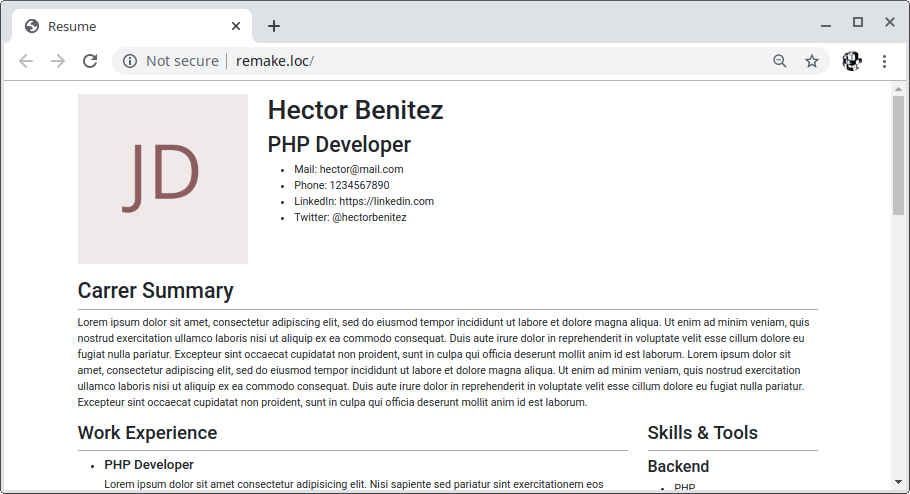
\includegraphics[scale=0.5]{./Pictures/008_template.png}
\end{figure}

%% Clase 5
\section{Sintaxis de PHP}%
Hagamos el ejemplo más sencillo para trabajar con PHP. Siempre que usemos PHP
usaremos lo siguiente: $<$?php ?$>$ todo lo que pongamos dentro de esto será lo
que el servidor va a interpretar como código php, lo que esté fuera lo
ignorará.\\

\textbf{hello.php}\\
\begin{minted}{php}
  <?php
  echo 'Hola PHP';
  ?>
\end{minted}

\begin{figure}[h!]
  \centering
  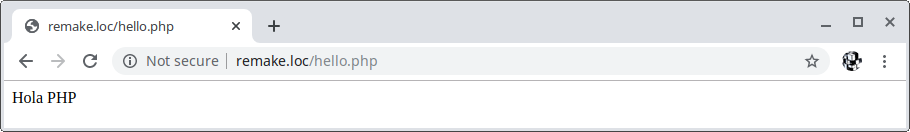
\includegraphics[scale=0.75]{./Pictures/009_hellophp.png}
\end{figure}

Para acceder a él lo haremos /hello.php porque el servidor abre por defecto el
archivo index y nuestro nuevo archivo se llama hello.php.\\

\textbf{index.html  ln:27-36}
\begin{minted}{html+php}
        <div class="col">
          <h1><?php echo 'Hector Benitez'; ?></h1>
          <h2>PHP Developer</h2>
          <ul>
            <li>Mail: hector@mail.com</li>
            <li>Phone: 1234567890</li>
            <li>LinkedIn: https://linkedin.com</li>
            <li>Twitter: @hectorbenitez</li>
          </ul>
        </div>
\end{minted}

\newpage

\begin{figure}[h!]
  \centering
  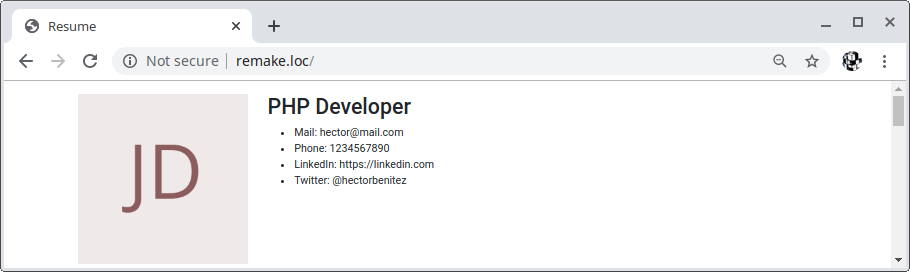
\includegraphics[scale=0.5]{./Pictures/010_indexhtml.png}
\end{figure}

Si queremos escribir código php en nuestra vista HTML tendremos que cambiarle
la extensión al archivo por .php porque nuestro servidor esta configurado a
solo interpretar archivos PHP. Solo las partes dentro de <?php ?> van a ser
interpretadas y su código fuente no será visible desde el navegador.\\

Todas las sentencias de código se separarán con un ; (punto y coma).\\

\begin{figure}[h!]
  \centering
  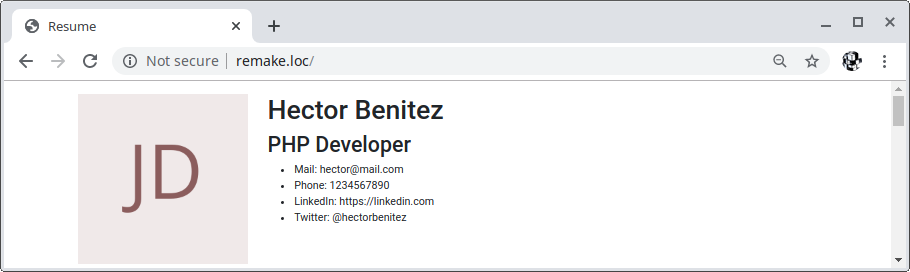
\includegraphics[scale=0.5]{./Pictures/011_indexphp.png}
\end{figure}


%% Clase 6
\section{Variables tipos de datos y cadenas}%
Es importante conocer que el código en cada bloque de código php se comparte en
todo el documento, así si declaras una variable en un bloque podrás usarlo en
otro bloque al final.\\

Una variable puede ser una pequeña cajita en la que puedes almacenar un valor y
este lo pueden usar para realizar alguna operación.\\

Para declararla usaremos el símbolo de \$ y en seguida el nombre, este puede ser
un \_ o una letra.\\

\textbf{index.php  ln:1-7 y 32-41}
\begin{minted}{html+php}
  <?php
  $var1 = 1;
  $name = 'Hector';
  ?>

  <!doctype html>
  <html lang="en">
  ...
        <div class="col">
          <h1><?php echo $name; ?></h1>
          <h2>PHP Developer</h2>
          <ul>
            <li>Mail: hector@mail.com</li>
            <li>Phone: 1234567890</li>
            <li>LinkedIn: https://linkedin.com</li>
            <li>Twitter: @hectorbenitez</li>
          </ul>
        </div>
  ...
\end{minted}

\begin{figure}[h!]
  \centering
  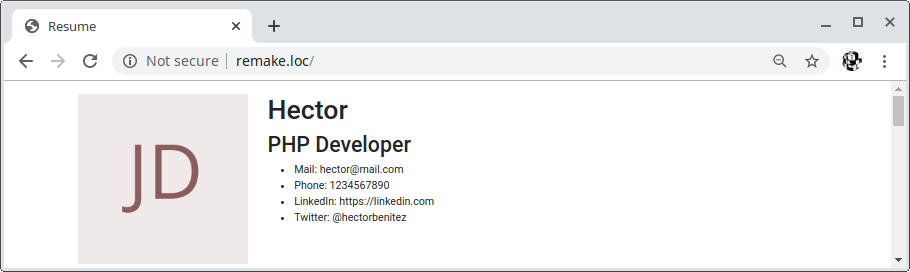
\includegraphics[scale=0.5]{./Pictures/012_variables.png}
\end{figure}

PHP no es estáticamente tipado, es decir que no tenemos que decirle qué tipo de
dato es esa variable. Además, es débilmente tipado porque podemos fácilmente
cambiar el tipo de dato, es decir PHP ejecuta una conversión de datos interna.\\

\textbf{index.php ln 1-5}
\begin{minted}{html+php}
  <?php
  $var1 = 1;
  $name = 'Hector';
  $name = 123;
  ?>
\end{minted}

\begin{figure}[h!]
  \centering
  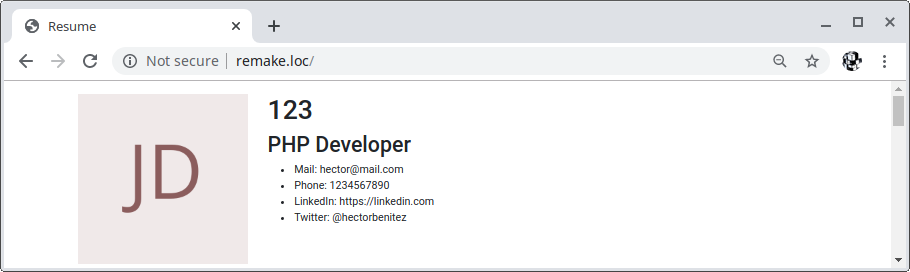
\includegraphics[scale=0.5]{./Pictures/013_variables.png}
\end{figure}

Al momento de trabajar con PHP una cosa muy importante es hacer debugging a
nuestras variables, para ello utilizamos la función var\_dump(); pasándole por
parámetro la variable a revisar.\\

\textbf{index.php ln 1-4}
\begin{minted}{html+php}
  <?php
  $name = 'Hector';
  var_dump($name);
  ?>
\end{minted}

\begin{figure}[h!]
  \centering
  \includegraphics[scale=0.5]{./Pictures/014_vardump.png}
\end{figure}

\newpage

A diferencia de otros lenguajes en PHP para concatenar strings se usa el
punto:\\

\textbf{index.php ln 1-4}
\begin{minted}{html+php}
  <?php
  $lastname = 'Benitez';
  $name = 'Hector' . $lastname;
  ?>
\end{minted}

\begin{figure}[h!]
  \centering
  \includegraphics[scale=0.5]{./Pictures/015_concatenar_punto.png}
\end{figure}

En PHP tenemos dos tipos de cadenas, las que son con comillas simples y las de
comillas dobles. La diferencia entre estas dos cadenas es que la de comillas
simples recibe de forma literal lo que le escribas mientras que la de comillas
dobles intenta interpretar cualquier variable dentro de ella.\\


\textbf{index.php ln 1-4}
\begin{minted}{php}
  <?php
  $lastname = 'Benitez';
  $nombre = "Hector $lastname";
  ?>
\end{minted}

\begin{figure}[h!]
  \centering
  \includegraphics[scale=0.5]{./Pictures/016_doble_comilla.png}
\end{figure}

\textbf{index.php ln 1-4}
\begin{minted}{php}
  <?php
  $lastname = 'Benitez';
  $nombre = 'Hector $lastname';
  ?>
\end{minted}

\begin{figure}[h!]
  \centering
  \includegraphics[scale=0.5]{./Pictures/017_comilla_simple.png}
\end{figure}


%% Clase 7

\section{Tipos de Datos en PHP}%
PHP cuenta con muchos tipos de datos, sin embargo, en este momento nos vamos a
enfocar en los más importantes y utilizados que son boolean, integer, float,
string, array y NULL.\\

\subsection*{Tipos escalares:}%
\textbf{boolean}:\\
Representa solamente un valor verdadero o falso.
\href{http://php.net/manual/es/language.types.boolean.php}{Enlace}.\\
Valores válidos: true (verdadero), false (falso).

\begin{minted}{php}
  <?php
    $a = true;
    $b = false;
  ?>
\end{minted}

\textbf{Integer}:\\
Representa un número entero positivo, negativo o 0.
\href{http://php.net/manual/es/language.types.integer.php}{Enlace}.\\

\begin{minted}{php}
  <?php
    $a = -123;
    $b = 0;
    $c = 7763;
  ?>
\end{minted}

\textbf{float o double}:\\
Representa un número de punto flotante, existen problemas de precisión con los
números flotantes debido a la naturaleza binaria de las computadoras.
\href{http://php.net/manual/es/language.types.float.php}{Enlace}.\\

\begin{minted}{php}
  <?php
    $a = 12.24; 
    $b = 1.5e3; 
    $c = 7E-10;
  ?> 
\end{minted}

\textbf{string:}\\
- Representa una cadena de caracteres.\\
- Existen 4 formas de representar una cadena. Las 2 principales son usando
comillas simples o comillas dobles.\\
\begin{itemize}
  \item Usando comillas simples donde el texto será exactamente como se escribe.
  \item Usando comillas dobles permite usar caracteres de escape y además
    expanden los nombres de las variables, es decir sustituye el valor de las
    variables dentro de las cadenas.
\end{itemize}
– Hay 2 formas adicionales llamadas Heredoc y Nowdoc que sirven para crear
cadenas de múltiples líneas.\\

Si quieres conocer más de este tipo de dato da
\href{http://php.net/manual/es/language.types.string.php#language.types.string.details}{click
aquí}.\\

\begin{minted}{php}
  <?php
    $a = ”Hola”; 
    $b = ‘Mundo’; 
  ?>
\end{minted}

\subsection*{Tipos compuestos:}%
\textbf{array}:\\
Representa una colección de valores, aunque por defecto PHP usara índices
numéricos, la realidad es que la estructura se representa como un mapa que
colecciona pares llave-valor. La sintaxis para definir un arreglo será a partir
de corchetes cuadrados, aunque en versiones anteriores de PHP era necesario
usar la función array(). Las llaves pueden ser enteros o cadenas y los valores
pueden ser de cualquier tipo de PHP, incluso de tipo array.
\href{http://php.net/manual/es/language.types.array.php}{Enlace}.\\

\begin{minted}{php}
  <?php
  $array = array(
    "curso1" => "php",
    "curso2" => "js",
  );


  // a partir de PHP 5.4
  $array = [
    "curso1" => "php",
    "curso2" => "js",
  ];

  // índices numéricos
  $array = [
    "php",
    "js",
  ];
  ?>
\end{minted}

\textbf{object}:\\
Representa una instancia de una clase. Este tema lo veremos más a fondo en la
clase de Programación Orientada a Objetos.\\

\begin{minted}{php}
  <?php
  class Car
  {
        function move()
        {
                  echo "Going forward..."; 
        }
  }

  $myCar = new Car();
  $myCar->move();
  ?>
\end{minted}

\newpage

\textbf{callable}:
Es un tipo de dato especial que representa a algo que puede ser “llamado”, por
ejemplo una función o un método.\\

\begin{minted}{php}
  <?php
  // Variable que guarda un callable
  $firstOfArray = function(array $array) {
        if (count($array) == 0) { return null;  }
            return $array[0];
  };

  // Este es nuestro arreglo
  $values = [3, 2, 1];

  // Usamos nuestro callable y se imprime el valor 3
  echo $firstOfArray($values);
  ?>
\end{minted}

\textbf{iterable}:\\
A partir de PHP 7.1 iterable es un pseudo tipo de datos que puede ser
recorrido.\\

\begin{minted}{php}
  <?php

  function foo(iterable $iterable) {
    foreach ($iterable as $valor) {
              // ...
    }
  }

  ?>
\end{minted}

\subsection*{Tipos especiales:}%
\textbf{resource}:\\
Es un tipo de dato especial que representa un recurso externo, por ejemplo un
archivo externo a tu aplicación.\\

\begin{minted}{php}
  <?php
    $res = fopen("c:\\dir\\file.txt", "r");
  ?>
\end{minted}

\textbf{NULL}:\\
Es un valor especial que se usa para representar una variable sin valor.
\href{http://php.net/manual/es/language.types.null.php}{Enlace}.\\

\begin{minted}{php}
  <?php
    $a = null;
  ?>
\end{minted}

\newpage

%% Clase 8
\section{Arreglos}%
Como vimos en la clase anterior almacenamos datos en una variable, ahora
trataremos de almacenar más datos en una misma variable.\\

Estas variables que almacenan más de un dato se conocen como arreglos y su
sintaxis se va a indicar con $[$  $]$ (corchetes).\\

\textbf{index.php ln 1-10 59-60 69-70 79-80}
\begin{minted}{php}
  <?php
  $name = 'Hector Benitez';
  $jobs = [
    'PHP Developer',
    'Python Dev',
    'Devops'
  ];

  var_dump($jobs);
  ?>
  ...
      <li class="work-position">
        <h5><?php echo $jobs[0]; ?></h5>
  ...
      <li class="work-position">
          <h5> <?php echo $jobs[1]; ?></h5>
  ...
      <li class="work-position">
          <h5><?php echo $jobs[2]; ?></h5>
  ...
\end{minted}

\begin{figure}[h!]
  \centering
  \includegraphics[scale=0.5]{./Pictures/018_array.png}
\end{figure}

\begin{figure}[h!]
  \centering
  \includegraphics[scale=0.5]{./Pictures/019_array.png}
\end{figure}

PHP utiliza índices para localizar a los elementos dentro de la variable.\\

La estructura de arreglos en PHP es conocida como mapa, lo que quiere decir que
tiene una composición de llave valor. Además, un arreglo puede contener más
arreglos y cada uno de ellos seguirá la misma estructura.\\

\newpage

\textbf{index.php ln 1-15 65-66 75 85}
\begin{minted}{php}
  <?php
  $name = 'Hector Benitez';
  $jobs = [
    [
      'title' => 'PHP Developer',
      'description' => 'This is an awesome job!!!'
    ],
    [
      'title' => 'Python Dev',
    ],
    [
      'title' => 'Devops'
    ]
  ];
  ?>
  ...
        <h5><?php echo $jobs[0]['title']; ?></h5>
        <p><?php echo $jobs[0]['description']; ?></p>
  ...
        <h5> <?php echo $jobs[1]['title']; ?></h5>
  ...
        <h5><?php echo $jobs[2]['title']; ?></h5>
  ...
\end{minted}

\begin{figure}[h!]
  \centering
  \includegraphics[scale=0.5]{./Pictures/020_array_array.png}
\end{figure}

Algo que debes saber es que en PHP podrás almacenar diferentes tipos de datos
en un mismo arreglo.\\

\newpage

%% Clase 9
\section{Ejercicios Arreglos}%
\subsection*{Ejercicio 1.}%
Escribe el código necesario para generar la cadena final usando el arreglo dado\\
\begin{minted}{php}
  $arreglo = [
    ‘keyStr1’ => ‘lado’,
    0 => ‘ledo’,

    ‘keyStr2’ => ‘lido’,
    1 => ‘lodo’,
    2 => ‘ludo’
  ];
\end{minted}

Lado, ledo, lido, lodo, ludo,
decirlo al revés lo dudo.
Ludo, lodo, lido, ledo, lado,
¡Qué trabajo me ha costado!

\subsection*{Ejercicio 2.}%
Crea un arreglo que contenga como clave los nombres de 5 países y como valor
otro arreglo con 3 ciudades que pertenezcan a ese país, después utiliza un
ciclo foreach, para imprimir el nombre del país seguido de las ciudades que
definiste:\\

Ejemplo,
\textbf{México}: Monterrey Querétaro Guadalajara
\textbf{Colombia}: Bogota Cartagena Medellin

\subsection*{Ejercicio 3.}%
Escribe el código necesario para encontrar los 3 números más grandes y los 3
números más bajos de la siguiente lista:\\
\begin{minted}{php}
  $valores = [23, 54, 32, 67, 34, 78, 98, 56, 21, 34, 57, 92, 12, 5, 61];
\end{minted}

Veamos la solución:\\

\textbf{arreglos.php}
\begin{minted}{php}
  <?php
  echo "Ejercicio 1\n";
  $arreglo = [
    'keyStr1' => 'lado',
    0 => 'ledo',
    'keyStr1' => 'lido',
    1 => 'lodo',
    2 => 'ludo'
  ];

  foreach ($arreglo as $key => $value) {
    if ($key === 'keyStr1') {
      echo ucfirst($value) . ', ';
    } else {
      echo $value . ', ';
    }
  }

  $arrayReverse = array_reverse($arreglo);
  echo "\n";
  echo "decirlo al revés lo dudo.";
  echo "\n";

  foreach ($arrayReverse as $key => $value) {
    if ($key === 0) {
      echo ucfirst($value) . ', ';
    } else {
      echo $value . ', ';
    }
  }
  echo "\n";
  echo "¡Qué trabajo me ha costado!\n\n";

  echo "Ejercicio 2\n";
  $countries = [
    'Peru' => ['Lima', 'Cusco', 'Arequipa'],
    'Chile' => ['Santiago', 'Antofagasta', 'Arica'],
    'Bolivia' => ['Sucre', 'Cochabamba', 'La paz'],
    'Colombia' => ['Bogota', 'Cartagena', 'Medellin'],
    'México' => ['Monterrey', 'Querétaro', 'Guadalajara']
  ];

  foreach ($countries as $pais => $ciudad) {
    echo "$pais: ";
    foreach ($ciudad as $value) {
      echo "$value ";
    }
    echo "\n";
  }

  echo "\nEjercicio 3\n";
  $valores = [23, 54, 32, 67, 34, 78, 98, 56, 21, 34, 57, 92, 12, 5, 61];
  rsort($valores);
  for ($i = 0; $i < 3; $i++) {
    echo "$valores[$i], ";
  }
  echo "\n";
  sort($valores);
  for ($i = 0; $i < 3; $i++) {
    echo "$valores[$i], ";
  }
  ?>
\end{minted}

\newpage

\begin{figure}[h!]
  \centering
  \includegraphics[scale=0.75]{./Pictures/021_ejercicios.png}
\end{figure}


%% Clase 10
\section{Condicionales y Ciclos}%
Las condiciones nos permiten tomar decisiones en el código, si se cumple la
condición entonces se ejecutarán ciertas instrucciones sino se cumple se
ejecutarán otras. Estas se denotan por la instrucción if else.\\

\begin{minted}{php}
  <?php
  $var1 = 5;
  if ($var1 > 2) {
    echo "es mayor que 2\n";
  } else {
    echo "no es mayor que 2\n";
  }
  ?>
\end{minted}

\begin{figure}[h!]
  \centering
  \includegraphics[scale=0.75]{./Pictures/031_condicional.png}
\end{figure}

Los ciclos funcionan de la mano con las condiciones, en este caso si se cumple
la instrucción se estará ejecutando repetidas veces una instrucción dada.\\

Hemos agregado los jobs de forma manual accediendo al arreglo a través de sus
índices, hacer esto podría traer errores y no podríamos controlarlo si
tuviéramos muchos jobs. Ahora veamos una mejor forma de hacerlo con ciclos.\\

\begin{itemize}
  \item El primero que tenemos es do while que va a involucrar la
    inicialización de variables y condiciones.
  \item El segundo que veremos es for que es una forma más simplificada de usar
    todos los elementos que componen los ciclos.
\end{itemize}

\textbf{index.php ln 1-17 66-81 82-101(eliminar)}
\begin{minted}{php}
  <?php
  $name = 'Hector Benitez';
  $jobs = [
    [
      'title' => 'PHP Developer',
      'description' => 'This is an awesome job!!!'
    ],
    [
      'title' => 'Python Dev',
      'description' => 'This is an awesome job!!!'
    ],
    [
      'title' => 'Devops',
      'description' => 'This is an awesome job!!!'
    ]
  ];
  ?>
  ...
          <?php
          $idx = 0;
          do {
            echo '<li class="work-position">';
            echo '<h5>' . $jobs[$idx]['title'] . '</h5>';
            echo '<p>' . $jobs[$idx]['description'] . '</p>';
            echo '<strong>Achievements:</strong>';
            echo '<ul>';
            echo '<li>Lorem ipsum dolor sit amet, 80% consectetuer adipiscing elit.</li>';
            echo '<li>Lorem ipsum dolor sit amet, 80% consectetuer adipiscing elit.</li>';
            echo '<li>Lorem ipsum dolor sit amet, 80% consectetuer adipiscing elit.</li>';
            echo '</ul>';
            echo '</li>';
            $idx = $idx + 1;
          } while($idx < 3);
          ?>
  ...
\end{minted}

\textbf{index.php ln 68-77}
\begin{minted}{php}
  <?php
  ...
        for ($idx = 0; $idx < count($jobs); $idx++) {
          echo '<li class="work-position">';
          echo '<h5>' . $jobs[$idx]['title'] . '</h5>';
          echo '<p>' . $jobs[$idx]['description'] . '</p>';
          echo '<strong>Achievements:</strong>';
          echo '<ul>';
          echo '<li>Lorem ipsum dolor sit amet, 80% consectetuer adipiscing elit.</li>';
          echo '<li>Lorem ipsum dolor sit amet, 80% consectetuer adipiscing elit.</li>';
          echo '<li>Lorem ipsum dolor sit amet, 80% consectetuer adipiscing elit.</li>';
          echo '</ul>';
          echo '</li>';
        }
  ...
  ?>
\end{minted}

\newpage

\begin{figure}[h!]
  \centering
  \includegraphics[scale=0.5]{./Pictures/032_bucles.png}
\end{figure}


%% Clase 11
\section{While vs. Do While}%
\subsection*{Ciclos}%
Como mencionamos en nuestra clase anterior, los ciclos o bucles son de total
importancia cuando desarrollamos software pues nos permiten repetir un bloque
de acciones y en consecuencia re-utilizar mejor nuestro código, en este momento
ya hablamos de cómo funciona el ciclo for y el ciclo do-while.\\

Ahora vamos a revisar un par de ciclos adicionales en PHP los cuales también es
importante conocer. Toma en cuenta que la mayoría de las cosas se pueden hacer
de diferentes maneras por lo tanto es importante que elijas bien cual es el
ciclo que mejor se adapta a tu problema.\\

\subsection*{while vs. do… while}%
En la clase anterior hablamos del ciclo do while, aquí lo compararemos con otro
ciclo llamado while, recapitulemos el funcionamiento de do… while:\\

Cuando creamos un ciclo do… while, le decimos a PHP que ejecute cierto bloque
de código siempre y cuando la condición que tengas dentro se siga evaluando
como verdadera.\\

Esta es la sintaxis de un ciclo do… while\\

\begin{minted}{php}
  <?php
  do {
    codigo...
  } while (condicion);
  ?>
\end{minted}

El ciclo while funciona de la misma manera, pero la diferencia principal es que
la evaluación se llevará a cabo al iniciar el ciclo:\\

\begin{minted}{php}
  <?php
  while (condicion) {
    codigo...
  }
  ?>
\end{minted}

La principal diferencia es que el ciclo do while garantiza que el código
interno se ejecutará al menos 1 vez, mientras que en el ciclo while si la
condición es falsa desde un inicio, es posible que el ciclo nunca se ejecute

\href{http://php.net/manual/es/control-structures.while.php}{Manual while}
\href{http://php.net/manual/es/control-structures.do.while.php}{Manual Do While}

\subsection*{Foreach}%
El ciclo foreach nos brinda una solución simple para iterar sobre los valores
de un arreglo, la sintaxis es la siguiente:\\

\begin{minted}{php}
  <?php
  foreach ($array as $valor) {
    sentencias que pueden usar $valor
  }
  ?>
\end{minted}

En esta sintaxis nos encontramos con 4 partes:

\begin{itemize}
  \item La palabra reservada foreach simplemente indica el inicio de nuestro bloque
  \item Dentro de paréntesis se escribe el nombre del arreglo que vamos a estar
    iterando, este arreglo debe estar definido previamente, en este ejemplo es
    \$arreglo
  \item La palabra “as” seguido de un nombre de variable que usaremos para
    acceder al elemento del arreglo que estamos accediendo, esta variable no
    debe existir previamente y solo la podrán usar dentro de este bloque. En el
    ejemplo es \$valor.
  \item Entre llaves todas las acciones que queremos repetir, en el momento en
    que se ejecute el ciclo la variable que definimos para iterar (en el
    ejemplo \$valor) ya existe y podrá ser usada en esta sección, piensa que el
    valor de esta variable estará cambiando en cada iteración.
\end{itemize}

Suponiendo que en el ejemplo anterior \$array = $[$‘uno’, ‘dos’, ‘tres’$]$, el ciclo
se repetirá 3 veces y en cada iteración la variable \$valor contendrá el
elemento del arreglo correspondiente, es decir, en la primera iteración \$valor
será igual a ‘uno’, en la segunda \$valor será igual a ‘dos’ y en la tercera
\$valor será igual a ‘tres’.

Existe una sintaxis alternativa que nos permite no solo conocer el valor,
también nos permitirá conocer la llave, de este modo tendremos acceso tanto a
la llave como al valor del elemento del arreglo:\\

\href{http://php.net/manual/es/control-structures.foreach.php}{Manual Foreach}


%% Clase 12
\section{Operadores, Condicionales, Continue y Break}%
En PHP existen cuatro tipos principales de operadores:

\begin{itemize}
  \item Aritméticos.
  \item Asignación.
  \item Condicionales.
  \item Incremento.
\end{itemize}

Aprovechemos para practicar y veamos más sobre condiciones, en PHP tenemos el
operador de comparación (==) y diferente de (!=).\\

Tenemos la sentencia continue la cuál al ejecutarse hará que se itere a la
siguiente línea del arreglo. Y la sentencia break que hará que el ciclo se
termine.\\

Usando esto en nuestro proyecto, por ejemplo haremos que se muestren las
experiencias laborales que hayamos tenido dentro de los 12 meses y que
consideremos \textbf{visibles}. Veamos el código.\\

\textbf{index.php ln 1-36 85-108}
\begin{minted}{php}
  <?php
  $name = 'Hector Benitez';
  $limitMonths = 12;
  $jobs = [
    [
      'title' => 'PHP Developer',
      'description' => 'This is an awesome job!!!',
      'visible' => true,
      'months' => 6
    ],
    [
      'title' => 'Python Dev',
      'description' => 'This is an awesome job!!!',
      'visible' => false,
      'months' => 4
    ],
    [
      'title' => 'Devops',
      'description' => 'This is an awesome job!!!',
      'visible' => false,
      'months' => 5
    ],
    [
      'title' => 'Node Dev',
      'description' => 'This is an awesome job!!!',
      'visible' => true,
      'months' => 2
    ],
    [
      'title' => 'Fronted Dev',
      'description' => 'This is an awesome job!!!',
      'visible' => true,
      'months' => 3
    ]
  ];
  ?>
  ...
        <?php
          $totalMonths = 0;
          for ($idx = 0; $idx < count($jobs); $idx++) {
            $totalMonths += $jobs[$idx]['months'];

            if ($totalMonths > $limitMonths) {
              break;
            }
            if($jobs[$idx]['visible'] == false) {
              continue;
            }

            echo '<li class="work-position">';
            echo '<h5>' . $jobs[$idx]['title'] . '</h5>';
            echo '<p>' . $jobs[$idx]['description'] . '</p>';
            echo '<strong>Achievements:</strong>';
            echo '<ul>';
            echo '<li>Lorem ipsum dolor sit amet, 80% consectetuer adipiscing elit.</li>';
            echo '<li>Lorem ipsum dolor sit amet, 80% consectetuer adipiscing elit.</li>';
            echo '<li>Lorem ipsum dolor sit amet, 80% consectetuer adipiscing elit.</li>';
            echo '</ul>';
            echo '</li>';
          }
        ?>
  ...
\end{minted}

\begin{figure}[h!]
  \centering
  \includegraphics[scale=0.5]{./Pictures/033_opeadores.png}
\end{figure}



%% Clase 13
\section{Operadores}%
Antes de continuar hablando de operadores es importante mencionar que existe un
concepto conocido como precedencia de operadores el cual nos permitirá saber en
qué orden se deben ejecutar los operadores que se encuentren en una sola
sentencia.\\

Por ejemplo, en la sentencia:\\

1 + 2 * 3\\

Se ejecutará primero la operación 2 * 3\\
Luego se ejecutará la suma con 1\\

Esto es debido a que * tiene más valor en la precedencia que el +.\\

Una forma sencilla de controlar la precedencia es utilizando () paréntesis, de
esta forma podemos forzar el orden que nosotros queramos, por ejemplo (1 + 2) *
3 será una versión diferente y se ejecutará primero la suma y luego la
multiplicación.\\

Te dejo el
\href{http://php.net/manual/es/language.operators.precedence.php}{enlace} por
si quieres consultar más información al respecto.\\

Ahora continuemos hablando sobre los tipos de operadores, algunos ya los vimos,
pero de igual forma vamos a reforzarlos enfocándonos en los más importantes.\\

\subsection*{Operadores aritméticos}%
\href{http://php.net/manual/es/language.operators.arithmetic.php}{Manual Operadores aritmeticos}\\
Funcionan para realizar operaciones aritméticas.\\

\newpage

\begin{figure}[h!]
  \centering
  \includegraphics[scale=0.3]{./Pictures/022_operadores.jpg}
\end{figure}


\subsection*{Operadores de asignación}%
\href{http://php.net/manual/es/language.operators.assignment.php}{Manual Operadores asignacion}\\
El operador principal de asignación es el símbolo = (igual). Es importante
tener en cuenta que este operador no sirve para comparar, normalmente del lado
izquierdo del operador tendremos una variable, y este operador sirve para
asignar el resultado de lo que se encuentre a la derecha a dicha variable.\\

\$variable = 5;\\

Lo que tenemos en la derecha puede ser un valor, otra variable, o el resultado
de una operación o función.\\

También existen otros operadores de asignación que se combinan con operadores
aritméticos o para strings y nos permiten simplificar algunas sentencias dentro
de PHP. Estos son ejemplos de cómo funcionan:\\

\begin{minted}{php}
  <?php
  $a += $b
  $a = $a + $b

  $a -= $b
  $a = $a - $b

  $a *= $b
  $a = $a * $b

  $a /= $b
  $a = $a / $b

  $a %= $b
  $a = $a % $b

  $a .= $b
  $a = $a . $b
  ?>
\end{minted}

\subsection*{Operadores de comparación}%
\href{http://php.net/manual/es/language.operators.comparison.php}{Manual Operadores de comparacion}\\
Nos permiten comparar valores.

\begin{figure}[h!]
  \centering
  \includegraphics[scale=0.4]{./Pictures/023_operadores.jpg}
\end{figure}

\subsection*{Operadores de incremento/decremento}%
\href{http://php.net/manual/es/language.operators.increment.php}{Manual Operadores de Incremento}\\
Permiten incrementar o decrementar un valor en 1.\\

\begin{figure}[h!]
  \centering
  \includegraphics[scale=0.3]{./Pictures/024_operadores.jpg}
\end{figure}

Es muy importante entender cómo afecta el lugar donde se establece el operador, ejemplo:

\begin{minted}{php}
  <?php
  $a = 1;
  echo $a++;
  echo $a;
  echo ++$a;
  echo $a;
  ?>
\end{minted}

imprime

\begin{figure}[h!]
  \centering
  \includegraphics[scale=0.75]{./Pictures/025_operadores.png}
\end{figure}

\subsection*{Operadores lógicos}%
\href{http://php.net/manual/es/language.operators.logical.php}{Manual de Operadores Logicos}\\

Nos permiten combinar resultados de comparaciones.\\

\begin{figure}[h!]
  \centering
  \includegraphics[scale=0.3]{./Pictures/026_operadores.jpg}
\end{figure}

\subsection*{Operadores para strings}%
Existen 2 operadores para strings el . (punto) que nos permite concatenar
cadenas, y el .= que ya fue visto anteriormente y nos permite simplificar la
sintaxis de concatenar algo a una misma cadena, ejemplo:\\

\begin{minted}{php}
  <?php
  $var1 = ‘Hola ’ . ‘ php’;
  $var1 .= ‘!!!’;
  echo $var1;
  ?>
\end{minted}

Imprime\\

\begin{figure}[h!]
  \centering
  \includegraphics[scale=0.75]{./Pictures/027_operadores.png}
\end{figure}

\newpage

\subsection*{Operadores para arrays}%
\href{http://php.net/manual/es/language.operators.array.php}{Manual Operadores para arreglos}\\

\begin{figure}[h!]
  \centering
  \includegraphics[scale=0.3]{./Pictures/028_operadores.jpg}
\end{figure}

%% Clase 14
\section{Ejercicios Operadores}%
\subsection*{Ejercicio 1.}%
Calcula el resultado de 32+3 y 3(2+3). Escribe el procedimiento que empleaste
en la sección de discusiones.\\

\subsection*{Ejercicio 2.}%
Tomando en cuenta que tenemos una variable llamada \$valor, escribe en la
sección de discusiones ¿Cómo sería un condicional para las siguientes opciones?\\

\begin{itemize}
  \item \$valor es mayor que 5 pero menor que 10
  \item \$valor es mayor o igual a 0 pero menor o igual a 20
  \item \$valor es igual a “10” asegurando que el tipo de dato sea cadena
  \item \$valor es mayor a 0 pero menor a 5 o es mayor a 10 pero menor a 15
\end{itemize}


\begin{minted}{php}
  <?php
  $var1 = 32 + 3;
  $var2 = 3 * (2 + 3);
  echo "Ejercicio 1\n";
  echo "32 + 2 = $var1\n";
  echo "3(2 + 3) = $var2\n\n";

  echo "Ejercicio 2\n";
  $valor = 4; // por ejemplo 4 o "10" para las pruebas
  if ($valor > 5 && $valor < 10) {
    echo "$valor es mayor que 5 y menor que 10\n";
  }

  if ($valor >= 0 && $valor <= 20) {
    echo "$valor es mayor o igual que 0 y menor o igual que 20\n";
  }

  if ($valor === "10") {
    echo "$valor es un string igual a \"10\"\n";
  }

  if (($valor > 0 && $valor < 5)||($valor > 10 && $valor < 15)) {
    echo "$valor esta entre 0 y 5 o entre 10 y 15\n";
  }
  ?>
\end{minted}

\begin{figure}[h!]
  \centering
  \includegraphics[scale=0.75]{./Pictures/034_operadores_exer.png}
\end{figure}

\begin{figure}[h!]
  \centering
  \includegraphics[scale=0.75]{./Pictures/035_operadores_exer.png}
\end{figure}


%% Clase 15
\section{Funciones}%
Las funciones en PHP se denotan por la palabra reservada function seguida por
el nombre de la función, las funciones nos servirán para llamar y reutilizar
código en nuestros proyectos.\\

Cuando trabajemos con funciones es muy importante cuidar el scope (alcance) de
las variables pues, algunas podrían entrar en su scope y otras no.\\

Las funciones en PHP pueden o no regresar un dato particular. Si deseamos
hacerlo podemos indicarlo con la palabra reservada return.\\

RETO: Utiliza condicionales para validar los años que tengan valor cero.\\

\textbf{index.php ln 1-69}
\begin{minted}{php}
  <?php
  $name = 'Hector Benitez';
  $limitMonths = 2000;
  $jobs = [
    [
      'title' => 'PHP Developer',
      'description' => 'This is an awesome job!!!',
      'visible' => true,
      'months' => 16
    ],
    [
      'title' => 'Python Dev',
      'description' => 'This is an awesome job!!!',
      'visible' => false,
      'months' => 14
    ],
    [
      'title' => 'Devops',
      'description' => 'This is an awesome job!!!',
      'visible' => true,
      'months' => 5
    ],
    [
      'title' => 'Node Dev',
      'description' => 'This is an awesome job!!!',
      'visible' => true,
      'months' => 24
    ],
    [
      'title' => 'Fronted Dev',
      'description' => 'This is an awesome job!!!',
      'visible' => true,
      'months' => 3
    ]
  ];

  function getDuration($months) {
    $years = floor($months / 12);
    $extraMonths = $months % 12;
    if ($years > 0) {
      if ($extraMonths > 0) {
        return "$years years $extraMonths months";
      } else {
        return "$years years";
      }
    } else {
      return "$extraMonths months";
    }
  }

  function printJob($job)
  {
    if ($job['visible'] == false) {
      return;
    }

    echo '<li class="work-position">';
    echo '<h5>' . $job['title'] . '</h5>';
    echo '<p>' . $job['description'] . '</p>';
    echo '<p>' . getDuration($job['months']) . '</p>';
    echo '<strong>Achievements:</strong>';
    echo '<ul>';
    echo '<li>Lorem ipsum dolor sit amet, 80% consectetuer adipiscing elit.</li>';
    echo '<li>Lorem ipsum dolor sit amet, 80% consectetuer adipiscing elit.</li>';
    echo '<li>Lorem ipsum dolor sit amet, 80% consectetuer adipiscing elit.</li>';
    echo '</ul>';
    echo '</li>';
  }
  ?>
  ...
      <div>
        <h3 class="border-bottom-gray" >Work Experience</h3>
        <ul>
          <?php
            $totalMonths = 0;
            for ($idx = 0; $idx < count($jobs); $idx++) {
              $totalMonths += + $jobs[$idx]['months'];

              if ($totalMonths > $limitMonths) {
                break;
              }

              printJob($jobs[$idx]);
            }
          ?>
        </ul>
      </div>
  ...
\end{minted}

\begin{figure}[h!]
  \centering
  \includegraphics[scale=0.5]{./Pictures/036_funciones.png}
\end{figure}

\newpage

%% Clase 16
\section{Agregando archivos externos}%
Organizaremos mejor nuestro código para ello lo separaremos en otro archivo
llamado jobs.php.\\

\textbf{jobs.php}
\begin{minted}{php}
  <?php
  $jobs = [
    [
      'title' => 'PHP Developer',
      'description' => 'This is an awesome job!!!',
      'visible' => true,
      'months' => 16
    ],
    [
      'title' => 'Python Dev',
      'description' => 'This is an awesome job!!!',
      'visible' => false,
      'months' => 14
    ],
    [
      'title' => 'Devops',
      'description' => 'This is an awesome job!!!',
      'visible' => true,
      'months' => 5
    ],
    [
      'title' => 'Node Dev',
      'description' => 'This is an awesome job!!!',
      'visible' => true,
      'months' => 24
    ],
    [
      'title' => 'Fronted Dev',
      'description' => 'This is an awesome job!!!',
      'visible' => true,
      'months' => 3
    ]
  ];
\end{minted}

Cuando un fichero va a contener solo codigo php no es necesario cerrar la
etiqueta $<?php$\\

Usaremos la palabra reservada include para hacer que el archivo index incluya
el archivo jobs.php, si lo encuentra lo incluye, pero si no nos mostrará un
warning. Existe otro llamado require que si no lo encuentra nos muestra un
error en todo el archivo.\\

\textbf{index.php ln 1-20}
\begin{minted}{php}
  <?php

  include('jobs.php');

  $name = 'Hector Benitez';
  $limitMonths = 2000;

  function getDuration($months) {
    $years = floor($months / 12);
    $extraMonths = $months % 12;
    if ($years > 0) {
      if ($extraMonths > 0) {
        return "$years years $extraMonths months";
      } else {
        return "$years years";
      }
    } else {
      return "$extraMonths months";
    }
  }
  ...
\end{minted}

\begin{figure}[h!]
  \centering
  \includegraphics[scale=0.5]{./Pictures/037_include.png}
\end{figure}

\textbf{index.php ln 1-3}
\begin{minted}{php}
<?php

include('jobs1.php');
\end{minted}

\begin{figure}[h!]
  \centering
  \includegraphics[scale=0.5]{./Pictures/038_include_warning.png}
\end{figure}

\textbf{index.php}
\begin{minted}{php}
<?php

require('jobs1.php');
\end{minted}

\newpage

\begin{figure}[h!]
  \centering
  \includegraphics[scale=0.5]{./Pictures/039_require_warning.png}
\end{figure}

Los métodos include y require ejecutan el código del archivo cada vez que lo
incluyen, esto puede traer errores en la ejecución de tu código si tienes
archivos con funciones pues te dirá que no puedes declarar dos veces una
función con el mismo nombre. Para resolver esto existen include\_once y
require\_once que obligan a incluir una sola vez el archivo.\\

\textbf{index.php ln 1-10}
\begin{minted}{php}
  <?php

  require('jobs.php');
  require('jobs.php');

  $name = 'Hector Benitez';
  $limitMonths = 2000;

  function getDuration($months) {
    $years = floor($months / 12);
    ...
\end{minted}

\textbf{jobs.php ln 1-5}
\begin{minted}{php}
  <?php
  echo 'llamando jobs.php';
  $jobs = [
    [
      'title' => 'PHP Developer',
      ...
\end{minted}

\begin{figure}[h!]
  \centering
  \includegraphics[scale=0.5]{./Pictures/040_require_doble.png}
\end{figure}

\textbf{index.php ln 1-9}
\begin{minted}{php}
  <?php

  require('jobs.php');
  require('jobs.php');

  $name = 'Hector Benitez';
  $limitMonths = 2000;

  ?>
  ...
\end{minted}

\textbf{jobs.php}
\begin{minted}{php}
  <?php
  echo 'llamando jobs.php';
  $jobs = [
    [
      'title' => 'PHP Developer',
      'description' => 'This is an awesome job!!!',
      'visible' => true,
      'months' => 16
    ],
    [
      'title' => 'Python Dev',
      'description' => 'This is an awesome job!!!',
      'visible' => false,
      'months' => 14
    ],
    [
      'title' => 'Devops',
      'description' => 'This is an awesome job!!!',
      'visible' => true,
      'months' => 5
    ],
    [
      'title' => 'Node Dev',
      'description' => 'This is an awesome job!!!',
      'visible' => true,
      'months' => 24
    ],
    [
      'title' => 'Fronted Dev',
      'description' => 'This is an awesome job!!!',
      'visible' => true,
      'months' => 3
    ]
  ];


  function getDuration($months) {
    $years = floor($months / 12);
    $extraMonths = $months % 12;
    if ($years > 0) {
      if ($extraMonths > 0) {
        return "$years years $extraMonths months";
      } else {
        return "$years years";
      }
    } else {
      return "$extraMonths months";
    }
  }


  function printJob($job)
  {
    if ($job['visible'] == false) {
      return;
    }

    echo '<li class="work-position">';
    echo '<h5>' . $job['title'] . '</h5>';
    echo '<p>' . $job['description'] . '</p>';
    echo '<p>' . getDuration($job['months']) . '</p>';
    echo '<strong>Achievements:</strong>';
    echo '<ul>';
    echo '<li>Lorem ipsum dolor sit amet, 80% consectetuer adipiscing elit.</li>';
    echo '<li>Lorem ipsum dolor sit amet, 80% consectetuer adipiscing elit.</li>';
    echo '<li>Lorem ipsum dolor sit amet, 80% consectetuer adipiscing elit.</li>';
    echo '</ul>';
    echo '</li>';
  }
\end{minted}

\begin{figure}[h!]
  \centering
  \includegraphics[scale=0.5]{./Pictures/041_require_doble.png}
\end{figure}

\textbf{index.php ln 1-6}
\begin{minted}{php}
  <?php

  require_once('jobs.php');
  require_once('jobs.php');

  $name = 'Hector Benitez';
\end{minted}

\begin{figure}[h!]
  \centering
  \includegraphics[scale=0.5]{./Pictures/042_require_doble.png}
\end{figure}


%% Clase 17
\section{Programación Orientada a Objetos}%
La programación orientada a objetos nos ayudará a estructurar mejor nuestros
programas. PHP a partir de su versión 5 tiene implementaciones orientadas a
objetos, lo que lo hace tener código más reutilizable y mantenible.\\

Una clase es una plantilla o definición de algo. Y una instancia es la
representación concreta de la clase.\\

\textbf{jobs.php ln 1-18}
\begin{minted}{php}
  <?php

  class Job {
    public $title;
    public $description;
    public $visible;
    public $months;
  }

  $job1 = new Job();
  $job1->title = 'PHP Developer';
  $job1->description = 'This is an awesome job!!!';
  $job1->visible = true;
  $job1->months = 16;

  $jobs = [
    $job1
  ];
  ...
  function printJob($job)
  {
    if ($job->visible == false) {
      return;
    }

    echo '<li class="work-position">';
    echo '<h5>' . $job->title . '</h5>';
    echo '<p>' . $job->description . '</p>';
    echo '<p>' . getDuration($job->months) . '</p>';
    echo '<strong>Achievements:</strong>';
    echo '<ul>';
    echo '<li>Lorem ipsum dolor sit amet, 80% consectetuer adipiscing elit.</li>';
    echo '<li>Lorem ipsum dolor sit amet, 80% consectetuer adipiscing elit.</li>';
    echo '<li>Lorem ipsum dolor sit amet, 80% consectetuer adipiscing elit.</li>';
    echo '</ul>';
    echo '</li>';
  }
\end{minted}

\textbf{index.php ln 58-69}
\begin{minted}{php}
  ...
    <?php
      $totalMonths = 0;
      for ($idx = 0; $idx < count($jobs); $idx++) {
        $totalMonths += $jobs[$idx]->months;

        if ($totalMonths > $limitMonths) {
          break;
        }

        printJob($jobs[$idx]);
      }
    ?>
  ...
\end{minted}

\begin{figure}[h!]
  \centering
  \includegraphics[scale=0.5]{./Pictures/039_clases.png}
\end{figure}

Encapsulamiento será el nivel de visibilidad que queramos darle a alguna
variable, para ello podemos utilizar los modificadores de acceso private,
public y protected.\\

\textbf{jobs.php ln 1-5}
\begin{minted}{php}
  <?php

  class Job {
    private $title;
    public $description;
\end{minted}

\begin{figure}[h!]
  \centering
  \includegraphics[scale=0.5]{./Pictures/040_private.png}
\end{figure}

\textbf{jobs.php ln 1-39 52-69}
\begin{minted}{php}
  <?php

  class Job {
    private $title;
    public $description;
    public $visible;
    public $months;

    public function getTitle() {
      return $this->title;
    }

    public function setTitle($title) {
      $this->title = $title;
    }
  }

  $job1 = new Job();
  $job1->setTitle('PHP Developer');
  $job1->description = 'This is an awesome job!!!';
  $job1->visible = true;
  $job1->months = 14;

  $job2 = new Job();
  $job2->setTitle('Python Dev');
  $job2->description = 'This is an awesome job!!!';
  $job2->visible = true;
  $job2->months = 16;


  $jobs = [
    $job1,
    $job2
  ];
  ...
  function printJob($job)
  {
    if ($job->visible == false) {
      return;
    }

    echo '<li class="work-position">';
    echo '<h5>' . $job->getTitle() . '</h5>';
    echo '<p>' . $job->description . '</p>';
    echo '<p>' . getDuration($job->months) . '</p>';
    echo '<strong>Achievements:</strong>';
    echo '<ul>';
    echo '<li>Lorem ipsum dolor sit amet, 80% consectetuer adipiscing elit.</li>';
    echo '<li>Lorem ipsum dolor sit amet, 80% consectetuer adipiscing elit.</li>';
    echo '<li>Lorem ipsum dolor sit amet, 80% consectetuer adipiscing elit.</li>';
    echo '</ul>';
    echo '</li>';
  }
\end{minted}

\newpage

\begin{figure}[h!]
  \centering
  \includegraphics[scale=0.5]{./Pictures/041_set_get.png}
\end{figure}

Con la palabra reservada this estaremos haciendo referencia a la variable que
pertenece a la clase.\\

%% Clase 18
\section{Constructor y Métodos}%
El método constructor nos permitirá inicializar valores por default, así como
también pasar datos como parámetro al momento de inicializar un objeto.\\

Todas las funciones que tienen ${\_}{\_}$ antes del nombre de la función se conocen
como métodos mágicos, investiga más y crea un tutorial en la sección de
Tutoriales del curso.\\

\textbf{jobs.php}
\begin{minted}{php}
  <?php

  class Job {
    private $title;
    public $description;
    public $visible = true;
    public $months;

    function __construct ($title, $description) {
      $this->title = $title;
      $this->description = $description;
    }

    public function getTitle() {
      return $this->title;
    }

    public function setTitle($title) {
      $this->title = $title;
    }

    public function getDurationAsString() {
      $years = floor($this->months / 12);
      $extraMonths = $this->months % 12;
      if ($years > 0) {
        if ($extraMonths > 0) {
          return "$years years $extraMonths months";
        } else {
          return "$years years";
        }
      } else {
        return "$extraMonths months";
      }
    }
  }

  $job1 = new Job('PHP Developer', 'This is an awesome job!!!');
  $job1->months = 14;

  $job2 = new Job('Python Dev', 'This is an awesome job!!!');
  $job2->months = 16;


  $jobs = [
    $job1,
    $job2
  ];



  function printJob($job)
  {
    if ($job->visible == false) {
      return;
    }

    echo '<li class="work-position">';
    echo '<h5>' . $job->getTitle() . '</h5>';
    echo '<p>' . $job->description . '</p>';
    echo '<p>' . $job->getDurationAsString() . '</p>';
    echo '<strong>Achievements:</strong>';
    echo '<ul>';
    echo '<li>Lorem ipsum dolor sit amet, 80% consectetuer adipiscing elit.</li>';
    echo '<li>Lorem ipsum dolor sit amet, 80% consectetuer adipiscing elit.</li>';
    echo '<li>Lorem ipsum dolor sit amet, 80% consectetuer adipiscing elit.</li>';
    echo '</ul>';
    echo '</li>';
  }
\end{minted}

\begin{figure}[h!]
  \centering
  \includegraphics[scale=0.5]{./Pictures/042_constructor.png}
\end{figure}


%% Clase 19
\section{Herencia}%
La herencia permite que ciertas clases tengan características de una clase
padre. Esta clase se llamará hijo.\\

Como una buena práctica en PHP lo mejor es tener dividido el código en
diferentes archivos. Justo esto es lo que haremos con la definición de la clase
Jobs que ahora deberá tener el mismo nombre del archivo, este será
BaseElement.php.\\

\textbf{app/Models/BaseElement.php}
\begin{minted}{php}
  <?php

  class BaseElement {
    private $title;
    public $description;
    public $visible = true;
    public $months;

    function __construct ($title, $description) {
      $this->title = $title;
      $this->description = $description;
    }

    public function getTitle() {
      return $this->title;
    }

    public function setTitle($title) {
      $this->title = $title;
    }

    public function getDurationAsString() {
      $years = floor($this->months / 12);
      $extraMonths = $this->months % 12;
      if ($years > 0) {
        if ($extraMonths > 0) {
          return "$years years $extraMonths months";
        } else {
          return "$years years";
        }
      } else {
        return "$extraMonths months";
      }
    }
  }
\end{minted}

Es muy conveniente utilizar require\_once cuando queremos utilizar herencia e
incluir clases que están en otros archivos.\\

En el proyecto podemos crear las clases Job y Project que heredan de
BaseElement. La herencia la expresaremos con la palabra reservada extends.\\

\newpage

\textbf{app/Models/Job.php}
\begin{minted}{php}
  <?php

  require_once 'BaseElement.php';

  class Job extends BaseElement {

  }
\end{minted}

\textbf{app/Models/Project.php}
\begin{minted}{php}
  <?php

  require_once 'BaseElement.php';

  class Project extends BaseElement {

  }
\end{minted}

\textbf{jobs.php}
\begin{minted}{php}
  <?php

  require_once 'app/Models/Job.php';
  require_once 'app/Models/Project.php';

  $job1 = new Job('PHP Developer', 'This is an awesome job!!');
  $job1->months = 14;

  $job2 = new Job('Python Dev', 'This is an awesome job!!');
  $job2->months = 16;

  $jobs = [
    $job1,
    $job2
  ];


  function printJob($job)
  {
    if ($job->visible == false) {
      return;
    }

    echo '<li class="work-position">';
    echo '<h5>' . $job->getTitle() . '</h5>';
    echo '<p>' . $job->description . '</p>';
    echo '<p>' . $job->getDurationAsString() . '</p>';
    echo '<strong>Achievements:</strong>';
    echo '<ul>';
    echo '<li>Lorem ipsum dolor sit amet, 80% consectetuer adipiscing elit.</li>';
    echo '<li>Lorem ipsum dolor sit amet, 80% consectetuer adipiscing elit.</li>';
    echo '<li>Lorem ipsum dolor sit amet, 80% consectetuer adipiscing elit.</li>';
    echo '</ul>';
    echo '</li>';
  }
\end{minted}

\begin{figure}[h!]
  \centering
  \includegraphics[scale=0.5]{./Pictures/043_Models.png}
\end{figure}

Dentro de nuestra clase hijo podemos sobrescribir algún método del padre, esto
es un concepto que conocemos como polimorfismo. Lo que polimorfismo quiere
decir es que tendremos un método que va a funcionar de acuerdo con su contexto
donde es llamado.\\

\textbf{app/Models/Job.php}
\begin{minted}{php}
  <?php

  require_once 'BaseElement.php';

  class Job extends BaseElement {
    public function getDurationAsString() {
      $years = floor($this->months / 12);
      $extraMonths = $this->months % 12;
      if ($years > 0) {
        if ($extraMonths > 0) {
          return "Job duration: $years years $extraMonths months";
        } else {
          return "Job duration: $years years";
        }
      } else {
        return "Job duration: $extraMonths months";
      }
    }
  }
\end{minted}

\textbf{jobs.php ln 15-45}
\begin{minted}{php}
  <?php
  ...
  $project1 = new Project('Project 1', 'Description 1');
  $project1->months = 24;

  $jobs = [
    $job1,
    $job2,
    $job3
  ];

  $projects = [
    $project1
  ];


  function printElement($job) {
    if ($job->visible == false) {
      return;
    }

    echo '<li class="work-position">';
    echo '<h5>' . $job->getTitle() . '</h5>';
    echo '<p>' . $job->description . '</p>';
    echo '<p>' . $job->getDurationAsString() . '</p>';
    echo '<strong>Achievements:</strong>';
    echo '<ul>';
    echo '<li>Lorem ipsum dolor sit amet, 80% consectetuer adipiscing elit.</li>';
    echo '<li>Lorem ipsum dolor sit amet, 80% consectetuer adipiscing elit.</li>';
    echo '<li>Lorem ipsum dolor sit amet, 80% consectetuer adipiscing elit.</li>';
    echo '</ul>';
    echo '</li>';
  }
  ...
\end{minted}

\textbf{index.php}
\begin{minted}{html+php}
  ...
          <ul>
            <?php
            $totalMonths = 0;
            for ($idx = 0; $idx < count($jobs); $idx++) {
              $totalMonths += $jobs[$idx]->months;

              if ($totalMonths > $limitMonths) {
                break;
              }

              printElement($jobs[$idx]);
            }
            ?>
          </ul>
  ...
            <div class="project">
                <ul>
                    <?php
                    for ($idx = 0; $idx < count($projects); $idx++) {
                      printElement($projects[$idx]);
                    }
                    ?>
                </ul>
                <h5>Project X</h5>
  ...
\end{minted}

\begin{figure}[h!]
  \centering
  \includegraphics[scale=0.5]{./Pictures/045_polimorfismo.png}
\end{figure}

En esta imagen preste atención a la diferencia en la forma en la que se
presenta la duración entre Jobs y Projects.\\

Ahora veamos por ejemplo si sobreescribimos el metodo constructor de la clase hijo
Job:\\

\textbf{app/Model/Job.php}
\begin{minted}{php}
  <?php

  require_once 'BaseElement.php';

  class Job extends BaseElement {
    public function __construct() {

    }

    public function getDurationAsString() {
      $years = floor($this->months / 12);
      $extraMonths = $this->months % 12;
      if ($years > 0) {
        if ($extraMonths > 0) {
          return "Job duration: $years years $extraMonths months";
        } else {
          return "Job duration: $years years";
        }
      } else {
        return "Job duration: $extraMonths months";
      }
    }
  }
\end{minted}

\newpage

\begin{figure}[h!]
  \centering
  \includegraphics[scale=0.5]{./Pictures/046_pol_constructor.png}
\end{figure}

Como se ve en la imagen ahora no nos aparece ni el titulo ni la descripción.
Pero sigamos con la definición del constructor en nuestra clase hija.\\

Si tenemos propiedades con la palabra private en nuestra clase padre, desde
nuestra clase hija no podremos acceder a esta propiedad, podríamos lograr y que
las clases hijas tengan acceso usando en su lugar la palabra clave protected.\\

Podríamos intentar acceder al atributo \textbf{\$title} de la clase padre
\textbf{BaseElement} usando la palabra clave \textbf{this} pero para eso
tendríamos que cambiar su nivel de encapsulamiento de \textbf{private} que solo
permite su acceso a nivel de la clase a \textbf{protected} que permite su
acceso también para las clases hijas.\\

\textbf{app/Models/BaseElement.php}
\begin{minted}{php}
  <?php

  class BaseElement {
    protected $title;
    public $description;
    public $visible = true;
    public $months;

    public function __construct ($title, $description) {
      $this->title = $title;
      $this->description = $description;
    }
    ...
\end{minted}

\textbf{app/Models/Job.php}
\begin{minted}{php}
  <?php

  require_once 'BaseElement.php';

  class Job extends BaseElement {
    public function __construct($title, $description) {
      $newTitle = 'Job: ' . $title;
      $this->title = $newTitle;
      $this->description = $description;
    }

    public function getDurationAsString() {
      $years = floor($this->months / 12);
      $extraMonths = $this->months % 12;
      if ($years > 0) {
        if ($extraMonths > 0) {
          return "Job duration: $years years $extraMonths months";
        } else {
          return "Job duration: $years years";
        }
      } else {
        return "Job duration: $extraMonths months";
      }
    }
  }
\end{minted}

\begin{figure}[h!]
  \centering
  \includegraphics[scale=0.5]{./Pictures/047_pol_constructor.png}
\end{figure}

Fíjese en la imagen la diferencia entre el título de Jobs con Projects.\\

Para hacer lo mismo sin tener que cambiar el nivel de encapsulamiento del
atributo \textbf{\$title} podemos llamar al método constructor de la clase
padre usando la palabra clave \textbf{parent}.\\

\textbf{app/Models/BaseElement.php}
\begin{minted}{php}
  <?php

  class BaseElement {
    private $title;
    public $description;
    public $visible = true;
    public $months;

    public function __construct ($title, $description) {
      $this->title = $title;
      $this->description = $description;
    }
    ...
\end{minted}

\textbf{app/Models/Job.php}
\begin{minted}{php}
  <?php

  require_once 'BaseElement.php';

  class Job extends BaseElement {
    public function __construct($title, $description) {
      $newTitle = 'Job: ' . $title;
      parent::__construct($newTitle, $description);
    }

    public function getDurationAsString() {
      $years = floor($this->months / 12);
      $extraMonths = $this->months % 12;
      if ($years > 0) {
        if ($extraMonths > 0) {
          return "Job duration: $years years $extraMonths months";
        } else {
          return "Job duration: $years years";
        }
      } else {
        return "Job duration: $extraMonths months";
      }
    }
\end{minted}

\newpage

%% Clase 20
\section{Herencia y polimorfismo}%
Cuando trabajamos con objetos y clases, algunas veces podemos encontrarnos con
clases que son muy similares, incluso que comparten algunos métodos o
propiedades, pero que no son completamente iguales.\\

En este punto hablaremos de la Herencia, un concepto que nos permitirá
reutilizar todo las partes que son comunes y nos permitirá tener lo que no es
común en clases separadas.\\

La Herencia funciona como una cadena de herencia, es decir podemos tener una
clase y generar una “clase hija” a partir de ella, la clase “hija” reutilizara
todas las propiedades y métodos de la clase “padre” y además le permitirá
implementar esas partes que la hacen diferente.\\

Por ejemplo, pensemos que estamos construyendo un sistema de comercio
electrónico que maneja libros digitales y álbumes musicales, para esto
podríamos generar una cadena de herencia como la siguiente:\\

\begin{figure}[h!]
  \centering
  \includegraphics[scale=0.5]{./Pictures/029_herencia.jpg}
\end{figure}

Product(id, title, price, description)
Book(isbn, publisher, author, pages, profitBonus) extends Product
Album(company, artist, duration, genre) extends Product\\

En este ejemplo, un libro es diferente a un álbum en algunas cosas, sin embargo
existen ciertas propiedades que se comparten a través de la clase padre
Product, de este modo ambas clases comparten las propiedades y métodos de
Product pero además de eso implementan propiedades y métodos únicos.\\

Ahora vamos a hablar de un concepto adicional, el cual también es muy
importante, el término es polimorfismo y significa “muchas formas”.\\

Vamos a pensar que queremos calcular la ganancia que obtendremos de la venta de
ciertos productos, y en este caso los libros y los álbumes manejan diferentes
porcentajes de ganancia, si generamos un método getProfit en la clase Product
este método podría definir cuánto ganaremos de cada producto. Por ejemplo
pensemos que ganamos 10\%.\\

\begin{minted}{php}
  <?php
  public function getProfit() {
    return $price * 0.1;
  }
  ?>
\end{minted}

El agregar este método dentro de Product nos permitirá usarlo en objetos de la
clase Product y también en objetos basados en las clases hijas de Product,
ahora, vamos a pensar que los libros manejan una fórmula diferente porque
maneja un valor de bonus adicional, en este caso podríamos tener el método
getProfit pero ahora declarado dentro de la clase Book y utilizando la lógica
única de esta clase:\\

\begin{minted}{php}
  <?php
  public function getProfit() {
    return $price * (0.1 + $this->profitBonus);
  }
  ?>
\end{minted}

Este concepto es un tipo de polimorfismo el cual llamamos Sobreescritura y lo
que nos permite es reemplazar algo que ya estaba definido en una clase padre.\\

Un ejemplo de uso para esta cadena de herencia es, por ejemplo, si tenemos una
lista de productos, algunos de ellos son libros y otros álbumes, y si queremos
saber las ganancias totales, simplemente tenemos que recorrer los elementos e
ir sumando el resultado del método getProfit y en cada caso el objeto sabrá
cuál fórmula utilizar porque está definida dentro de su clase.\\


En resumen la herencia nos permite reutilizar código entre nuestras clases y el
polimorfismo, en este ejemplo la sobreescritura, nos ayudará a que las clases
puedan reaccionar de una manera diferente a métodos con el mismo nombre.\\



%% Clase 21
\section{Interfaces}%
Las interfaces se pueden ver como un contrato o un acuerdo en el que se pueden
estandarizar ciertas cosas.\\

La palabra reservada que utilizaremos para declarar una interfaz será
\textbf{interface}. Y la que nos indicará que estamos usando una interfaz en
una clase será \textbf{implements}.\\

Usando Type Hinting estableceremos el tipo de dato que esperamos ya sea una
clase o un tipo de dato específico.\\

\textbf{app/Models/Printable.php}
\begin{minted}{php}
  <?php

  interface Printable {
    public function getDescription();
  }
\end{minted}

\textbf{app/Models/Job.php}
\begin{minted}{php}
  <?php

  require_once 'BaseElement.php';
  require_once 'Printable.php';

  class Job extends BaseElement implements Printable {
    function __construct($title, $description) {
      $newTitle = 'Job: ' . $title;
      parent::__construct($newTitle, $description);
    }

    function getDurationAsString() {
      $years = floor($this->months / 12);
      $extraMonths = $this->months % 12;
      if ($years > 0) {
        if ($extraMonths > 0) {
          return "Job duration: $years years $extraMonths months";
        } else {
          return "Job duration: $years years";
        }
      } else {
        return "Job duration: $extraMonths months";
      }
    }
  }
\end{minted}

\begin{figure}[h!]
  \centering
  \includegraphics[scale=0.5]{./Pictures/048_interface_error.png}
\end{figure}

\textbf{app/Models/Job.php}
\begin{minted}{php}
  <?php

  require_once 'BaseElement.php';
  require_Once 'Printable.php';

  class Job extends BaseElement implements Printable {
    public function __construct($title, $description) {
      $newTitle = 'Job: ' . $title;
      parent::__construct($newTitle, $description);
    }

    public function getDurationAsString() {
      $years = floor($this->months / 12);
      $extraMonths = $this->months % 12;

      if ($years > 0) {
        if ($extraMonths > 0) {
          return "Job duration: $years years $extraMonths months";
        } else {
          return "Job duration: $years years";
        }
      } else {
        return "Job duration: $extraMonths months";
      }
    }

    public function getDescription() {
      return $this->description;
    }
  }
\end{minted}

\textbf{jobs.php ln 1-5 30-38}
\begin{minted}{php}
  <?php

  require 'app/Models/Job.php';
  require 'app/Models/Project.php';
  require_once 'app/Models/Printable.php';
  ...
  function printElement(Printable $job) {
    if ($job->visible == false) {
      return;
    }

    echo '<li class="work-position">';
    echo '<h5>' . $job->getTitle() . '</h5>';
    echo '<p>' . $job->getDescription() . '</p>';
    echo '<p>' . $job->getDurationAsString() . '</p>';
    ...
\end{minted}

\begin{figure}[h!]
  \centering
  \includegraphics[scale=0.5]{./Pictures/048_interface.png}
\end{figure}

La herencia en PHP será de forma sencilla es decir solo que podrá hacer
herencia de una sola clase, por lo contrario, con las interfaces que sí podemos
implementar varias al mismo tiempo. Por otra parte si se implementa una
interface en una clase, esta se hereda a las clases hijos.\\
Por ejemplo en el proyecto vamos a implementar la interface \textbf{Printable}
en la clase padre \textbf{BaseElement} en lugar de en la clase hija
\textbf{Job}.\\

\textbf{app/Models/Job.php}
\begin{minted}{php}
  <?php

  require_once 'BaseElement.php';

  class Job extends BaseElement {
    public function __construct($title, $description) {
      $newTitle = 'Job: ' . $title;
      parent::__construct($newTitle, $description);
    }

    public function getDurationAsString() {
      $years = floor($this->months / 12);
      $extraMonths = $this->months % 12;

      if ($years > 0) {
        if ($extraMonths > 0) {
          return "Job duration: $years years $extraMonths months";
        } else {
          return "Job duration: $years years";
        }
      } else {
        return "Job duration: $extraMonths months";
      }
    }
  }
\end{minted}

\textbf{ap/Models/BaseElement.php}
\begin{minted}{php}
  <?php

  require_Once 'Printable.php';

  class BaseElement implements Printable {
    private $title;
    public $description;
    public $visible = true;
    public $months;

    function __construct ($title, $description) {
      $this->title = $title;
      $this->description = $description;
    }

    public function getTitle() {
      return $this->title;
    }

    public function setTitle($title) {
      $this->title = $title;
    }

    public function getDurationAsString() {
      $years = floor($this->months / 12);
      $extraMonths = $this->months % 12;
      if ($years > 0) {
        if ($extraMonths > 0) {
          return "$years years $extraMonths months";
        } else {
          return "$years years";
        }
      } else {
        return "$extraMonths months";
      }
    }

    public function getDescription() {
      return $this->description;
    }
  }
\end{minted}

\begin{figure}[h!]
  \centering
  \includegraphics[scale=0.5]{./Pictures/049_herencia_interface.png}
\end{figure}

Como se ve en la captura ahora la descripción funciona bien tanto en para la
clase Job como para Project, que heredan la interface de BaseElement.

\newpage

%% Clase 22
\section{Namespaces}%
Los Namespaces son una característica que usamos en PHP para solucionar un
problema que llamamos coalición de nombres. Por ejemplo si queremos usar una
librería de terceros que han usado una o varios nombres de clases igual que la
de nosotros en nuestro proyecto, en este caso nos sirve usar Namespaces.\\

Esta es una forma de mantener únicos los nombres de los archivos en el mismo
directorio.\\

Esto nos permite tener mejor organizado el proyecto.\\

Para declarar un espacio de nombres privado se utiliza la palabra reservada
namespace.\\

Por ejemplo en nuestro proyecto creamos una carpeta \textbf{lib1} donde
crearemos una clase \textbf{Project}:\\

\textbf{lib1/Project.php}
\begin{minted}{php}
  <?php

  class Project {

  }
\end{minted}

Luego en nuestra clase \textbf{jobs} hacemos un \textbf{require} de la clase
Project de \textbf{lib1}.\\

\textbf{jobs.php ln 1-6}
\begin{minted}{php}
  <?php

  require 'app/Models/Job.php';
  require 'app/Models/Project.php';
  require_once 'app/Models/Printable.php';
  require 'lib1/Project.php';
\end{minted}

\begin{figure}[h!]
  \centering
  \includegraphics[scale=0.5]{./Pictures/050_namespaces.png}
\end{figure}

Como vemos en la captura se genera un error ya que el nombre Project ya está en
uso y hay conflicto de nombres. Para solucionar esto haremos lo siguiente:\\

Creamos un nombre para la clase \textbf{Project} que se encuentra en
\textbf{lib1/Project.php}\\

\textbf{lib1/Project.php}
\begin{minted}{php}
  <?php

  namespace Lib1;

  class Project {

  }
\end{minted}

De igual manera para la clase Project que se encuentra en
\textbf{app/Models/Project.php}\\

\newpage

\textbf{app/Models/Project.php}
\begin{minted}{php}
  <?php

  namespace App\Models;

  require_once 'BaseElement.php';

  class Project extends BaseElement {

  }
\end{minted}

\begin{figure}[h!]
  \centering
  \includegraphics[scale=0.5]{./Pictures/051_namespaces.png}
\end{figure}

Se presenta otro error en el que indica que no se encuentra la clase
\textbf{BaseElement}, este error se debe a que no hemos indicado a esta clase
dentro del mismo \textbf{namespace}. Por ello procederemos a indicar el mismo
namespace para \textbf{BaseElement}, \textbf{Job} y \textbf{Printable}.\\

\textbf{app/Models/BaseElemente.php Ln 1-8}
\begin{minted}{php}
  <?php

  namespace App\Models;

  require_Once 'Printable.php';

  class BaseElement implements Printable {
    ...
\end{minted}

\textbf{app/Models/Job.php Ln 1-7}
\begin{minted}{php}
  <?php

  namespace App\Models;

  require_once 'BaseElement.php';

  class Job extends BaseElement {
    ...
\end{minted}

\textbf{app/Models/Project.php}
\begin{minted}{php}
  <?php

  namespace App\Models;

  require_once 'BaseElement.php';

  class Project extends BaseElement {
    ...
\end{minted}

\textbf{app/Models/Printable.php}
\begin{minted}{php}
  <?php

  namespace App\Models;

  interface Printable {
    public function getDescription();
  }
\end{minted}

\begin{figure}[h!]
  \centering
  \includegraphics[scale=0.5]{./Pictures/052_namespaces.png}
\end{figure}

Esta vez obtenemos un error diferente que indica que la clase Job no fue
encontrada. Esto es porque aunque nosotros ya tenemos dividido todo en
namespaces, cuando usamos los requires, las clases si se están declarando, pero
solo dentro de su namespace y no dentro del namespace actual.\\

Para que funcione vamos a utilizar la palabra reservada \textbf{use} en
\textbf{jobs.php}\\

\textbf{jobs.php Ln 1-10}
\begin{minted}{php}
  <?php

  require 'app/Models/Job.php';
  require 'app/Models/Project.php';
  require_once 'app/Models/Printable.php';
  require 'lib1/Project.php';

  use App\Models\Job;

  $job1 = new Job('PHP Developer', 'This is an awesome job!!!');
  ...
\end{minted}

\begin{figure}[h!]
  \centering
  \includegraphics[scale=0.5]{./Pictures/053_namespaces.png}
\end{figure}

Se incluyen los demás namespaces que se están usando con varios \textbf{use}. A
partir de PHP 7.0 se pueden usar llaves para incluir varios namespaces que se
encuentren dentro de una misma carpeta.\\

También note cómo en el codigo siguiente se implementa el objeto
\textbf{\$projectLib} usando específicamente el namespace \textbf{Lib1}.\\

\textbf{jobs.php Ln 1-30}
\begin{minted}{php}
  <?php

  require 'app/Models/Job.php';
  require 'app/Models/Project.php';
  require_once 'app/Models/Printable.php';

  require 'lib1/Project.php';

  /*
  use App\Models\Job;
  use App\Models\Project;
  use App\Models\Printable;
  */

  // A partir de PHP 7.0
  use App\Models\{Job, Project, Printable};

  $job1 = new Job('PHP Developer', 'This is an awesome job!!!');
  $job1->months = 16;

  $job2 = new Job('Python Developer', 'This is an awesome job!!!');
  $job2->months = 32;

  $job3 = new Job('Devops', 'This is an awesome job!!!');
  $job3->months = 24;

  $project1 = new Project('Project 1', 'Description 1');
  $project1->months = 24;

  $projectLib = new Lib1\Project();
  ...
\end{minted}

\begin{figure}[h!]
  \centering
  \includegraphics[scale=0.5]{./Pictures/054_namespaces.png}
\end{figure}


%% Clase 23
\section{PSR y PHPFIG}%
Varios programadores se unieron para crear un grupo llamado PHP-FIG con el
objetivo de avanzar en la interoperabilidad de librerías en PHP.\\

Este grupo creó el PSR (PHP Standard Recomendations) que son recomendaciones y
estándares para tu código de PHP.\\

Visite la página de este grupo en el siguiente
\href{https://www.php-fig.org/psr/}{enlace} y realice una lectura de su
contenido.\\

\newpage

%% Clase 24
\section{Composer}%
Vamos a añadir a nuestro proyecto un manejador de dependencias de PHP llamado
\href{https://getcomposer.org}{Composer}, no solo nos ayudara a traer librerías
de tercero al proyecto además va a implementar el estándar PSR4 que nos va a
permitir tener el cargado de archivos automático.\\

composer.phar será un documento que nos servirá para manejar las dependencias
en PHP, esta va muy de la mano con otro archivo llamado composer.json.\\

Vamos a instalar composer de manera local para nuestro proyecto. Para esto en
Ubuntu podemos realizar la instalación en dos pasos:\\

\textbf{Primero:} Instalación de dependencias\\
Antes de descargar e instalar \textbf{Composer}, tienes que excepciorarte de
que tienes sus dependencias instaladas.\\
Primero, actualiza el administrador de paquetes corriendo:\\

\begin{minted}{bash}
  sudo apt update
\end{minted}

Ahora, vamos a instalar las dependencias. Necesitamos \textbf{curl} para
descargar \textbf{Composer} y \textbf{php-cli} para instalarlo y correrlo. El
paquete \textbf{php-mbstring} es necesario para proveer funciones a la libreria
y funcionen bien. \textbf{git} is usado por \textbf{Composer} para descargar
las dependencias de los proyectos, y \textbf{unzip} para extraer los paquetes
zipeados. Todo puede ser instalado con el siguiente comando:\\

\begin{minted}{bash}
  sudo apt install curl php-cli php-mbstring git unzip
\end{minted}

\begin{figure}[h!]
  \centering
  \includegraphics[scale=0.75]{./Pictures/055_composer.png}
\end{figure}

Con los prerrequisitos instalados, podemos instalar \textbf{Composer} muy
facil.\\

\textbf{Segundo:} Instalacion de Composer en Ubuntu\\
Para instalar PHP composer en un sistema Ubuntu. Solo necesitamos descargar el
ejecutable composer:\\

\begin{minted}{bash}
  curl -sS https://getcomposer.org/installer | php
\end{minted}

Luego de ejecutar el comando habremos descargado un fichero llamado
\textbf{compose.phar}.

\begin{figure}[h!]
  \centering
  \includegraphics[scale=0.75]{./Pictures/056_composerphar.png}
\end{figure}

De esta manera ya instalamos composer de manera local y podemos ejecutarlo:\\

\begin{minted}{bash}
  ./composer.phar
\end{minted}

O también llamando explícitamente al intérprete PHP. Recuerda que .phar es un
archivo similar a los ejecutables .jar de java.\\

\begin{minted}{bash}
  php composer.phar
\end{minted}


\begin{figure}[h!]
  \centering
  \includegraphics[scale=0.75]{./Pictures/057_composerphar.png}
\end{figure}

Si quieres que \textbf{composer} esté disponible de manera global para todos
los usuarios en tu sistema, el cual podrá ser usado por todas las aplicaciones
PHP en el sistema, puedes ejecutar los siguientes comandos.\\

\begin{minted}{bash}
  sudo mv composer.phar /usr/local/bin/composer
  chmod +x /usr/local/bin/composer
\end{minted}

Luego de la instalación del composer en tu sistema puedes ejecutarlo con el
siguiente comando en la terminal:\\

\begin{minted}{bash}
  composer
\end{minted}

\begin{figure}[h!]
  \centering
  \includegraphics[scale=0.75]{./Pictures/058_composer.png}
\end{figure}

\textbf{Finalmente:} Ugrade Composer\\
Puedes descargar la última versión de composer ejecutando el mismo comando
usado para la instalación. Composer también puede actualizarse a sí mismo. Usa
el siguiente comando para que composer se actualice a sí mismo.\\

\begin{minted}{bash}
  sudo composer self-update
\end{minted}

\begin{figure}[h!]
  \centering
  \includegraphics[scale=0.75]{./Pictures/059_composerselfupdate.png}
\end{figure}

\textbf{Como funciona composer:} Composer gestiona las dependencias basándose
en un archivo llamado \textbf{composer.json}\\

Creamos el archivo con el siguiente contenido:\\

\textbf{composer.json}
\begin{minted}{json}
  {
    "autoload": {
      "psr-4": {
        "App\\": "app/"
      }
    },
    "require": {}
  }
\end{minted}

Luego para generar el autoload, que nos permite tener el \textbf{cargado
automático de archivos} en PHP, ejecutamos el siguiente comando en la terminal:

\begin{minted}{bash}
  composer install
\end{minted}

\begin{figure}[h!]
  \centering
  \includegraphics[scale=0.75]{./Pictures/062_vendor.png}
\end{figure}

Como vemos ahora se ha generado un nuevo directorio llamado \textbf{vendor}:\\

\newpage

\begin{figure}[h!]
  \centering
  \includegraphics[scale=0.75]{./Pictures/061_vendor.png}
\end{figure}

Ahora podemos quitar todos los \textbf{require} e incluimos unicamente
\textbf{require\_once 'vendor/autoload'}.\\

\textbf{jobs.php ln 1-24}
\begin{minted}{php}
  <?php

  require 'vendor/autoload.php';

  use App\Models\{Job, Project, Printable};

  $job1 = new Job('PHP Developer', 'This is an awesome job!!!');
  $job1->months = 16;

  $job2 = new Job('Python Developer', 'This is an awesome job!!!');
  $job2->months = 32;

  $job3 = new Job('Devops', 'This is an awesome job!!!');
  $job3->months = 24;

  $project1 = new Project('Project 1', 'Description 1');
  $project1->months = 24;

  $jobs = [
    $job1,
    $job2,
    $job3
  ];
  ...
\end{minted}

\textbf{app/Models/BaseElement.php}
\begin{minted}{php}
  <?php

  namespace App\Models;

  class Job extends BaseElement {
    ...
\end{minted}

\newpage

\textbf{app/Models/Job.php ln 1-6}
\begin{minted}{php}
  <?php

  namespace App\Models;

  class Job extends BaseElement {
    ...
\end{minted}

\textbf{app/Models/Project.php}
\begin{minted}{php}
  <?php

  namespace App\Models;

  class Project extends BaseElement {

  }
\end{minted}

\begin{figure}[h!]
  \centering
  \includegraphics[scale=0.5]{./Pictures/063_autoload.png}
\end{figure}


%% Clase 25
\section{Introducción a las Bases de Datos}%
Las bases de datos son colecciones de datos que podemos usar para consultarla
almacenarla, ejecutar filtros, etc.\\

Cuando hablamos de aplicaciones web trabajaremos con sistemas manejadores de
bases de datos, o también conocidos como bases de datos relacionales.\\

Devilbox viene con una herramienta llamada phpMyAdmin que es un cliente el cual
se conecta a una base de datos.\\

\begin{figure}[h!]
  \centering
  \includegraphics[scale=0.5]{./Pictures/064_phpmyadmin.png}
\end{figure}

\newpage

Podemos crear una base de datos, llamado \textbf{cursophp}:

\begin{figure}[h!]
  \centering
  \includegraphics[scale=0.5]{./Pictures/065_cursophp.png}
\end{figure}

Así mismo crearemos una entidad llamada \textbf{jobs} con 5 campos.

\begin{figure}[h!]
  \centering
  \includegraphics[scale=0.5]{./Pictures/066_crear_tabla_jobs.png}
\end{figure}

\begin{figure}[h!]
  \centering
  \includegraphics[scale=0.5]{./Pictures/067_campos_jobs.png}
\end{figure}

\begin{figure}[h!]
  \centering
  \includegraphics[scale=0.5]{./Pictures/068_jobs.png}
\end{figure}


%% Clase 26
\section{ORM}%
Existen diversas formas para conectarnos a la base de datos, crear consultas,
insertar datos, actualizarlos, eliminarlos. En PHP desde sus inicios siempre
tuvo extensiones que permitían tener esta comunicación con los sistemas
manejadores de bases de datos. Inicialmente PHP tenía unas librerías con un
estilo estructurado, después PHP fue avanzando en su Orientación a Ojetos y
después de un tiempo decidieron crear un nuevo layer de datos (capa), que se
conoce como PDO (PHP Data Object). PDO es una capa que nos permite estandarizar
un poco más como se trabaja con diferentes sistemas manejadores de Bases de
Datos.\\

Por otro lado un ORM, que significa Object Relational Mapping, es un concepto
en el cual vamos a crear dentro de nuestro código algunos modelos basados en
las tablas de nuestra base de datos.\\

Una principal característica de un ORM es que hace más transparente las
conexiones a PostgreSQL y MySQL, además nos protege de algunas vulnerabilidades
de SQL y facilita algunas validaciones a la información.\\

\newpage

%% Clase 27
\section{Formularios}%
Antes de comenzar de interactura directamente con nuestra base de datos,
primero debemos aprender como vamos a enviar los datos desde nuestros clientes
hacia nuestro servidor.\\

Hagamos un template utilizando el código HTML que tenemos, le pondremos como
título addJob.php\\

\textbf{addJob.php}
\begin{minted}{html}
  <html lang="es">
    <head>
      <meta charset="utf-8">
      <meta name="viewport" content="width=device-width">
      <title>Add Job</title>
      <!-- Bootstrap CSS -->
      <link rel="stylesheet"
            href="https://stackpath.bootstrapcdn.com/bootstrap/4.1.2/css/bootstrap.min.css"
            integrity="sha384-Smlep5jCw/wG7hdkwQ/Z5nLIefveQRIY9nfy6xoR1uRYBtpZgI6339F5dgvm/e9B"
            crossorigin="anonymous">
      <link rel="stylesheet" href="style.css">
    </head>
    <body>
      <h1>Add Job</h1>
      <form action="addJob.php">
        <label for="title">Title:</label>
        <input type="text" name="title"><br>
        <label for="">Description:</label>
        <input type="text" name="description"><br>
        <button type="submit">Save</button>
      </form>
    </body>
  </html>
\end{minted}

Ingresamos texto en el formulario y luego lo enviamos.\\
\begin{figure}[h!]
  \centering
  \includegraphics[scale=0.5]{./Pictures/062_formulario.png}
\end{figure}

Como se observa en el url se muestra el contenido que hemos enviado.\\
\begin{figure}[h!]
  \centering
  \includegraphics[scale=0.5]{./Pictures/063_formulario.png}
\end{figure}


Podemos enviar información desde un formulario a través de diferentes métodos,
GET o POST. Para acceder a esta información desde PHP llamaremos a \$\_GET y
\$\_POST, estas son variables super globales.\\

Recuerda que para hacer debugging de una variable usamos la función var\_dump.\\

\textbf{addJob.php}
\begin{minted}{html+php}
  <?php
  var_dump($_GET)
  ?>
  <html lang="es">
    <head>
      <meta charset="utf-8">
      <meta name="viewport" content="width=device-width">
      <title>Add Job</title>
      <!-- Bootstrap CSS -->
      <link rel="stylesheet"
            href="https://stackpath.bootstrapcdn.com/bootstrap/4.1.2/css/bootstrap.min.css"
            integrity="sha384-Smlep5jCw/wG7hdkwQ/Z5nLIefveQRIY9nfy6xoR1uRYBtpZgI6339F5dgvm/e9B"
            crossorigin="anonymous">
      <link rel="stylesheet" href="style.css">
    </head>
    <body>
      <h1>Add Job</h1>
      <form action="addJob.php">
        <label for="title">Title:</label>
        <input type="text" name="title"><br>
        <label for="">Description:</label>
        <input type="text" name="description"><br>
        <button type="submit">Save</button>
      </form>
    </body>
  </html>
\end{minted}

Luego de enviar datos por el formulario vemos con var\_dump que la superglobal
\textbf{\$\_GET} tiene contenido.\\
\begin{figure}[h!]
  \centering
  \includegraphics[scale=0.5]{./Pictures/069_formulario_get.png}
\end{figure}

\textbf{addJob.php}
\begin{minted}{html+php}
  <?php
  var_dump($_GET);
  var_dump($_POST);
  ?>
  <html lang="es">
    <head>
      <meta charset="utf-8">
      <meta name="viewport" content="width=device-width">
      <title>Add Job</title>
      <!-- Bootstrap CSS -->
      <link rel="stylesheet"
            href="https://stackpath.bootstrapcdn.com/bootstrap/4.1.2/css/bootstrap.min.css"
            integrity="sha384-Smlep5jCw/wG7hdkwQ/Z5nLIefveQRIY9nfy6xoR1uRYBtpZgI6339F5dgvm/e9B"
            crossorigin="anonymous">
      <link rel="stylesheet" href="style.css">
    </head>
    <body>
      <h1>Add Job</h1>
      <form action="addJob.php" method="post">
        <label for="title">Title:</label>
        <input type="text" name="title"><br>
        <label for="">Description:</label>
        <input type="text" name="description"><br>
        <button type="submit">Save</button>
      </form>
    </body>
  </html>
\end{minted}

\begin{figure}[h!]
  \centering
  \includegraphics[scale=0.5]{./Pictures/070_post.png}
\end{figure}

Una vez cambiado el método a POST vemos que al enviar datos por el formulario
estos ya no se visualizan en el url. Ademas hacemos var\_dump en las
superglobales \textbf{\$\_GET} y \textbf{\$\_POST} y este es el resultado.\\

\begin{figure}[h!]
  \centering
  \includegraphics[scale=0.5]{./Pictures/071_post.png}
\end{figure}

%% Clase 28
\section{Eloquent}%
\href{https://packagist.org/}{Packagist} es un sitio donde encontraras
múltiples librerías de terceros que puedes integrar a tus proyectos mediante
composer, de aquí añadiremos nuestra herramienta para la conexión a base de
datos. Realizamos la conexión con la base de datos y usaremos Eloquent como nuestro
ORM. Para que funcionen los modelos debemos hacer una clase que herede de
Model.\\

\begin{figure}[h!]
  \centering
  \includegraphics[scale=0.5]{./Pictures/072_composer_eloquent.png}
\end{figure}

\begin{figure}[h!]
  \centering
  \includegraphics[scale=0.5]{./Pictures/073_composer_eloquent.png}
\end{figure}

Entonces ejecutamos el comando:\\

\begin{minted}{bash}
  composer require illuminate/database
\end{minted}

\begin{figure}[h!]
  \centering
  \includegraphics[scale=0.75]{./Pictures/074_composer_eloquent.png}
\end{figure}

\begin{figure}[h!]
  \centering
  \includegraphics[scale=0.75]{./Pictures/074_composer_json.png}
\end{figure}

Como se ve en la captura, el fichero \textbf{composer.json} se modifica en la
parte require. Además aparece un nuevo archivo \textbf{composer.lock} que
almacena información de las dependencias y url de descarga.\\

Otro cambio es que ahora dentro de la carpeta \textbf{vendor} aparecen otras
carpetas. No es recomendable subir la carpeta vendor al repositorio Github ya
que no es una práctica que se use. Lo que se hace normalmente al instalar estas
dependencias nuevamente usando \textbf{composer install}.\\

Una vez instalado el paquete, vamos a configurar la librería para poder usarla.
Es recomendable leer la documentación que se encuentra en la misma página
\href{https://packagist.org/packages/illuminate/database}{packagist} en donde
encontramos ejemplos de uso.\\

Ahí lo que nos recomiendan es crear nuestra primera cápsula, para ello copiamos
el contenido de la capsula que figura en la documentación excepto una parte que
no se usará que es de despacho de eventos, que es algo que no estamos
trabajando.\\

\textbf{addJob.php}
\begin{minted}{php}
  <?php

  use Illuminate\Database\Capsule\Manager as Capsule;
  use App\Models\Job;

  $capsule = new Capsule;

  $capsule->addConnection([
    'driver'    => 'mysql',
    'host'      => 'my_project.loc',
    'database'  => 'cursophp',
    'username'  => 'root',
    'password'  => '',
    'charset'   => 'utf8',
    'collation' => 'utf8_unicode_ci',
    'prefix'    => '',
  ]);

  // Make this Capsule instance available globally via static methods... (optional)
  $capsule->setAsGlobal();
  // Setup the Eloquent ORM... (optional; unless you've used setEventDispatcher())
  $capsule->bootEloquent();

  $job = new Job();
  $job->title = $_POST['title'];
  $job->description = $_POST['description'];
  $job->save();

  ?>
\end{minted}

\newpage

\textbf{app/Models/Job.php}
\begin{minted}{php}
  <?php

  namespace App\Models;

  use Illuminate\Database\Eloquent\Model;

  class Job extends Model {
    protected $table = 'jobs';

    public function getDurationAsString() {
      $years = floor($this->months / 12);
      $extraMonths = $this->months % 12;

      return "Job duration: $years years $extraMonths months";
    }
  }
\end{minted}

Una vez estén listos los modelos, usando la variable super global \$\_POST
conectaremos la información del formulario con nuestro modelo para añadir la
información a la base de datos.\\

\begin{figure}[h!]
  \centering
  \includegraphics[scale=0.5]{./Pictures/075_eloquent_error.png}
\end{figure}

Nos da un error en la que nos dice que no existe la clase. Es porque no
agregamos el autoloader.php. Entonces lo agregamos.\\

\textbf{addJob.php}
\begin{minted}{php}
  <?php

  require_once 'vendor/autoload.php';

  use Illuminate\Database\Capsule\Manager as Capsule;
  use App\Models\Job;

  $capsule = new Capsule;

  $capsule->addConnection([
    'driver'    => 'mysql',
    ...
\end{minted}

\begin{figure}[h!]
  \centering
  \includegraphics[scale=0.5]{./Pictures/076_eloquent_error.png}
\end{figure}

\newpage

Ahora nos aparece un error que indica que el index no está definido. Esto
sucede porque estamos refrescando la página sin enviar contenido a la variable
\textbf{\$\_POST}. Para evitar este error podemos agregar un if para comprobar
que no se encuentre vacío.\\

\textbf{addJob.php}
\begin{minted}{php}
  <?php

  require_once 'vendor/autoload.php';

  use Illuminate\Database\Capsule\Manager as Capsule;
  use App\Models\Job;

  $capsule = new Capsule;

  $capsule->addConnection([
    'driver'    => 'mysql',
    'host'      => 'my_project.loc',
    'database'  => 'cursophp',
    'username'  => 'root',
    'password'  => '',
    'charset'   => 'utf8',
    'collation' => 'utf8_unicode_ci',
    'prefix'    => '',
  ]);

  // Make this Capsule instance available globally via static methods... (optional)
  $capsule->setAsGlobal();
  // Setup the Eloquent ORM... (optional; unless you've used setEventDispatcher())
  $capsule->bootEloquent();

  if (!empty($_POST)) {
    $job = new Job();
    $job->title = $_POST['title'];
    $job->description = $_POST['description'];
    $job->save();
  }

  ?>
  ...
\end{minted}

\newpage

\begin{figure}[h!]
  \centering
  \includegraphics[scale=0.5]{./Pictures/077_eloquent_ok.png}
\end{figure}

\begin{figure}[h!]
  \centering
  \includegraphics[scale=0.5]{./Pictures/078_eloquent_columna_error.png}
\end{figure}

Esta vez carga correctamente el formulario, pero al momento de enviar contenido
surge un nuevo error. Nos va a decir que la columna \textbf{updated\_at} no se
encuentra. Esto es porque \textbf{eloquent} por defecto espera que existan una
columna que se llame \textbf{create\_at} y \textbf{updated\_up}. Tenemos dos
opciones, que es deshabilitarlo o agregarlas en nuestra tabla. En este caso las
agregaremos.\\

\begin{figure}[h!]
  \centering
  \includegraphics[scale=0.5]{./Pictures/079_cursophpBD.png}
\end{figure}

\begin{figure}[h!]
  \centering
  \includegraphics[scale=0.5]{./Pictures/080_new_campos.png}
\end{figure}

Luego vamos a volver a nuestra página y la recargamos para volver a enviar el
formulario.\\

\begin{figure}[h!]
  \centering
  \includegraphics[scale=0.5]{./Pictures/081_reenvio_form.png}
\end{figure}

\newpage

\begin{figure}[h!]
  \centering
  \includegraphics[scale=0.5]{./Pictures/082_visible_error.png}
\end{figure}

Podría surgir este error que indica que el campo \textbf{visible} no tiene
asignado un valor por defecto. Lo podemos agregar usando  PHPMyAdmin.\\

\begin{figure}[h!]
  \centering
  \includegraphics[scale=0.5]{./Pictures/083_visible_default.png}
\end{figure}

\begin{figure}[h!]
  \centering
  \includegraphics[scale=0.5]{./Pictures/084_reenvio_form.png}
\end{figure}

\begin{figure}[h!]
  \centering
  \includegraphics[scale=0.5]{./Pictures/085_month_error.png}
\end{figure}

De igual manera si sale este error para el campo \textbf{months}:\\

\begin{figure}[h!]
  \centering
  \includegraphics[scale=0.5]{./Pictures/086_month_default.png}
\end{figure}

\newpage

\begin{figure}[h!]
  \centering
  \includegraphics[scale=0.5]{./Pictures/087_estructura_jobs.png}
\end{figure}

\begin{figure}[h!]
  \centering
  \includegraphics[scale=0.5]{./Pictures/088_reenvio_form.png}
\end{figure}

Al reenviar el formulario vemos que nos recarga la página sin error. Esto nos
indica que se ha enviado exitosamente los datos a nuestra Base de Datos.\\

\begin{figure}[h!]
  \centering
  \includegraphics[scale=0.5]{./Pictures/089_envio_exitoso.png}
\end{figure}

\begin{figure}[h!]
  \centering
  \includegraphics[scale=0.5]{./Pictures/090_registro_completado.png}
\end{figure}

\newpage

%% Clase 29
\section{Listar registros de la base de datos con Eloquent}%
Una vez que ya tenemos lista la conexión y el formulario guarda la información,
es momento de listar los datos en nuestra página principal.\\

\textbf{jobs.php}
\begin{minted}{html+php}
  <?php

  use App\Models\{Job, Project};

  $jobs = Job::all();

  $project1 = new Project('Project 1', 'Description 1');
  $project1->months = 24;
  $projects = [
    $project1
  ];


  function printElement($job) {
    // if ($job->visible == false) {
    //   return;
    // }

    echo '<li class="work-position">';
    echo '<h5>' . $job->title . '</h5>';
    echo '<p>' . $job->description . '</p>';
    echo '<p>' . $job->getDurationAsString() . '</p>';
    echo '<strong>Achievements:</strong>';
    echo '<ul>';
    echo '<li>Lorem ipsum dolor sit amet, 80% consectetuer adipiscing elit.</li>';
    echo '<li>Lorem ipsum dolor sit amet, 80% consectetuer adipiscing elit.</li>';
    echo '<li>Lorem ipsum dolor sit amet, 80% consectetuer adipiscing elit.</li>';
    echo '</ul>';
    echo '</li>';
  }
\end{minted}

\textbf{app/Models/Job.php}
\begin{minted}{php}
  <?php

  namespace App\Models;

  use Illuminate\Database\Eloquent\Model;

  class Job extends Model {
    protected $table = 'jobs';

    public function getDurationAsString() {
      $years = floor($this->months / 12);
      $extraMonths = $this->months % 12;

      return "Job duration: $years years $extraMonths months";
    }
  }
\end{minted}

\textbf{index.php}
\begin{minted}{php}
  <?php

  require 'vendor/autoload.php';

  use Illuminate\Database\Capsule\Manager as Capsule;
  use App\Models\Job;

  $capsule = new Capsule;

  $capsule->addConnection([
    'driver'    => 'mysql',
    'host'      => 'my_project.loc',
    'database'  => 'cursophp',
    'username'  => 'root',
    'password'  => '',
    'charset'   => 'utf8',
    'collation' => 'utf8_unicode_ci',
    'prefix'    => '',
  ]);

  // Make this Capsule instance available globally via static methods... (optional)
  $capsule->setAsGlobal();
  // Setup the Eloquent ORM... (optional; unless you've used setEventDispatcher())
  $capsule->bootEloquent();

  require_once('jobs.php');

  $name = 'Hector Benitez';
  $limitMonths = 2000;

  ?>
  ...
\end{minted}

\begin{figure}[h!]
  \centering
  \includegraphics[scale=0.5]{./Pictures/092_listar_bd_job.png}
\end{figure}

\newpage

\begin{figure}[h!]
  \centering
  \includegraphics[scale=0.5]{./Pictures/091_otro_registro.png}
\end{figure}

\begin{figure}[h!]
  \centering
  \includegraphics[scale=0.5]{./Pictures/093_bd.png}
\end{figure}

\begin{figure}[h!]
  \centering
  \includegraphics[scale=0.5]{./Pictures/094_listar_funcional.png}
\end{figure}

RETO: Realiza la página para añadir projects, el modelo para que guarde la
información y después muestra la información en la página principal.\\

\begin{figure}[h!]
  \centering
  \includegraphics[scale=0.5]{./Pictures/095_projects.png}
\end{figure}

\textbf{app/Models/Project.php}
\begin{minted}{php}
  <?php

  namespace App\Models;

  use Illuminate\Database\Eloquent\Model;

  class Project extends Model {
    protected $table = 'projects';

    public function getDurationAsString() {
      $years = floor($this->months / 12);
      $extraMonths = $this->months % 12;

      return "Project duration: $years years $extraMonths months";
    }
  }
\end{minted}

\textbf{addProject.php}
\begin{minted}{html+php}
  <?php

  require_once 'vendor/autoload.php';

  use Illuminate\Database\Capsule\Manager as Capsule;
  use App\Models\Project;

  $capsule = new Capsule;

  $capsule->addConnection([
    'driver'    => 'mysql',
    'host'      => 'my_project.loc',
    'database'  => 'cursophp',
    'username'  => 'root',
    'password'  => '',
    'charset'   => 'utf8',
    'collation' => 'utf8_unicode_ci',
    'prefix'    => '',
  ]);

  // Make this Capsule instance available globally via static methods... (optional)
  $capsule->setAsGlobal();
  // Setup the Eloquent ORM... (optional; unless you've used setEventDispatcher())
  $capsule->bootEloquent();

  if (!empty($_POST)) {
    $project = new Project();
    $project->title = $_POST['title'];
    $project->description = $_POST['description'];
    $project->save();
  }

  ?>
  <html lang="es">
    <head>
      <meta charset="utf-8">
      <meta name="viewport" content="width=device-width">
      <title>Add Project</title>
      <!-- Bootstrap CSS -->
      <link rel="stylesheet"
            href="https://stackpath.bootstrapcdn.com/bootstrap/4.1.2/css/bootstrap.min.css"
            integrity="sha384-Smlep5jCw/wG7hdkwQ/Z5nLIefveQRIY9nfy6xoR1uRYBtpZgI6339F5dgvm/e9B"
            crossorigin="anonymous">
      <link rel="stylesheet" href="style.css">
    </head>
    <body>
      <h1>Add Project</h1>
      <form action="addProject.php" method="post">
        <label for="title">Title:</label>
        <input type="text" name="title"><br>
        <label for="">Description:</label>
        <input type="text" name="description"><br>
        <button type="submit">Save</button>
      </form>
    </body>
  </html>
\end{minted}

\begin{figure}[h!]
  \centering
  \includegraphics[scale=0.5]{./Pictures/096_form_func.png}
\end{figure}

\begin{figure}[h!]
  \centering
  \includegraphics[scale=0.5]{./Pictures/096_bd_funcional.png}
\end{figure}

\textbf{jobs.php}
\begin{minted}{php}
  <?php

  use App\Models\{Job, Project};

  $jobs = Job::all();
  $projects = Project::all();


  function printElement($job) {
    // if ($job->visible == false) {
    //   return;
    // }

    echo '<li class="work-position">';
    echo '<h5>' . $job->title . '</h5>';
    echo '<p>' . $job->description . '</p>';
    echo '<p>' . $job->getDurationAsString() . '</p>';
    echo '<strong>Achievements:</strong>';
    echo '<ul>';
    echo '<li>Lorem ipsum dolor sit amet, 80% consectetuer adipiscing elit.</li>';
    echo '<li>Lorem ipsum dolor sit amet, 80% consectetuer adipiscing elit.</li>';
    echo '<li>Lorem ipsum dolor sit amet, 80% consectetuer adipiscing elit.</li>';
    echo '</ul>';
    echo '</li>';
  }
\end{minted}

\textbf{index.php}
\begin{minted}{php}
  <?php

  require 'vendor/autoload.php';

  use Illuminate\Database\Capsule\Manager as Capsule;
  use App\Models\Job;
  use App\Models\Project;

  $capsule = new Capsule;

  $capsule->addConnection([
    'driver'    => 'mysql',
    'host'      => 'my_project.loc',
    'database'  => 'cursophp',
    'username'  => 'root',
    'password'  => '',
    'charset'   => 'utf8',
    'collation' => 'utf8_unicode_ci',
    'prefix'    => '',
  ]);

  // Make this Capsule instance available globally via static methods... (optional)
  $capsule->setAsGlobal();
  // Setup the Eloquent ORM... (optional; unless you've used setEventDispatcher())
  $capsule->bootEloquent();

  require_once('jobs.php');

  $name = 'Hector Benitez';
  $limitMonths = 2000;

  ?>
  ...
\end{minted}

\begin{figure}[h!]
  \centering
  \includegraphics[scale=0.5]{./Pictures/097_projects_success.png}
\end{figure}


%% Clase 30
\section{Insertar datos en MySQL con PHP}%
En esta clase conectaremos una aplicación en PHP con una base de datos MySQL,
esto es contenido extra al proyecto del curso. Podrás encontrar el template de
esta aplicación en su
\href{https://github.com/hectorbenitez/php-database-crud}{repositorio de
GitHub}.\\

Una vez clonado el repositorio, si intentamos ver el proyecto en un navegador
entonces tendremos un error ya que aun no se ha usado \textbf{compose
install}.\\

\begin{figure}[h!]
  \centering
  \includegraphics[scale=0.5]{./Pictures/098_todolisterror.png}
\end{figure}

\begin{figure}[h!]
  \centering
  \includegraphics[scale=0.75]{./Pictures/099_composerIntall.png}
\end{figure}

\begin{figure}[h!]
  \centering
  \includegraphics[scale=0.5]{./Pictures/100_plantillaok.png}
\end{figure}

En \textbf{index.php} vemos los siguiente: Tenemos activado el despliegue de
errores de PHP, estamos utilizando librerías de terceros con Composer, estamos
utilizando un objeto \textbf{\$request} que está generado por una librería de
\textbf{Zend} que se llama \textbf{Diactoros} (compatible con el estándar PSR7
- para mensajes http entre aplicaciones PHP), también vamos a utilizar una
librería \textbf{Relay} junto con una librería \textbf{Aura router} para
generar un pequeño sistema de rooteo dentro de nuestra aplicación, como motor
de Engine templates estamos usando \textbf{Twig} (motor de templates usado por
Symfony).\\

En \textbf{index.php} estamos haciendo un \textbf{request}, cargamos nuestro
motor de Engine Templates, después generamos las rutas, luego generamos una
respuesta que es manejada por nuestro sistema de rooteo.\\

Para comenzar vamos a necesitar una base de datos de MySQL. Creamos una BD
llamada \textbf{todo} y para generar su tabla nos ayudamos del script que se
encuentra en el repositorio \textbf{tasks.sql}\\

\begin{figure}[h!]
  \centering
  \includegraphics[scale=0.5]{./Pictures/101_bdtodo.png}
\end{figure}

Dentro de nuestro proyecto utilizaremos Eloquent para conectarnos a la base de
datos. Veamos el contenido de \textbf{composer.json}:

\begin{figure}[h!]
  \centering
  \includegraphics[scale=0.75]{./Pictures/102_composerjson.png}
\end{figure}

Para instalar Eloquent dentro de la carpeta de nuestro proyecto vamos a correr el
comando:\\

\begin{minted}{bash}
  composer require illuminate/database
\end{minted}

\begin{figure}[h!]
  \centering
  \includegraphics[scale=0.75]{./Pictures/103_eloquent_composer.png}
\end{figure}

\newpage

\begin{figure}[h!]
  \centering
  \includegraphics[scale=0.75]{./Pictures/104_composerjson.png}
\end{figure}

Una vez instalado \textbf{Eloquent} en nuestro proyecto tenemos que crear una
clase para relacionar objetos que vamos a usar en nuestra aplicación con PHP
con la tabla que estamos utilizando en MySQL.\\

\textbf{Task.php}
\begin{minted}{php}
  <?php

  use Illuminate\Database\Eloquent\Model;

  class Task extends Model {
    protected $table = 'tasks';

  }
\end{minted}

\textbf{index.php}
\begin{minted}{php}
  <?php

  ini_set('display_errors', 1);
  ini_set('display_startup_errors', 1);
  error_reporting(E_ALL);

  require_once 'vendor/autoload.php';
  require_once 'Task.php';

  use Relay\Relay;

  use Illuminate\Database\Capsule\Manager as Capsule;

  $capsule = new Capsule;

  $capsule->addConnection([
    'driver'    => 'mysql',
    'host'      => 'todo_list.loc',
    'database'  => 'todo',
    'username'  => 'root',
    'password'  => '',
    'charset'   => 'utf8',
    'collation' => 'utf8_unicode_ci',
    'prefix'    => '',
  ]);

  // Make this Capsule instance available globally via static methods... (optional)
  $capsule->setAsGlobal();

  // Setup the Eloquent ORM... (optional; unless you've used setEventDispatcher())
  $capsule->bootEloquent();

  $request = Zend\Diactoros\ServerRequestFactory::fromGlobals(
    $_SERVER,
    $_GET,
    $_POST,
    $_COOKIE,
    $_FILES
  );

  $loader = new Twig_Loader_Filesystem('.');
  $twig = new \Twig_Environment($loader, array(
    'debug' => true,
    'cache' => false,
  ));

  $router = new Aura\Router\RouterContainer();
  $map = $router->getMap();
  $map->get('todo.list', '/', function ($request) use ($twig) {
    $tasks = Task::all();
    $response = new Zend\Diactoros\Response\HtmlResponse($twig->render('template.twig', [
      'tasks' => $tasks
    ]));
    return $response;
  });

  $map->post('todo.add', '/add', function ($request) {
    $data = $request->getParsedBody();
    $task = new Task();
    $task->description = $data['description'];
    $task->save();
    $response = new Zend\Diactoros\Response\RedirectResponse('/');
    return $response;
  });

  $relay = new Relay([
    new Middlewares\AuraRouter($router),
    new Middlewares\RequestHandler()
  ]);

  $response = $relay->handle($request);

  foreach ($response->getHeaders() as $name => $values) {
    foreach ($values as $value) {
      header(sprintf('%s: %s', $name, $value), false);
    }
  }
  echo $response->getBody();
\end{minted}

\newpage

\begin{figure}[h!]
  \centering
  \includegraphics[scale=0.5]{./Pictures/105_addFuncional.png}
\end{figure}

Ahora el siguiente punto a trabajar será el atributo \textbf{done} para
verificar que una tarea ya está hecha.\\

Para eso creamos dos nuevas rutas, una para \textbf{check} y otra para
\textbf{uncheck}:\\

\textbf{index.php}
\begin{minted}{php}
  <?php

  ini_set('display_errors', 1);
  ini_set('display_startup_errors', 1);
  error_reporting(E_ALL);

  require_once 'vendor/autoload.php';
  require_once 'Task.php';

  use Relay\Relay;

  use Illuminate\Database\Capsule\Manager as Capsule;

  $capsule = new Capsule;

  $capsule->addConnection([
    'driver'    => 'mysql',
    'host'      => 'todo_list.loc',
    'database'  => 'todo',
    'username'  => 'root',
    'password'  => '',
    'charset'   => 'utf8',
    'collation' => 'utf8_unicode_ci',
    'prefix'    => '',
  ]);

  // Make this Capsule instance available globally via static methods... (optional)
  $capsule->setAsGlobal();

  // Setup the Eloquent ORM... (optional; unless you've used setEventDispatcher())
  $capsule->bootEloquent();

  $request = Zend\Diactoros\ServerRequestFactory::fromGlobals(
    $_SERVER,
    $_GET,
    $_POST,
    $_COOKIE,
    $_FILES
  );

  $loader = new Twig_Loader_Filesystem('.');
  $twig = new \Twig_Environment($loader, array(
    'debug' => true,
    'cache' => false,
  ));

  $router = new Aura\Router\RouterContainer();
  $map = $router->getMap();
  $map->get('todo.list', '/', function ($request) use ($twig) {
    $tasks = Task::all();
    $response = new Zend\Diactoros\Response\HtmlResponse($twig->render('template.twig', [
      'tasks' => $tasks
    ]));
    return $response;
  });

  $map->post('todo.add', '/add', function ($request) {
    $data = $request->getParsedBody();
    $task = new Task();
    $task->description = $data['description'];
    $task->save();
    $response = new Zend\Diactoros\Response\RedirectResponse('/');
    return $response;
  });

  $map->get('todo.check', '/check/{id}', function ($request) {
    $id = $request->getAttribute('id');
    $task = Task::find($id);
    $task->done = true;
    $task->save();
    $response = new Zend\Diactoros\Response\RedirectResponse('/');
    return $response;
  });

  $map->get('todo.uncheck', '/uncheck/{id}', function ($request) {
    $id = $request->getAttribute('id');
    $task = Task::find($id);
    $task->done = false;
    $task->save();
    $response = new Zend\Diactoros\Response\RedirectResponse('/');
    return $response;
  });

  $relay = new Relay([
    new Middlewares\AuraRouter($router),
    new Middlewares\RequestHandler()
  ]);

  $response = $relay->handle($request);

  foreach ($response->getHeaders() as $name => $values) {
    foreach ($values as $value) {
      header(sprintf('%s: %s', $name, $value), false);
    }
  }
  echo $response->getBody();
\end{minted}

\begin{figure}[h!]
  \centering
  \includegraphics[scale=0.5]{./Pictures/106_checkFuncional.png}
\end{figure}

\begin{figure}[h!]
  \centering
  \includegraphics[scale=0.5]{./Pictures/107_uncheckFuncional.png}
\end{figure}

Como vemos, ahora podes marcar y descarcar una tarea. Con esto hasta ahora
podemos crear registros en nuestra base de datos, podemos listarlos y con lo
último estamos actualizando registros en nuestra base de datos. Solo nos falta
poder eliminarlos:\\

\textbf{index.php}
\begin{minted}{php}
  <?php

  ini_set('display_errors', 1);
  ini_set('display_startup_errors', 1);
  error_reporting(E_ALL);

  require_once 'vendor/autoload.php';
  require_once 'Task.php';

  use Relay\Relay;

  use Illuminate\Database\Capsule\Manager as Capsule;

  $capsule = new Capsule;

  $capsule->addConnection([
    'driver'    => 'mysql',
    'host'      => 'todo_list.loc',
    'database'  => 'todo',
    'username'  => 'root',
    'password'  => '',
    'charset'   => 'utf8',
    'collation' => 'utf8_unicode_ci',
    'prefix'    => '',
  ]);

  // Make this Capsule instance available globally via static methods... (optional)
  $capsule->setAsGlobal();

  // Setup the Eloquent ORM... (optional; unless you've used setEventDispatcher())
  $capsule->bootEloquent();

  $request = Zend\Diactoros\ServerRequestFactory::fromGlobals(
    $_SERVER,
    $_GET,
    $_POST,
    $_COOKIE,
    $_FILES
  );

  $loader = new Twig_Loader_Filesystem('.');
  $twig = new \Twig_Environment($loader, array(
    'debug' => true,
    'cache' => false,
  ));

  $router = new Aura\Router\RouterContainer();
  $map = $router->getMap();
  $map->get('todo.list', '/', function ($request) use ($twig) {
    $tasks = Task::all();
    $response = new Zend\Diactoros\Response\HtmlResponse($twig->render('template.twig', [
      'tasks' => $tasks
    ]));
    return $response;
  });

  $map->post('todo.add', '/add', function ($request) {
    $data = $request->getParsedBody();
    $task = new Task();
    $task->description = $data['description'];
    $task->save();
    $response = new Zend\Diactoros\Response\RedirectResponse('/');
    return $response;
  });

  $map->get('todo.check', '/check/{id}', function ($request) {
    $id = $request->getAttribute('id');
    $task = Task::find($id);
    $task->done = true;
    $task->save();
    $response = new Zend\Diactoros\Response\RedirectResponse('/');
    return $response;
  });

  $map->get('todo.uncheck', '/uncheck/{id}', function ($request) {
    $id = $request->getAttribute('id');
    $task = Task::find($id);
    $task->done = false;
    $task->save();
    $response = new Zend\Diactoros\Response\RedirectResponse('/');
    return $response;
  });

  $map->get('todo.delete', '/delete/{id}', function ($request) {
    $id = $request->getAttribute('id');
    $task = Task::find($id);
    $task->delete();
    $response = new Zend\Diactoros\Response\RedirectResponse('/');
    return $response;
  });

  $relay = new Relay([
    new Middlewares\AuraRouter($router),
    new Middlewares\RequestHandler()
  ]);

  $response = $relay->handle($request);

  foreach ($response->getHeaders() as $name => $values) {
    foreach ($values as $value) {
      header(sprintf('%s: %s', $name, $value), false);
    }
  }
  echo $response->getBody();
\end{minted}

\newpage

\begin{figure}[h!]
  \centering
  \includegraphics[scale=0.5]{./Pictures/108_deleteFuncional.png}
\end{figure}

\newpage

%% Clase 31
\section{Front Controller}%
Front Controller es un patrón de diseño que nos dará una solución a la
redundancia del código en las múltiples entradas a la aplicación. Este tendrá
el control de todas las entradas además de las inicializaciones de base de
datos etc.\\

\textbf{index.php}
\begin{minted}{php}
  <?php

  use App\Models\Job;
  use App\Models\Project;

  require_once('jobs.php');

  $name = 'Hector Benitez';
  $limitMonths = 2000;

  ?>
  ...
\end{minted}

\textbf{public/index.php}
\begin{minted}{php}
  <?php

  require '../vendor/autoload.php';

  ini_set('display_errors', 1);
  ini_set('display_startup_erro', 1);
  error_reporting(E_ALL);

  use Illuminate\Database\Capsule\Manager as Capsule;

  $capsule = new Capsule;

  $capsule->addConnection([
    'driver'    => 'mysql',
    'host'      => 'my_project.loc',
    'database'  => 'cursophp',
    'username'  => 'root',
    'password'  => '',
    'charset'   => 'utf8',
    'collation' => 'utf8_unicode_ci',
    'prefix'    => '',
  ]);

  // Make this Capsule instance available globally via static methods... (optional)
  $capsule->setAsGlobal();
  // Setup the Eloquent ORM... (optional; unless you've used setEventDispatcher())
  $capsule->bootEloquent();

  $route = $_GET['route'] ?? '/';

  if ($route == '/') {
    require '../index.php';
  } elseif ($route == 'addJob') {
    require '../addJob.php';
  }
\end{minted}

\textbf{addJob.php}
\begin{minted}{php}
  <?php

  use App\Models\Job;

  if (!empty($_POST)) {
    $job = new Job();
    $job->title = $_POST['title'];
    $job->description = $_POST['description'];
    $job->save();
  }

  ?>
  ...
\end{minted}

Para hacer la prueba en el navegador vaya a la dirección \textbf{/public/}. En
las imágenes siguientes ponga atención en las url:\\

\begin{figure}[h!]
  \centering
  \includegraphics[scale=0.5]{./Pictures/109_front_controller.png}
\end{figure}

Para ingresar a nuestro formulario \textbf{addJob.php} pasaremos a
public/index.php el parámetro \textbf{\$route=addJob} como se ve en la captura.\\

\begin{figure}[h!]
  \centering
  \includegraphics[scale=0.5]{./Pictures/110_front_controller.png}
\end{figure}

\newpage

%% Clase 32
\section{PSR7}%
PSR7 es un estandar que nos permite normalizar un request y un response en PHP.\\

En este \href{https://www.php-fig.org/psr/psr-7/}{enlace} encontrarás la
documentación de PSR7.\\

\href{https://zendframework.github.io/zend-diactoros/usage/}{Aquí} encontrarás
cómo implementarlo:\\

\begin{figure}[h!]
  \centering
  \includegraphics[scale=0.5]{./Pictures/111_zend_diactoros.png}
\end{figure}

\begin{figure}[h!]
  \centering
  \includegraphics[scale=0.75]{./Pictures/112_composer_diactoros.png}
\end{figure}

\textbf{public/index.php}
\begin{minted}{php}
  <?php

  require '../vendor/autoload.php';

  ini_set('display_errors', 1);
  ini_set('display_startup_erro', 1);
  error_reporting(E_ALL);

  use Illuminate\Database\Capsule\Manager as Capsule;

  $capsule = new Capsule;

  $capsule->addConnection([
    'driver'    => 'mysql',
    'host'      => 'remake.loc',
    'database'  => 'remake',
    'username'  => 'root',
    'password'  => '',
    'charset'   => 'utf8',
    'collation' => 'utf8_unicode_ci',
    'prefix'    => '',
  ]);

  // Make this Capsule instance available globally via static methods... (optional)
  $capsule->setAsGlobal();

  // Setup the Eloquent ORM... (optional; unless you've used setEventDispatcher())
  $capsule->bootEloquent();

  $request = Zend\Diactoros\ServerRequestFactory::fromGlobals(
    $_SERVER,
    $_GET,
    $_POST,
    $_COOKIE,
    $_FILES
  );

  var_dump($request->getUri()->getPath());
\end{minted}

\begin{figure}[h!]
  \centering
  \includegraphics[scale=0.5]{./Pictures/113_diactoros_vardump.png}
\end{figure}

Vamos a modificar la forma en como estamos trabajando, ya que no queremos que
todas las llamadas que realicemos funcionen sobre \textbf{public/index.php}
y además personalizar las rutas para que sean más elegantes.  Para esto vamos a
utilizar el motor de redireccionamiento de Apache. Vamos a crear un archivo
\textbf{.htaccess} que es un archivo de configuración de Apache que nos permite
realizar redireccionamiento, comprimir lo que enviamos a los clientes, etc.
Toda la documentación la pueden encontrar en el
\href{https://httpd.apache.org/docs/current/es/howto/htaccess.html}{sitio web}
de Apache.\\

\textbf{.htaccess}
\begin{minted}{apacheconf}
  RewriteEngine on
  RewriteCond %{THE_REQUEST} /public/([^\s?]*) [NC]
  RewriteRule ^ %1 [L,NE,R=302]
  RewriteRule ^((?!public/).*)$ public/$1 [L,NC]
\end{minted}

En la primera linea habilitamos el motor de rewrite. En la \textbf{segunda}
linea es una condición que nos dice que si ya estamos dentro de la carpeta
public con "algo" entonces ya no queremos que haga otro redireccionamiento
(esto es mas que nada para evitar caer en ciclos en nuestro
redireccionamiento). En la \textbf{tercera} línea agregamos una regla de
redirección que indica que cuando encuentre el request queremos que nos lo
mande como un redireccionamiento 302 hacia public. Y en la \textbf{cuarta}
línea agregamos otra regla que dice que cuando encuentre cualquier cosa nos
mande directamente a public.\\

\begin{figure}[h!]
  \centering
  \includegraphics[scale=0.5]{./Pictures/114_htdocs.png}
\end{figure}

\newpage

\begin{figure}[h!]
  \centering
  \includegraphics[scale=0.5]{./Pictures/114_htdocs_not_found.png}
\end{figure}

\textbf{public/.htaccess}
\begin{minted}{apacheconf}
  RewriteEngine On
  RewriteCond %{REQUEST_FILENAME} !-d
  RewriteCond %{REQUEST_FILENAME} !-f
  RewriteRule ^ index.php [QSA,L]
\end{minted}

Cuando vean \textbf{RewriteEngine} es para inicializar el motor,
\textbf{RewriteCond} es que vamos a poner una condición y \textbf{RewriteRule}
es que pondremos una regla.\\

La \textbf{segunda} línea quiere decir que si el archivo que estamos pidiendo
no es un directorio entonces seguimos probando. En la \textbf{tercera} línea
verifica si no existe un archivo con el nombre y por último la \textbf{tecera}
línea se ejecuta, si no es un archivo ni un directorio, es una regla que pasará
todo a \textbf{index.php} con dos modificadores \textbf{QSA} (Query String
Append) todo lo que mandemos se agrega al Query String y \textbf{L} que
significa que será la última, ya no redireccionará más.\\

\begin{figure}[h!]
  \centering
  \includegraphics[scale=0.5]{./Pictures/114_redirectApache.png}
\end{figure}

Luego de esto se está obteniendo la ruta directamente y utilizando redirect de
Apache podemos dejar de utilizar parámetros extraños como el route sino con
paths mucho mejores con una estructura de url más clara y amigable también para
los motores de búsqueda.\\

\begin{figure}[h!]
  \centering
  \includegraphics[scale=0.5]{./Pictures/115_redirectApache.png}
\end{figure}

\newpage

%% Clase 33
\section{Router}%
Ahora que ya estamos trabajando con nuestro objeto request que ya es compatible
con PSR7 nosotros ya contamos con una amplia variedad de librerías que podemos
utilizar para continuar con nuestro desarrollo.

\texttt{aura/router} es un paquete que nos ayudará para manejar las rutas en
nuestro proyecto.\\

Aquí puedes encontrar el
\href{https://packagist.org/packages/aura/router}{paquete}:\\

\begin{figure}[h!]
  \centering
  \includegraphics[scale=0.5]{./Pictures/116_router_psr7.png}
\end{figure}

\begin{figure}[h!]
  \centering
  \includegraphics[scale=0.5]{./Pictures/117_aura_router.png}
\end{figure}

\begin{figure}[h!]
  \centering
  \includegraphics[scale=0.75]{./Pictures/118_aura_composer.png}
\end{figure}

En esta url tenemos la
\href{https://github.com/auraphp/Aura.Router/blob/HEAD/docs/index.md}{documentación}:\\

\newpage

\begin{figure}[h!]
  \centering
  \includegraphics[scale=0.5]{./Pictures/119_aura_documentation.png}
\end{figure}

Vamos a declarar que vamos a usar aura router, luego vamos a crear un
contenedor de rutas, después vamos a crear un mapa de las rutas y finalmente
vamos a obtener el matcher que compara el objeto request con lo que tenemos en
nuestro mapa.\\

\textbf{public/index.php}
\begin{minted}{php}
  <?php

  ini_set('display_errors', 1);
  ini_set('display_startup_erro', 1);
  error_reporting(E_ALL);

  require '../vendor/autoload.php';

  use Illuminate\Database\Capsule\Manager as Capsule;
  use Aura\Router\RouterContainer;

  $capsule = new Capsule;

  $capsule->addConnection([
    'driver'    => 'mysql',
    'host'      => 'remake.loc',
    'database'  => 'remake',
    'username'  => 'root',
    'password'  => '',
    'charset'   => 'utf8',
    'collation' => 'utf8_unicode_ci',
    'prefix'    => '',
  ]);

  // Make this Capsule instance available globally via static methods... (optional)
  $capsule->setAsGlobal();

  // Setup the Eloquent ORM... (optional; unless you've used setEventDispatcher())
  $capsule->bootEloquent();

  $request = Zend\Diactoros\ServerRequestFactory::fromGlobals(
    $_SERVER,
    $_GET,
    $_POST,
    $_COOKIE,
    $_FILES
  );

  $routerContainer = new RouterContainer();
  $map = $routerContainer->getMap();
  $map->get('index', '/', '../index.php');
  $map->get('addJobs', '/jobs/add', '../addJob.php');

  $matcher = $routerContainer->getMatcher();
  $route = $matcher->match($request);

  if (!$route) {
    echo 'No route';
  }

  var_dump($route);
\end{minted}

\begin{figure}[h!]
  \centering
  \includegraphics[scale=0.5]{./Pictures/120_object_handler.png}
\end{figure}

\textbf{public/index.php}
\begin{minted}{php}
  <?php

  ini_set('display_errors', 1);
  ini_set('display_startup_erro', 1);
  error_reporting(E_ALL);

  require '../vendor/autoload.php';

  use Illuminate\Database\Capsule\Manager as Capsule;
  use Aura\Router\RouterContainer;

  $capsule = new Capsule;

  $capsule->addConnection([
    'driver'    => 'mysql',
    'host'      => 'remake.loc',
    'database'  => 'remake',
    'username'  => 'root',
    'password'  => '',
    'charset'   => 'utf8',
    'collation' => 'utf8_unicode_ci',
    'prefix'    => '',
  ]);

  // Make this Capsule instance available globally via static methods... (optional)
  $capsule->setAsGlobal();

  // Setup the Eloquent ORM... (optional; unless you've used setEventDispatcher())
  $capsule->bootEloquent();

  $request = Zend\Diactoros\ServerRequestFactory::fromGlobals(
    $_SERVER,
    $_GET,
    $_POST,
    $_COOKIE,
    $_FILES
  );

  $routerContainer = new RouterContainer();
  $map = $routerContainer->getMap();
  $map->get('index', '/', '../index.php');
  $map->get('addJobs', '/jobs/add', '../addJob.php');

  $matcher = $routerContainer->getMatcher();
  $route = $matcher->match($request);

  if (!$route) {
    echo 'No route';
  }

  var_dump($route->handler);
\end{minted}

\begin{figure}[h!]
  \centering
  \includegraphics[scale=0.5]{./Pictures/120_route.png}
\end{figure}

\begin{figure}[h!]
  \centering
  \includegraphics[scale=0.5]{./Pictures/121_route.png}
\end{figure}

\begin{figure}[h!]
  \centering
  \includegraphics[scale=0.5]{./Pictures/122_route.png}
\end{figure}

Finalmente aprovechamos un else para hacer un \textbf{require} del string
handler del objeto \textbf{\$route}.\\

\textbf{public/index.php}
\begin{minted}{php}
  <?php

  ini_set('display_errors', 1);
  ini_set('display_startup_erro', 1);
  error_reporting(E_ALL);

  require '../vendor/autoload.php';

  use Aura\Router\RouterContainer;
  use Illuminate\Database\Capsule\Manager as Capsule;

  $capsule = new Capsule;

  $capsule->addConnection([
    'driver'    => 'mysql',
    'host'      => 'my_project.loc',
    'database'  => 'cursophp',
    'username'  => 'root',
    'password'  => '',
    'charset'   => 'utf8',
    'collation' => 'utf8_unicode_ci',
    'prefix'    => '',
  ]);

  // Make this Capsule instance available globally via static methods... (optional)
  $capsule->setAsGlobal();
  // Setup the Eloquent ORM... (optional; unless you've used setEventDispatcher())
  $capsule->bootEloquent();

  $request = Zend\Diactoros\ServerRequestFactory::fromGlobals(
    $_SERVER,
    $_GET,
    $_POST,
    $_COOKIE,
    $_FILES
  );

  $routerContainer = new RouterContainer();
  $map = $routerContainer->getMap();
  $map->get('index', '/', '../index.php');
  $map->get('addJobs', '/jobs/add', '../addJob.php');

  $matcher = $routerContainer->getMatcher();
  $route = $matcher->match($request);

  if (!$route) {
    echo 'No route';
  } else {
    require $route->handler;
  }
\end{minted}

\newpage

\begin{figure}[h!]
  \centering
  \includegraphics[scale=0.5]{./Pictures/123_route_funcional.png}
\end{figure}

\begin{figure}[h!]
  \centering
  \includegraphics[scale=0.5]{./Pictures/124_route_funcional.png}
\end{figure}

\begin{figure}[h!]
  \centering
  \includegraphics[scale=0.5]{./Pictures/125_route_funcional.png}
\end{figure}

\newpage

%% Clase 34
\section{MVC, Creando Controllers}%
MVC es un patrón de diseño que divide nuestra aplicación en tres partes
fundamentales:
\begin{itemize}
  \item Model
  \item View
  \item Controller
\end{itemize}
\textbf{Model}: Modelos, son todos los que controlan datos en nuestra aplicación.\\
\textbf{View}: Vista\\
\textbf{Controller}: Controlador, es la parte que recibe los request, busca con
los modelos para tratar de dar una respuesta a su request y envía un mensaje
hacia la vista para que despliegue una respuesta.\\

Los modelos y las vistas nunca deben hablar entre sí. Las vistas no deben tener
lógica.\\

Organizaremos nuestro proyecto en carpetas con estos nombres.

\begin{figure}[h!]
  \centering
  \includegraphics[scale=0.75]{./Pictures/128_directorios_MVC.png}
\end{figure}

Como se observa en la captura se han creado dos carpetas:
\textbf{app/Controllers} y \textbf{views}.\\

\textbf{app/Controllers/IndexController.php}
\begin{minted}{php}
  <?php

  namespace App\Controllers;

  class IndexController {
    public function indexAction() {
      echo 'indexAction';
    }
  }
\end{minted}

\textbf{public/index.php}
\begin{minted}{php}
  <?php

  ini_set('display_errors', 1);
  ini_set('display_startup_erro', 1);
  error_reporting(E_ALL);

  require '../vendor/autoload.php';

  use Illuminate\Database\Capsule\Manager as Capsule;
  use Aura\Router\RouterContainer;

  $capsule = new Capsule;

  $capsule->addConnection([
    'driver'    => 'mysql',
    'host'      => 'remake.loc',
    'database'  => 'remake',
    'username'  => 'root',
    'password'  => '',
    'charset'   => 'utf8',
    'collation' => 'utf8_unicode_ci',
    'prefix'    => '',
  ]);

  // Make this Capsule instance available globally via static methods... (optional)
  $capsule->setAsGlobal();

  // Setup the Eloquent ORM... (optional; unless you've used setEventDispatcher())
  $capsule->bootEloquent();

  $request = Zend\Diactoros\ServerRequestFactory::fromGlobals(
    $_SERVER,
    $_GET,
    $_POST,
    $_COOKIE,
    $_FILES
  );

  $routerContainer = new RouterContainer();
  $map = $routerContainer->getMap();
  $map->get('index', '/', [
    'controller' => 'App\Controllers\IndexController',
    'action' => 'indexAction'
  ]);
  $map->get('addJobs', '/jobs/add', '../addJob.php');

  $matcher = $routerContainer->getMatcher();
  $route = $matcher->match($request);

  if (!$route) {
    echo 'No route';
  } else {
    var_dump($route->handler);
  }
\end{minted}

\begin{figure}[h!]
  \centering
  \includegraphics[scale=0.5]{./Pictures/126_controller_array_handler.png}
\end{figure}

Algo interesante que se puede hacer en PHP es que podemos usar el contenido
string de una variable para invocar el nombre de una clase:\\

\newpage

\textbf{public/index.php}
\begin{minted}{php}
  <?php

  require '../vendor/autoload.php';
  use Aura\Router\RouterContainer;

  ini_set('display_errors', 1);
  ini_set('display_startup_erro', 1);
  error_reporting(E_ALL);

  use Illuminate\Database\Capsule\Manager as Capsule;

  $capsule = new Capsule;

  $capsule->addConnection([
    'driver'    => 'mysql',
    'host'      => 'my_project.loc',
    'database'  => 'cursophp',
    'username'  => 'root',
    'password'  => '',
    'charset'   => 'utf8',
    'collation' => 'utf8_unicode_ci',
    'prefix'    => '',
  ]);

  // Make this Capsule instance available globally via static methods... (optional)
  $capsule->setAsGlobal();
  // Setup the Eloquent ORM... (optional; unless you've used setEventDispatcher())
  $capsule->bootEloquent();

  $request = Zend\Diactoros\ServerRequestFactory::fromGlobals(
    $_SERVER,
    $_GET,
    $_POST,
    $_COOKIE,
    $_FILES
  );

  $routerContainer = new RouterContainer();
  $map = $routerContainer->getMap();
  $map->get('index', '/', [
    'controller' => 'App\Controllers\IndexController',
    'action' => 'indexAction'
  ]);
  $map->get('addJobs', '/jobs/add', '../addJob.php');

  $matcher = $routerContainer->getMatcher();
  $route = $matcher->match($request);

  if (!$route) {
    echo 'No route';
  } else {
    $handlerData = $route->handler;
    $controllerName = $handlerData['controller'];
    $actionName = $handlerData['action'];

    $controller = new $controllerName;
    $controller->$actionName();
  }
\end{minted}

\begin{figure}[h!]
  \centering
  \includegraphics[scale=0.5]{./Pictures/127_controller_array_method.png}
\end{figure}

\newpage

%% Clase 35
\section{MVC Reestructurando Vistas y Controladores}%
Como ya tenemos nuestro código que va a funcionar para que nosotros podamos
realmente utilizar controladores y acciones, tenemos que comenzar a
refactorizar nuestro código para pasarlo a este nuevo formato.\\

Movemos el fichero \textbf{index.php} y quitamos todo el codigo php dentro ya
que como vista no debe tener lógica. Este codigo php tendremos que hacer que
funcione desde el controller.\\

\textbf{views/index.php}
\begin{minted}{html}
  <!doctype html>
  <html lang="en">

  <head>
    <!-- Required meta tags -->
    <meta charset="utf-8">
    <meta name="viewport" content="width=device-width, initial-scale=1, shrink-to-fit=no">

    <!-- Bootstrap CSS -->
    <link rel="stylesheet"
    href="https://stackpath.bootstrapcdn.com/bootstrap/4.1.2/css/bootstrap.min.css"
    integrity="sha384-Smlep5jCw/wG7hdkwQ/Z5nLIefveQRIY9nfy6xoR1uRYBtpZgI6339F5dgvm/e9B"
    crossorigin="anonymous">
    <link rel="stylesheet" href="style.css">

    <title>Resume</title>
  </head>

  <body>
    <div class="container">
      <div id="resume-header" class="row">
        <div class="col-3">
          <img id="profile-picture"
          src="https://ui-avatars.com/api/?name=John+Doe&size=255" alt="">
        </div>
        <div class="col">
        <h1><?php echo $name ?></h1>
          <h2>PHP Developer</h2>
          <ul>
            <li>Mail: hector@mail.com</li>
            <li>Phone: 1234567890</li>
            <li>LinkedIn: https://linkedin.com</li>
            <li>Twitter: @hectorbenitez</li>
          </ul>
        </div>
      </div>
      <div class="row">
        <div class="col">
          <h2 class="border-bottom-gray" >Carrer Summary</h2>
          <p>
            Lorem ipsum dolor sit amet, consectetur adipiscing elit, sed do
            eiusmod tempor incididunt ut labore et dolore magna aliqua. Ut enim
            ad minim veniam, quis nostrud exercitation ullamco laboris nisi ut
            aliquip ex ea commodo consequat. Duis aute irure dolor in
            reprehenderit in voluptate velit esse cillum dolore eu fugiat nulla
            pariatur. Excepteur sint occaecat cupidatat non proident, sunt in
            culpa qui officia deserunt mollit anim id est laborum.
            Lorem ipsum dolor sit amet, consectetur adipiscing elit, sed do
            eiusmod tempor incididunt ut labore et dolore magna aliqua. Ut enim
            ad minim veniam, quis nostrud exercitation ullamco laboris nisi ut
            aliquip ex ea commodo consequat. Duis aute irure dolor in
            reprehenderit in voluptate velit esse cillum dolore eu fugiat nulla
            pariatur. Excepteur sint occaecat cupidatat non proident, sunt in
            culpa qui officia deserunt mollit anim id est laborum.
          </p>
        </div>
      </div>
      <div class="row">
        <div class="col">
          <div>
            <h3 class="border-bottom-gray" >Work Experience</h3>
            <ul>
              <?php
                $totalMonths = 0;
                for ($idx = 0; $idx < count($jobs); $idx++) {
                  $totalMonths += + $jobs[$idx]->months;

                  if ($totalMonths > $limitMonths) {
                    break;
                  }

                  printElement($jobs[$idx]);
                }
              ?>
            </ul>
          </div>
          <div>
              <h3 class="border-bottom-gray">Projects</h3>
              <ul>
                <?php
                  for ($idx = 0; $idx < count($projects); $idx++) {
                    printElement($projects[$idx]);
                  }
                ?>
              </ul>
              <div class="project">
                  <h5>Project X</h5>
                  <div class="row">
                      <div class="col-3">
                          <img id="profile-picture"
                          src="https://ui-avatars.com/api/?name=John+Doe&size=255"
                          alt="">
                        </div>
                        <div class="col">
                          <p>Lorem ipsum dolor sit amet consectetur adipisicing
                          elit. Eius earum corporis at accusamus quisquam hic
                          quos vel? Tenetur, ullam veniam consequatur esse quod
                          cum, quam cupiditate assumenda natus maiores
                          aperiam.</p>
                          <strong>Technologies used:</strong>
                          <span class="badge badge-secondary">PHP</span>
                          <span class="badge badge-secondary">HTML</span>
                          <span class="badge badge-secondary">CSS</span>
                        </div>
                  </div>
              </div>
              <div class="project">
                  <h5>Project X</h5>
                  <div class="row">
                      <div class="col-3">
                          <img id="profile-picture"
                          src="https://ui-avatars.com/api/?name=John+Doe&size=255"
                          alt="">
                        </div>
                        <div class="col">
                          <p>Lorem ipsum dolor sit amet consectetur adipisicing
                          elit. Eius earum corporis at accusamus quisquam hic
                          quos vel? Tenetur, ullam veniam consequatur esse quod
                          cum, quam cupiditate assumenda natus maiores
                          aperiam.</p>
                          <strong>Technologies used:</strong>
                          <span class="badge badge-secondary">PHP</span>
                          <span class="badge badge-secondary">HTML</span>
                          <span class="badge badge-secondary">CSS</span>
                        </div>
                  </div>
              </div>
            </div>
        </div>
        <div class="col-3">
          <h3 class="border-bottom-gray" >Skills & Tools</h3>
          <h4>Backend</h4>
          <ul>
            <li>PHP</li>
          </ul>
          <h4>Frontend</h4>
          <ul>
              <li>HTML</li>
              <li>CSS</li>
          </ul>
          <h4>Frameworks</h4>
          <ul>
            <li>Laravel</li>
            <li>Bootstrap</li>
          </ul>
          <h3 class="border-bottom-gray" >Languages</h3>
          <ul>
            <li>Spanish</li>
            <li>English</li>
          </ul>
        </div>
      </div>
      <div id="resume-footer" class="row">
        <div class="col">
            Designed by @hectorbenitez
        </div>
      </div>
    </div>

    <!-- Optional JavaScript -->
    <!-- jQuery first, then Popper.js, then Bootstrap JS -->
    <script src="https://code.jquery.com/jquery-3.3.1.slim.min.js"
    integrity="sha384-q8i/X+965DzO0rT7abK41JStQIAqVgRVzpbzo5smXKp4YfRvH+8abtTE1Pi6jizo"
      crossorigin="anonymous"></script>
    <script
    src="https://cdnjs.cloudflare.com/ajax/libs/popper.js/1.14.3/umd/popper.min.js"
    integrity="sha384-ZMP7rVo3mIykV+2+9J3UJ46jBk0WLaUAdn689aCwoqbBJiSnjAK/l8WvCWPIPm49"
      crossorigin="anonymous"></script>
    <script
    src="https://stackpath.bootstrapcdn.com/bootstrap/4.1.2/js/bootstrap.min.js"
    integrity="sha384-o+RDsa0aLu++PJvFqy8fFScvbHFLtbvScb8AjopnFD+iEQ7wo/CG0xlczd+2O/em"
      crossorigin="anonymous"></script>
  </body>

  </html>
\end{minted}

\textbf{jobs.php}
\begin{minted}{php}
  <?php

  use App\Models\{Job, Project};


  function printElement($job) {
    // if ($job->visible == false) {
    //   return;
    // }

    echo '<li class="work-position">';
    echo '<h5>' . $job->title . '</h5>';
    echo '<p>' . $job->description . '</p>';
    echo '<p>' . $job->getDurationAsString() . '</p>';
    echo '<strong>Achievements:</strong>';
    echo '<ul>';
    echo '<li>Lorem ipsum dolor sit amet, 80% consectetuer adipiscing elit.</li>';
    echo '<li>Lorem ipsum dolor sit amet, 80% consectetuer adipiscing elit.</li>';
    echo '<li>Lorem ipsum dolor sit amet, 80% consectetuer adipiscing elit.</li>';
    echo '</ul>';
    echo '</li>';
  }
\end{minted}

\textbf{app/Controllers/IndexController.php}
\begin{minted}{php}
  <?php

  namespace App\Controllers;

  use App\Models\{Job, Project};

  class IndexController {
    public function indexAction() {
      $jobs = Job::all();
      $projects = Project::all();

      $name = 'Hector Benitez';
      $limitMonths = 2000;

      include '../views/index.php';
    }
  }
\end{minted}

\begin{figure}[h!]
  \centering
  \includegraphics[scale=0.5]{./Pictures/130_printElemento_error.png}
\end{figure}

Por lo pronto para que funcione \textbf{printElement()}, vamos a mover el
codigo de \textbf{jobs.php} a \textbf{public/index.php}. Esto es algo
provisional. Luego de este procedimiento podemos eliminar el archivo
\textbf{jobs.php}\\

\textbf{public/index.php}
\begin{minted}{php}
  <?php

  ini_set('display_errors', 1);
  ini_set('display_startup_erro', 1);
  error_reporting(E_ALL);

  require '../vendor/autoload.php';

  use Aura\Router\RouterContainer;
  use Illuminate\Database\Capsule\Manager as Capsule;

  $capsule = new Capsule;

  $capsule->addConnection([
    'driver'    => 'mysql',
    'host'      => 'my_project.loc',
    'database'  => 'cursophp',
    'username'  => 'root',
    'password'  => '',
    'charset'   => 'utf8',
    'collation' => 'utf8_unicode_ci',
    'prefix'    => '',
  ]);

  // Make this Capsule instance available globally via static methods... (optional)
  $capsule->setAsGlobal();
  // Setup the Eloquent ORM... (optional; unless you've used setEventDispatcher())
  $capsule->bootEloquent();

  $request = Zend\Diactoros\ServerRequestFactory::fromGlobals(
    $_SERVER,
    $_GET,
    $_POST,
    $_COOKIE,
    $_FILES
  );

  $routerContainer = new RouterContainer();
  $map = $routerContainer->getMap();
  $map->get('index', '/', [
    'controller' => 'App\Controllers\IndexController',
    'action' => 'indexAction'
  ]);
  $map->get('addJobs', '/jobs/add', '../addJob.php');

  $matcher = $routerContainer->getMatcher();
  $route = $matcher->match($request);

  function printElement($job) {
    // if ($job->visible == false) {
    //   return;
    // }

    echo '<li class="work-position">';
    echo '<h5>' . $job->title . '</h5>';
    echo '<p>' . $job->description . '</p>';
    echo '<p>' . $job->getDurationAsString() . '</p>';
    echo '<strong>Achievements:</strong>';
    echo '<ul>';
    echo '<li>Lorem ipsum dolor sit amet, 80% consectetuer adipiscing elit.</li>';
    echo '<li>Lorem ipsum dolor sit amet, 80% consectetuer adipiscing elit.</li>';
    echo '<li>Lorem ipsum dolor sit amet, 80% consectetuer adipiscing elit.</li>';
    echo '</ul>';
    echo '</li>';
  }

  if (!$route) {
    echo 'No route';
  } else {
    $handlerData = $route->handler;
    $controllerName = $handlerData['controller'];
    $actionName = $handlerData['action'];

    $controller = new $controllerName;
    $controller->$actionName();
  }
\end{minted}

\begin{figure}[h!]
  \centering
  \includegraphics[scale=0.5]{./Pictures/129_IndexController_ok.png}
\end{figure}

Como vemos pudimos separar la vista y el controller para index, ahora haremos
lo mismo para \textbf{addJobs.php}. Para esto vamos agregar un nuevo
controlador llamado JobsController.php\\

\textbf{app/Controllers/JobsController.php}
\begin{minted}{php}
  <?php

  namespace App\Controllers;

  class JobsController {
    public function getAddJobAction() {
      echo 'getAddJobAction';
    }
  }
\end{minted}

\textbf{public/index.php}
\begin{minted}{php}
  <?php

  ini_set('display_errors', 1);
  ini_set('display_startup_erro', 1);
  error_reporting(E_ALL);

  require '../vendor/autoload.php';

  use Aura\Router\RouterContainer;
  use Illuminate\Database\Capsule\Manager as Capsule;

  $capsule = new Capsule;

  $capsule->addConnection([
    'driver'    => 'mysql',
    'host'      => 'my_project.loc',
    'database'  => 'cursophp',
    'username'  => 'root',
    'password'  => '',
    'charset'   => 'utf8',
    'collation' => 'utf8_unicode_ci',
    'prefix'    => '',
  ]);

  // Make this Capsule instance available globally via static methods... (optional)
  $capsule->setAsGlobal();
  // Setup the Eloquent ORM... (optional; unless you've used setEventDispatcher())
  $capsule->bootEloquent();

  $request = Zend\Diactoros\ServerRequestFactory::fromGlobals(
    $_SERVER,
    $_GET,
    $_POST,
    $_COOKIE,
    $_FILES
  );

  $routerContainer = new RouterContainer();
  $map = $routerContainer->getMap();
  $map->get('index', '/', [
    'controller' => 'App\Controllers\IndexController',
    'action' => 'indexAction'
  ]);
  $map->get('addJobs', '/jobs/add', [
    'controller' => 'App\Controllers\JobsController',
    'action' => 'getAddJobAction'
  ]);

  $matcher = $routerContainer->getMatcher();
  $route = $matcher->match($request);

  function printElement($job) {
    // if ($job->visible == false) {
    //   return;
    // }

    echo '<li class="work-position">';
    echo '<h5>' . $job->title . '</h5>';
    echo '<p>' . $job->description . '</p>';
    echo '<p>' . $job->getDurationAsString() . '</p>';
    echo '<strong>Achievements:</strong>';
    echo '<ul>';
    echo '<li>Lorem ipsum dolor sit amet, 80% consectetuer adipiscing elit.</li>';
    echo '<li>Lorem ipsum dolor sit amet, 80% consectetuer adipiscing elit.</li>';
    echo '<li>Lorem ipsum dolor sit amet, 80% consectetuer adipiscing elit.</li>';
    echo '</ul>';
    echo '</li>';
  }

  if (!$route) {
    echo 'No route';
  } else {
    $handlerData = $route->handler;
    $controllerName = $handlerData['controller'];
    $actionName = $handlerData['action'];

    $controller = new $controllerName;
    $controller->$actionName();
  }
\end{minted}

\begin{figure}[h!]
  \centering
  \includegraphics[scale=0.5]{./Pictures/131_getAddJob_ok.png}
\end{figure}

Ahora copiaremos el codigo php de \textbf{addJob.php} y lo pegamos en nuestro
controller recien creado. Después addJobs.php lo movemos a \textbf{views}.\\

\textbf{app/Controllers/JobsController.php}
\begin{minted}{php}
  <?php

  namespace App\Controllers;

  use App\Models\Job;

  class JobsController {
    public function getAddJobAction() {
      if (!empty($_POST)) {
        $job = new Job();
        $job->title = $_POST['title'];
        $job->description = $_POST['description'];
        $job->save();
      }

      include '../views/addJob.php';
    }
  }
\end{minted}

\textbf{views/addJob.php}
\begin{minted}{html}
  <html lang="es">
    <head>
      <meta charset="utf-8">
      <meta name="viewport" content="width=device-width">
      <title>Add Job</title>
      <!-- Bootstrap CSS -->
      <link rel="stylesheet"
            href="https://stackpath.bootstrapcdn.com/bootstrap/4.1.2/css/bootstrap.min.css"
            integrity="sha384-Smlep5jCw/wG7hdkwQ/Z5nLIefveQRIY9nfy6xoR1uRYBtpZgI6339F5dgvm/e9B"
            crossorigin="anonymous">
      <link rel="stylesheet" href="style.css">
    </head>
    <body>
      <h1>Add Job</h1>
      <form action="addJob.php" method="post">
        <label for="title">Title:</label>
        <input type="text" name="title"><br>
        <label for="">Description:</label>
        <input type="text" name="description"><br>
        <button type="submit">Save</button>
      </form>
    </body>
  </html>
\end{minted}

\begin{figure}[h!]
  \centering
  \includegraphics[scale=0.5]{./Pictures/132_JobsControllerOK.png}
\end{figure}

Por último refactorizaremos \textbf{addProject.php}. Para esto primero creamos
una nueva ruta llamada \textbf{addProjects} y al handler le agregamos un array
como se verifica.\\

\textbf{public/index.php}
\begin{minted}{php}
  <?php

  ini_set('display_errors', 1);
  ini_set('display_startup_erro', 1);
  error_reporting(E_ALL);

  require '../vendor/autoload.php';

  use Aura\Router\RouterContainer;
  use Illuminate\Database\Capsule\Manager as Capsule;

  $capsule = new Capsule;

  $capsule->addConnection([
    'driver'    => 'mysql',
    'host'      => 'my_project.loc',
    'database'  => 'cursophp',
    'username'  => 'root',
    'password'  => '',
    'charset'   => 'utf8',
    'collation' => 'utf8_unicode_ci',
    'prefix'    => '',
  ]);

  // Make this Capsule instance available globally via static methods... (optional)
  $capsule->setAsGlobal();
  // Setup the Eloquent ORM... (optional; unless you've used setEventDispatcher())
  $capsule->bootEloquent();

  $request = Zend\Diactoros\ServerRequestFactory::fromGlobals(
    $_SERVER,
    $_GET,
    $_POST,
    $_COOKIE,
    $_FILES
  );

  $routerContainer = new RouterContainer();
  $map = $routerContainer->getMap();
  $map->get('index', '/', [
    'controller' => 'App\Controllers\IndexController',
    'action' => 'indexAction'
  ]);
  $map->get('addJobs', '/jobs/add', [
    'controller' => 'App\Controllers\JobsController',
    'action' => 'getAddJobAction'
  ]);
  $map->get('addProjects', '/projects/add', [
    'controller' => 'App\Controllers\ProjectsController',
    'action' => 'getAddProjectAction'
  ]);

  $matcher = $routerContainer->getMatcher();
  $route = $matcher->match($request);

  function printElement($job) {
    // if ($job->visible == false) {
    //   return;
    // }

    echo '<li class="work-position">';
    echo '<h5>' . $job->title . '</h5>';
    echo '<p>' . $job->description . '</p>';
    echo '<p>' . $job->getDurationAsString() . '</p>';
    echo '<strong>Achievements:</strong>';
    echo '<ul>';
    echo '<li>Lorem ipsum dolor sit amet, 80% consectetuer adipiscing elit.</li>';
    echo '<li>Lorem ipsum dolor sit amet, 80% consectetuer adipiscing elit.</li>';
    echo '<li>Lorem ipsum dolor sit amet, 80% consectetuer adipiscing elit.</li>';
    echo '</ul>';
    echo '</li>';
  }

  if (!$route) {
    echo 'No route';
  } else {
    $handlerData = $route->handler;
    $controllerName = $handlerData['controller'];
    $actionName = $handlerData['action'];

    $controller = new $controllerName;
    $controller->$actionName();
  }
\end{minted}

Ahora creamos el fichero \textbf{app/Controllers/ProjectsController.php} con el
siguiente contenido:\\

\textbf{app/Controllers/ProjectsController.php}
\begin{minted}{php}
  <?

  namespace App\Controllers;

  class ProjectsController {
    public function getAddProjectAction() {
      echo 'getAddProjectAction';
    }
  }
\end{minted}

\begin{figure}[h!]
  \centering
  \includegraphics[scale=0.5]{./Pictures/133_getAddProject_OK.png}
\end{figure}

Luego copiamos la parte lógica de \textbf{addProject.php} en
\textbf{app/Controllers/ProjectsController.php}. Lo que queda en
\textbf{addProjects.php} lo movemos a \textbf{views}.\\

\textbf{app/Controllers/ProjectsController.php}
\begin{minted}{php}
  <?

  namespace App\Controllers;

  use App\Models\Project;

  class ProjectsController {
    public function getAddProjectAction() {
      if (!empty($_POST)) {
        $project = new Project();
        $project->title = $_POST['title'];
        $project->description = $_POST['description'];
        $project->save();
      }

      include '../views/addProject.php';
    }
  }
\end{minted}

\newpage

\textbf{views/addProject.php}
\begin{minted}{html}
  <html lang="es">
    <head>
      <meta charset="utf-8">
      <meta name="viewport" content="width=device-width">
      <title>Add Project</title>
      <!-- Bootstrap CSS -->
      <link rel="stylesheet"
            href="https://stackpath.bootstrapcdn.com/bootstrap/4.1.2/css/bootstrap.min.css"
            integrity="sha384-Smlep5jCw/wG7hdkwQ/Z5nLIefveQRIY9nfy6xoR1uRYBtpZgI6339F5dgvm/e9B"
            crossorigin="anonymous">
      <link rel="stylesheet" href="style.css">
    </head>
    <body>
      <h1>Add Project</h1>
      <form action="addProject.php" method="post">
        <label for="title">Title:</label>
        <input type="text" name="title"><br>
        <label for="">Description:</label>
        <input type="text" name="description"><br>
        <button type="submit">Save</button>
      </form>
    </body>
  </html>
\end{minted}

\begin{figure}[h!]
  \centering
  \includegraphics[scale=0.5]{./Pictures/134_ProjectsControllerOK.png}
\end{figure}

\newpage


%% Clase 36
\section{MVC Controller de la entidad Job}%
Cuando enviamos parámetros en POST no lo hacemos en la url sino que lo hacemos
dentro del cuerpo de código.\\

Para poder enviar los datos con el formulario vamos a modificar \textbf{action}
en las vistas \textbf{addJob.php} y \textbf{addProject.php}.\\

\textbf{views/addJob.php}
\begin{minted}{html}
  <html lang="es">
    <head>
      <meta charset="utf-8">
      <meta name="viewport" content="width=device-width">
      <title>Add Job</title>
      <!-- Bootstrap CSS -->
      <link rel="stylesheet"
            href="https://stackpath.bootstrapcdn.com/bootstrap/4.1.2/css/bootstrap.min.css"
            integrity="sha384-Smlep5jCw/wG7hdkwQ/Z5nLIefveQRIY9nfy6xoR1uRYBtpZgI6339F5dgvm/e9B"
            crossorigin="anonymous">
      <link rel="stylesheet" href="style.css">
    </head>
    <body>
      <h1>Add Job</h1>
      <form action="/jobs/add" method="post">
        <label for="title">Title:</label>
        <input type="text" name="title"><br>
        <label for="">Description:</label>
        <input type="text" name="description"><br>
        <button type="submit">Save</button>
      </form>
    </body>
  </html>
\end{minted}

\textbf{views/addProject.php}
\begin{minted}{html}
  <html lang="es">
    <head>
      <meta charset="utf-8">
      <meta name="viewport" content="width=device-width">
      <title>Add Project</title>
      <!-- Bootstrap CSS -->
      <link rel="stylesheet"
            href="https://stackpath.bootstrapcdn.com/bootstrap/4.1.2/css/bootstrap.min.css"
            integrity="sha384-Smlep5jCw/wG7hdkwQ/Z5nLIefveQRIY9nfy6xoR1uRYBtpZgI6339F5dgvm/e9B"
            crossorigin="anonymous">
      <link rel="stylesheet" href="style.css">
    </head>
    <body>
      <h1>Add Project</h1>
      <form action="/projects/add" method="post">
        <label for="title">Title:</label>
        <input type="text" name="title"><br>
        <label for="">Description:</label>
        <input type="text" name="description"><br>
        <button type="submit">Save</button>
      </form>
    </body>
  </html>
\end{minted}

Luego vamos a hacer una prueba usando \textbf{var\_dump} en
\textbf{JobsController.php} y en \textbf{ProjectsController.php}.\\

\textbf{app/Controllers/JobsController.php}
\begin{minted}{php}
  <?php

  namespace App\Controllers;

  use App\Models\Job;

  class JobsController {
    public function getAddJobAction() {
      var_dump($_POST);

      // if (!empty($_POST)) {
      //   $job = new Job();
      //   $job->title = $_POST['title'];
      //   $job->description = $_POST['description'];
      //   $job->save();
      // }

      include '../views/addJob.php';
    }
  }
\end{minted}

\textbf{app/Controllers/ProjectsController.php}
\begin{minted}{php}
  <?

  namespace App\Controllers;

  use App\Models\Project;

  class ProjectsController {
    public function getAddProjectAction() {
      var_dump($_POST);

      // if (!empty($_POST)) {
      //   $project = new Project();
      //   $project->title = $_POST['title'];
      //   $project->description = $_POST['description'];
      //   $project->save();
      // }

      include '../views/addProject.php';
    }
  }
\end{minted}

\textbf{public/index.php}
\begin{minted}{php}
  <?php

  require '../vendor/autoload.php';
  use Aura\Router\RouterContainer;

  ini_set('display_errors', 1);
  ini_set('display_startup_erro', 1);
  error_reporting(E_ALL);

  use Illuminate\Database\Capsule\Manager as Capsule;

  $capsule = new Capsule;

  $capsule->addConnection([
    'driver'    => 'mysql',
    'host'      => 'my_project.loc',
    'database'  => 'cursophp',
    'username'  => 'root',
    'password'  => '',
    'charset'   => 'utf8',
    'collation' => 'utf8_unicode_ci',
    'prefix'    => '',
  ]);

  // Make this Capsule instance available globally via static methods... (optional)
  $capsule->setAsGlobal();
  // Setup the Eloquent ORM... (optional; unless you've used setEventDispatcher())
  $capsule->bootEloquent();

  $request = Zend\Diactoros\ServerRequestFactory::fromGlobals(
    $_SERVER,
    $_GET,
    $_POST,
    $_COOKIE,
    $_FILES
  );

  $routerContainer = new RouterContainer();
  $map = $routerContainer->getMap();
  $map->get('index', '/', [
    'controller' => 'App\Controllers\IndexController',
    'action' => 'indexAction'
  ]);
  $map->get('addJobs', '/jobs/add', [
    'controller' => 'App\Controllers\JobsController',
    'action' => 'getAddJobAction'
  ]);
  $map->post('saveJobs', '/jobs/add', [
    'controller' => 'App\Controllers\JobsController',
    'action' => 'getAddJobAction'
  ]);
  $map->get('addProjects', '/projects/add', [
    'controller' => 'App\Controllers\ProjectsController',
    'action' => 'getAddProjectAction'
  ]);
  $map->post('saveProjects', '/projects/add', [
    'controller' => 'App\Controllers\ProjectsController',
    'action' => 'getAddProjectAction'
  ]);

  $matcher = $routerContainer->getMatcher();
  $route = $matcher->match($request);

  function printElement($job) {
    // if ($job->visible == false) {
    //   return;
    // }

    echo '<li class="work-position">';
    echo '<h5>' . $job->title . '</h5>';
    echo '<p>' . $job->description . '</p>';
    echo '<p>' . $job->getDurationAsString() . '</p>';
    echo '<strong>Achievements:</strong>';
    echo '<ul>';
    echo '<li>Lorem ipsum dolor sit amet, 80% consectetuer adipiscing elit.</li>';
    echo '<li>Lorem ipsum dolor sit amet, 80% consectetuer adipiscing elit.</li>';
    echo '<li>Lorem ipsum dolor sit amet, 80% consectetuer adipiscing elit.</li>';
    echo '</ul>';
    echo '</li>';
  }

  if (!$route) {
    echo 'No route';
  } else {
    $handlerData = $route->handler;
    $controllerName = $handlerData['controller'];
    $actionName = $handlerData['action'];

    $controller = new $controllerName;
    $controller->$actionName();
  }
\end{minted}

\begin{figure}[h!]
  \centering
  \includegraphics[scale=0.5]{./Pictures/136_jobsadd_prueba.png}
\end{figure}

\newpage

\begin{figure}[h!]
  \centering
  \includegraphics[scale=0.5]{./Pictures/138_jobsadd_prueba.png}
\end{figure}

\begin{figure}[h!]
  \centering
  \includegraphics[scale=0.5]{./Pictures/139_projectsadd_prueba.png}
\end{figure}

\begin{figure}[h!]
  \centering
  \includegraphics[scale=0.5]{./Pictures/140_projectsadd_prueba.png}
\end{figure}

Nos podemos guiar de la documentación de psr7 visitando el siguiente
\href{https://www.php-fig.org/psr/psr-7/}{enlace}. Busquemos en la
documentación \textbf{getMethod}, lo que hace es retornar el tipo de método que
hay en el request.\\

\begin{figure}[h!]
  \centering
  \includegraphics[scale=0.5]{./Pictures/141_doc_getmethod.png}
\end{figure}

\textbf{app/Controllers/JobsController.php}
\begin{minted}{php}
  <?php

  namespace App\Controllers;

  use App\Models\Job;

  class Jobscontroller {
    public function getAddJobAction($request) {
      var_dump($request->getMethod());
      // if (!empty($_POST)) {
      //   $job = new Job();
      //   $job->title = $_POST['title'];
      //   $job->description = $_POST['description'];
      //   $job->save();
      // }

      include '../views/addJob.php';
    }
  }
\end{minted}

\textbf{public/index.php}
\begin{minted}{php}
  <?php
  ...
  if (!$route) {
    echo 'No route';
  } else {
    $handlerData = $route->handler;
    $controllerName = $handlerData['controller'];
    $actionName = $handlerData['action'];

    $controller = new $controllerName;
    $controller->$actionName($request);
  }
\end{minted}

\begin{figure}[h!]
  \centering
  \includegraphics[scale=0.5]{./Pictures/142_reenviar_formulario.png}
\end{figure}

Ahora tenemos un método que nos regresa la instancia del cuerpo del mensaje y
se llama \textbf{getBody}. Podemos buscarlo en la documentación.\\

\begin{figure}[h!]
  \centering
  \includegraphics[scale=0.5]{./Pictures/143_doc_getBody.png}
\end{figure}

También tenemos al método \textbf{getParsedBody} que nos regresa los parámetros
como un arreglo asociativo.\\

\newpage

\begin{figure}[h!]
  \centering
  \includegraphics[scale=0.5]{./Pictures/144_doc_getParsedBody.png}
\end{figure}

Vamos a probarlos en nuestro código:\\

\textbf{app/Controllers/JobsController.php}
\begin{minted}{php}
  <?php

  namespace App\Controllers;

  use App\Models\Job;

  class JobsController {
    public function getAddJobAction() {
      var_dump($request->getBody());
      var_dump($request->getParsedBody());

      // if (!empty($_POST)) {
      //   $job = new Job();
      //   $job->title = $_POST['title'];
      //   $job->description = $_POST['description'];
      //   $job->save();
      // }

      include '../views/addJob.php';
    }
  }
\end{minted}

Reenviamos el formulario y obtendremos la información que nos devuelve
\textbf{var\_dump} para \textbf{getBody} que es un objeto de tipo
PhpInputStream y para \textbf{getParsedBody} un arreglo asociativo con los
datos enviados.\\

\begin{figure}[h!]
  \centering
  \includegraphics[scale=0.5]{./Pictures/145_vardump.png}
\end{figure}

Podemos hacer un cast a string al objeto PhpInputStream para ver su valor:\\

\textbf{app/Controllers/JobsController.php}
\begin{minted}{php}
  <?php

  namespace App\Controllers;

  use App\Models\Job;

  class JobsController {
    public function getAddJobAction() {
      var_dump((string)$request->getBody());
      var_dump($request->getParsedBody());

      // if (!empty($_POST)) {
      //   $job = new Job();
      //   $job->title = $_POST['title'];
      //   $job->description = $_POST['description'];
      //   $job->save();
      // }

      include '../views/addJob.php';
    }
  }
\end{minted}

\begin{figure}[h!]
  \centering
  \includegraphics[scale=0.5]{./Pictures/146_vardump_cast.png}
\end{figure}

Como vemos cuando nosotros enviamos parámetros mediante un \textbf{POST} tiene
el mismo formato que cuando enviamos parámetros mediante un \textbf{GET} solo
que en lugar de que es enviado mediante una URL es enviado dentro del cuerpo
del mensaje.\\

Ahora vamos a modificar nuestro código para que podamos finalmente almacenar
los parámetros en la base de datos.\\

\textbf{app/Controllers/JobsController.php}
\begin{minted}{php}
  <?php

  namespace App\Controllers;

  use App\Models\Job;

  class JobsController {
    public function getAddJobAction($request) {
      if ($request->getMethod() == 'POST') {
        $postData = $request->getParsedBody();
        $job = new Job();
        $job->title = $postData['title'];
        $job->description = $postData['description'];
        $job->save();
      }

      include '../views/addJob.php';
    }
  }
\end{minted}

\begin{figure}[h!]
  \centering
  \includegraphics[scale=0.5]{./Pictures/145_bd_jobs_actual.png}
\end{figure}

\begin{figure}[h!]
  \centering
  \includegraphics[scale=0.5]{./Pictures/146_datos_guardar_jobs.png}
\end{figure}

\begin{figure}[h!]
  \centering
  \includegraphics[scale=0.5]{./Pictures/147_datos_alamacenados_bd.png}
\end{figure}

De igual manera trabajaremos \textbf{ProjectsController.php}\\

\textbf{app/Controllers/ProjectsController.php}
\begin{minted}{php}
  <?

  namespace App\Controllers;

  use App\Models\Project;

  class ProjectsController {
    public function getAddProjectAction($request) {
      if ($request->getMethod() == 'POST') {
        $postData = $request->getParsedBody();
        $project = new Project();
        $project->title = $postData['title'];
        $project->description = $postData['description'];
        $project->save();
      }

      include '../views/addProject.php';
    }
  }
\end{minted}

\begin{figure}[h!]
  \centering
  \includegraphics[scale=0.5]{./Pictures/147_bd_projects_actual.png}
\end{figure}

\begin{figure}[h!]
  \centering
  \includegraphics[scale=0.5]{./Pictures/148_datos_guardar_projects.png}
\end{figure}

\begin{figure}[h!]
  \centering
  \includegraphics[scale=0.5]{./Pictures/149_datos_almacenados_bd.png}
\end{figure}

Ahora ya tenemos organizado todo en controladores, vistas y modelos además de
estár implementados los estandares PSR4 y PSR7. Nuestro proyecto va avanzando
muy bien.\\

\newpage


%% Clase 37
\section{Template engines}%
Son motores que sirven para renderear el código html y sustituir las partes de
código con los datos que se tienen que imprimir.\\

PHP a pesar de que fue pensado para ser un template engine, se ha enfocado más
en la programación, por eso tenemos librerías que se concentran totalmente en
esto.\\

Veamos un ejemplo para analizar las ventajas que puede traer.\\

Vayamos a \textbf{/jobs/add} y agregamos código \textbf{javascript} como se
visualiza en la siguiente imagen:\\

\begin{figure}[h!]
  \centering
  \includegraphics[scale=0.5]{./Pictures/150_ataque_XSS.png}
\end{figure}

Veamos cómo se almacena en nuestra base de datos.\\

\begin{figure}[h!]
  \centering
  \includegraphics[scale=0.5]{./Pictures/151_ataque_XSS.png}
\end{figure}

Ahora vayamos a \textbf{/} en nuestra página y veamos cómo el script se ha
ejecutado.\\

\begin{figure}[h!]
  \centering
  \includegraphics[scale=0.5]{./Pictures/152_ataque_XSS.png}
\end{figure}

Esto es un tipo de ataque llamado XSS y que se puede evitar realizando
validaciones a las entradas de los usuarios. Los Template Engines facilitan en
este aspecto.\\

\newpage


%% Clase 38
\section{Twig}%
Twig es un Template Engine que nos ayudará a manejar la seguridad en los
elementos de entrada de la aplicación.\\

Instalarlo es muy simple pues solo se integra la dependencia con composer, para
eso vamos a \href{https://packagist.org/}{packagist}.\\

\begin{figure}[h!]
  \centering
  \includegraphics[scale=0.5]{./Pictures/153_packagist_twig.png}
\end{figure}

\begin{figure}[h!]
  \centering
  \includegraphics[scale=0.5]{./Pictures/153_composer_twig.png}
\end{figure}

Luego ingresamos al servidor e instalamos la dependencia usando
\textbf{composer}.\\

\begin{figure}[h!]
  \centering
  \includegraphics[scale=0.75]{./Pictures/154_twig_install.png}
\end{figure}

Ahora veamos en clase cómo usarlo. Siempre es recomendable leer la
\href{https://twig.symfony.com/doc/2.x/}{documentación}.\\

En la clase \textbf{BaseController} vamos a crear un loader con el
\textbf{Twig\_Loader\_filesystem} que es una clase que nos va a permitir decirle
cuál es el directorio del que vamos a estar importando nuestras vistas. Después
en sí ya creamos un entorno de twig y finalmente usamos el método render.\\

\textbf{app/Controllers/BaseController.php}
\begin{minted}{php}
  <?php

  namespace App\Controllers;

  class BaseController {
    protected $templateEngine;

    public function __construct() {
      $loader = new \Twig\Loader\FilesystemLoader('../views');

      $this->templateEngine = new \Twig\Environment($loader, [
        'debug' => true,
        'cache' => false,
      ]);
    }

    public function renderHTML($fileName, $data = []) {
      return $this->templateEngine->render($fileName, $data);
    }
  }
\end{minted}

En JobsController vamos a extender la clase para que herede de BaseController.
Aquí usamos el método \textbf{renderHTML} que hereda de BaseController para
renderear el fichero .twig que pasemos como parámetro.\\

\textbf{app/Controllers/JobsController.php}
\begin{minted}{php}
  <?php

  namespace App\Controllers;

  use App\Models\Job;

  class JobsController extends BaseController {
    public function getAddJobAction($request) {
      if ($request->getMethod() == 'POST') {
        $postData = $request->getParsedBody();
        $job = new Job();
        $job->title = $postData['title'];
        $job->description = $postData['description'];
        $job->save();
      }

      echo $this->renderHTML('addJob.twig');
    }
  }
\end{minted}

Cambiamos el nombre a la vista \textbf{addJob.php} a \textbf{addJob.twig}.\\

\textbf{view/addJob.twig}
\begin{minted}{html+twig}
  <html lang="es">
    <head>
      <meta charset="utf-8">
      <meta name="viewport" content="width=device-width">
      <title>Add Job</title>
      <!-- Bootstrap CSS -->
      <link rel="stylesheet"
            href="https://stackpath.bootstrapcdn.com/bootstrap/4.1.2/css/bootstrap.min.css"
            integrity="sha384-Smlep5jCw/wG7hdkwQ/Z5nLIefveQRIY9nfy6xoR1uRYBtpZgI6339F5dgvm/e9B"
            crossorigin="anonymous">
      <link rel="stylesheet" href="style.css">
    </head>
    <body>
      <h1>Add Job</h1>
      <form action="/jobs/add" method="post">
        <label for="title">Title:</label>
        <input type="text" name="title"><br>
        <label for="">Description:</label>
        <input type="text" name="description"><br>
        <button type="submit">Save</button>
      </form>
    </body>
  </html>
\end{minted}

Verificamos en la página \textbf{/jobs/add}.\\

\begin{figure}[h!]
  \centering
  \includegraphics[scale=0.5]{./Pictures/155_twig_jobsadd_ok.png}
\end{figure}

De igual manera trabajamos con \textbf{ProjectsController.php}.\\

\textbf{app/Controllers/ProjectsController.php}
\begin{minted}{php}
  <?php

  namespace App\Controllers;

  use App\Models\Project;

  class ProjectsController extends BaseController {
    public function getAddProjectAction($request) {
      if ($request->getMethod() == 'POST') {
        $postData = $request->getParsedBody();
        $project = new Project();
        $project->title = $postData['title'];
        $project->description = $postData['description'];
        $project->save();
      }

      echo $this->renderHTML('addProject.twig');
    }
  }
\end{minted}

Tambien cambiamos el nombre a la vista \textbf{addProject.php} a
\textbf{addProject.twig}.\\

\newpage

\begin{figure}[h!]
  \centering
  \includegraphics[scale=0.5]{./Pictures/155_twig_projectsadd_ok.png}
\end{figure}

\newpage

%% Clase 39
\section{Templates con Twig}%
Ahora que ya instalamos Twig, preparemos nuestra aplicación para usarlo.\\

El primer cambio que notaremos es que ya no podremos utilizar PHP dentro de
HTML. Ahora usaremos $\{\{\}\}$ en su lugar y dentro colocaremos el código.\\

Primero cambiaremos la extensión a nuestra vista \textbf{index.php} por
\textbf{index.twig}. Dentro de este archivo cambiaremos todo el código php y
pasaremos los valores necesarios como argumento en el render.\\

\textbf{app/Controllers/IndexController.php}
\begin{minted}{php}
  <?php

  namespace App\Controllers;

  use App\Models\{Job, Project};

  class IndexController extends BaseController {
    public function indexAction() {
      $jobs = Job::all();
      $projects = Project::all();

      $name = 'Hector Benitez';
      $limitMonths = 2000;

      echo $this->renderHTML('index.twig', [
        'name' => $name,
        'jobs' => $jobs
      ]);
    }
  }
\end{minted}

\textbf{views/index.twig}
\begin{minted}{html+twig}
  <!doctype html>
  <html lang="en">

  <head>
    <!-- Required meta tags -->
    <meta charset="utf-8">
    <meta name="viewport" content="width=device-width, initial-scale=1, shrink-to-fit=no">

    <!-- Bootstrap CSS -->
    <link rel="stylesheet"
    href="https://stackpath.bootstrapcdn.com/bootstrap/4.1.2/css/bootstrap.min.css"
    integrity="sha384-Smlep5jCw/wG7hdkwQ/Z5nLIefveQRIY9nfy6xoR1uRYBtpZgI6339F5dgvm/e9B"
      crossorigin="anonymous">
    <link rel="stylesheet" href="style.css">

    <title>Resume</title>
  </head>

  <body>
    <div class="container">
      <div id="resume-header" class="row">
        <div class="col-3">
          <img id="profile-picture"
          src="https://ui-avatars.com/api/?name=John+Doe&size=255" alt="">
        </div>
        <div class="col">
        <h1>{{ name }}</h1>
          <h2>PHP Developer</h2>
          <ul>
            <li>Mail: hector@mail.com</li>
            <li>Phone: 1234567890</li>
            <li>LinkedIn: https://linkedin.com</li>
            <li>Twitter: @hectorbenitez</li>
          </ul>
        </div>
      </div>
      <div class="row">
        <div class="col">
          <h2 class="border-bottom-gray" >Carrer Summary</h2>
          <p>
            Lorem ipsum dolor sit amet, consectetur adipiscing elit, sed do
            eiusmod tempor incididunt ut labore et dolore magna aliqua. Ut enim
            ad minim veniam, quis nostrud exercitation ullamco laboris nisi ut
            aliquip ex ea commodo consequat. Duis aute irure dolor in
            reprehenderit in voluptate velit esse cillum dolore eu fugiat nulla
            pariatur. Excepteur sint occaecat cupidatat non proident, sunt in
            culpa qui officia deserunt mollit anim id est laborum.
            Lorem ipsum dolor sit amet, consectetur adipiscing elit, sed do
            eiusmod tempor incididunt ut labore et dolore magna aliqua. Ut enim
            ad minim veniam, quis nostrud exercitation ullamco laboris nisi ut
            aliquip ex ea commodo consequat. Duis aute irure dolor in
            reprehenderit in voluptate velit esse cillum dolore eu fugiat nulla
            pariatur. Excepteur sint occaecat cupidatat non proident, sunt in
            culpa qui officia deserunt mollit anim id est laborum.
          </p>
        </div>
      </div>
      <div class="row">
        <div class="col">
          <div>
            <h3 class="border-bottom-gray" >Work Experience</h3>
            <ul>
              
                <li class="work-posicion">
                  <h5>{{ job.title }}</h5>
                  <p>{{ job.description }}</p>
                </li>
              
            </ul>
          </div>
          <div>
              <h3 class="border-bottom-gray">Projects</h3>
              <ul>
                <?php
                  for ($idx = 0; $idx < count($projects); $idx++) {
                    printElement($projects[$idx]);
                  }
                ?>
              </ul>
              <div class="project">
                  <h5>Project X</h5>
                  <div class="row">
                      <div class="col-3">
                          <img id="profile-picture"
                          src="https://ui-avatars.com/api/?name=John+Doe&size=255"
                          alt="">
                        </div>
                        <div class="col">
                          <p>Lorem ipsum dolor sit amet consectetur adipisicing
                          elit. Eius earum corporis at accusamus quisquam hic
                          quos vel? Tenetur, ullam veniam consequatur esse quod
                          cum, quam cupiditate assumenda natus maiores
                          aperiam.</p>
                          <strong>Technologies used:</strong>
                          <span class="badge badge-secondary">PHP</span>
                          <span class="badge badge-secondary">HTML</span>
                          <span class="badge badge-secondary">CSS</span>
                        </div>
                  </div>
              </div>
              <div class="project">
                  <h5>Project X</h5>
                  <div class="row">
                      <div class="col-3">
                          <img id="profile-picture"
                          src="https://ui-avatars.com/api/?name=John+Doe&size=255"
                          alt="">
                        </div>
                        <div class="col">
                          <p>Lorem ipsum dolor sit amet consectetur adipisicing
                          elit. Eius earum corporis at accusamus quisquam hic
                          quos vel? Tenetur, ullam veniam consequatur esse quod
                          cum, quam cupiditate assumenda natus maiores
                          aperiam.</p>
                          <strong>Technologies used:</strong>
                          <span class="badge badge-secondary">PHP</span>
                          <span class="badge badge-secondary">HTML</span>
                          <span class="badge badge-secondary">CSS</span>
                        </div>
                  </div>
              </div>
            </div>
        </div>
        <div class="col-3">
          <h3 class="border-bottom-gray" >Skills & Tools</h3>
          <h4>Backend</h4>
          <ul>
            <li>PHP</li>
          </ul>
          <h4>Frontend</h4>
          <ul>
              <li>HTML</li>
              <li>CSS</li>
          </ul>
          <h4>Frameworks</h4>
          <ul>
            <li>Laravel</li>
            <li>Bootstrap</li>
          </ul>
          <h3 class="border-bottom-gray" >Languages</h3>
          <ul>
            <li>Spanish</li>
            <li>English</li>
          </ul>
        </div>
      </div>
      <div id="resume-footer" class="row">
        <div class="col">
            Designed by @hectorbenitez
        </div>
      </div>
    </div>

    <!-- Optional JavaScript -->
    <!-- jQuery first, then Popper.js, then Bootstrap JS -->
    <script src="https://code.jquery.com/jquery-3.3.1.slim.min.js"
    integrity="sha384-q8i/X+965DzO0rT7abK41JStQIAqVgRVzpbzo5smXKp4YfRvH+8abtTE1Pi6jizo"
      crossorigin="anonymous"></script>
    <script
    src="https://cdnjs.cloudflare.com/ajax/libs/popper.js/1.14.3/umd/popper.min.js"
    integrity="sha384-ZMP7rVo3mIykV+2+9J3UJ46jBk0WLaUAdn689aCwoqbBJiSnjAK/l8WvCWPIPm49"
      crossorigin="anonymous"></script>
    <script
    src="https://stackpath.bootstrapcdn.com/bootstrap/4.1.2/js/bootstrap.min.js"
    integrity="sha384-o+RDsa0aLu++PJvFqy8fFScvbHFLtbvScb8AjopnFD+iEQ7wo/CG0xlczd+2O/em"
      crossorigin="anonymous"></script>
  </body>

  </html>
\end{minted}

\newpage

\begin{figure}[h!]
  \centering
  \includegraphics[scale=0.5]{./Pictures/155_twig_index_name.png}
\end{figure}

\begin{figure}[h!]
  \centering
  \includegraphics[scale=0.5]{./Pictures/155_twig_index_jobs.png}
\end{figure}

Como se visualiza en la imágen la descripción del último job tenía código
inyectado en la base de datos con el ataque XSS, pero por defecto \textbf{twig}
no ejecuta el codigo sino que tiene un mecanismo con el que escapa el código y
simplemente lo despliega. Esto nos ofrece por defecto seguridad frente a este
ataque.\\

Para terminar vamos a hacer un pequeño cambio en \textbf{IndexController.php}.
En lugar de hacer un echo haremos un \textbf{return}, porque queremos tener un
poco más de control y nos devuelva el renderHTML. Además como estamos
utilizando \textbf{renderHTML} lo que queremos realmente es tener una respuesta
HTML y como estamos usando PSR7 también podemos crear unas respuestas que sean
compatibles con PSR7 y también puedan ser utilizadas por otras librerías si lo
queremos así más adelante.\\

\textbf{app/Controllers/IndexController.php}
\begin{minted}{php}
  <?php

  namespace App\Controllers;

  use App\Models\{Job, Project};

  class IndexController extends BaseController {
    public function indexAction() {
      $jobs = Job::all();
      $projects = Project::all();

      $name = 'Hector Benitez';
      $limitMonths = 2000;

      return $this->renderHTML('index.twig', [
        'name' => $name,
        'jobs' => $jobs,
        'projects' => $projects
      ]);
    }
  }
\end{minted}

Vamos a BaseController.php donde usaremos \textbf{Diactoros} para poder usar
\textbf{HtmlResponse()} en nuestro método \textbf{renderHtml}.\\

\textbf{app/Controllers/BaseController.php}
\begin{minted}{php}
  <?php

  namespace App\Controllers;

  use Zend\Diactoros\Response\HtmlResponse;

  class BaseController {
    protected $templateEngine;

    public function __construct() {
      $loader = new \Twig\Loader\FilesystemLoader('../views');

      $this->templateEngine = new \Twig\Environment($loader, [
        'debug' => true,
        'cache' => false,
      ]);
    }

    public function renderHTML($filename, $data = []) {
      return new HtmlResponse($this->templateEngine->render($filename, $data));
    }
  }
\end{minted}

Luego en \textbf{public/index.php} vamos a modificar el código para que en
lugar de llamar al método en \textbf{\$actionName} para el objeto en
\textbf{\$controller} se asigne lo que va a retornar en una respuesta
\textbf{\$response}. Luego de obtener esta respuesta entonces podríamos hacer un
echo para poder mostrar el resultado.\\

\textbf{public/index.php}
\begin{minted}{php}
  <?php

  ini_set('display_errors', 1);
  ini_set('display_startup_erro', 1);
  error_reporting(E_ALL);

  require '../vendor/autoload.php';

  use Aura\Router\RouterContainer;
  use Illuminate\Database\Capsule\Manager as Capsule;

  $capsule = new Capsule;

  $capsule->addConnection([
    'driver'    => 'mysql',
    'host'      => 'my_project.loc',
    'database'  => 'cursophp',
    'username'  => 'root',
    'password'  => '',
    'charset'   => 'utf8',
    'collation' => 'utf8_unicode_ci',
    'prefix'    => '',
  ]);

  // Make this Capsule instance available globally via static methods... (optional)
  $capsule->setAsGlobal();
  // Setup the Eloquent ORM... (optional; unless you've used setEventDispatcher())
  $capsule->bootEloquent();

  $request = Zend\Diactoros\ServerRequestFactory::fromGlobals(
    $_SERVER,
    $_GET,
    $_POST,
    $_COOKIE,
    $_FILES
  );

  $routerContainer = new RouterContainer();
  $map = $routerContainer->getMap();
  $map->get('index', '/', [
    'controller' => 'App\Controllers\IndexController',
    'action' => 'indexAction'
  ]);
  $map->get('addJobs', '/jobs/add', [
    'controller' => 'App\Controllers\JobsController',
    'action' => 'getAddJobAction'
  ]);
  $map->post('saveJobs', '/jobs/add', [
    'controller' => 'App\Controllers\JobsController',
    'action' => 'getAddJobAction'
  ]);
  $map->get('addProjects', '/projects/add', [
    'controller' => 'App\Controllers\ProjectsController',
    'action' => 'getAddProjectAction'
  ]);
  $map->post('saveProjects', '/projects/add', [
    'controller' => 'App\Controllers\ProjectsController',
    'action' => 'getAddProjectAction'
  ]);

  $matcher = $routerContainer->getMatcher();
  $route = $matcher->match($request);

  function printElement($job) {
    // if ($job->visible == false) {
    //   return;
    // }

    echo '<li class="work-position">';
    echo '<h5>' . $job->title . '</h5>';
    echo '<p>' . $job->description . '</p>';
    echo '<p>' . $job->getDurationAsString() . '</p>';
    echo '<strong>Achievements:</strong>';
    echo '<ul>';
    echo '<li>Lorem ipsum dolor sit amet, 80% consectetuer adipiscing elit.</li>';
    echo '<li>Lorem ipsum dolor sit amet, 80% consectetuer adipiscing elit.</li>';
    echo '<li>Lorem ipsum dolor sit amet, 80% consectetuer adipiscing elit.</li>';
    echo '</ul>';
    echo '</li>';
  }

  if (!$route) {
    echo 'No route';
  } else {
    $handlerData = $route->handler;
    $controllerName = $handlerData['controller'];
    $actionName = $handlerData['action'];

    $controller = new $controllerName;
    $response = $controller->$actionName($request);

    echo $response->getBody();
  }
\end{minted}

\begin{figure}[h!]
  \centering
  \includegraphics[scale=0.5]{./Pictures/156_PSR7_complete.png}
\end{figure}

\newpage


%% Clase 40
\section{Extendiendo Templates con Twig}%

Primero vamos a corregir \textbf{JobsController.php} y
\textbf{ProjectsController.php} para que funcionen bajo el nuevo standard que
estamos usando.\\

\textbf{app/Controllers/JobsController.php}
\begin{minted}{php}
  <?php

  namespace App\Controllers;

  use App\Models\Job;

  class JobsController extends BaseController {
    public function getAddJobAction($request) {
      if ($request->getMethod() == 'POST') {
        $postData = $request->getParsedBody();
        $job = new Job();
        $job->title = $postData['title'];
        $job->description = $postData['description'];
        $job->save();
      }

      return $this->renderHTML('addJob.twig');
    }
  }
\end{minted}

\textbf{app/Controllers/ProjectsController.php}
\begin{minted}{php}
  <?

  namespace App\Controllers;

  use App\Models\Project;

  class ProjectsController extends BaseController {
    public function getAddProjectAction($request) {
      if ($request->getMethod() == 'POST') {
        $postData = $request->getParsedBody();
        $project = new Project();
        $project->title = $postData['title'];
        $project->description = $postData['description'];
        $project->save();
      }

      return $this->renderHTML('addProject.twig');
    }
  }
\end{minted}

\newpage

\begin{figure}[h!]
  \centering
  \includegraphics[scale=0.5]{./Pictures/157_psr7_addjob.png}
\end{figure}

\begin{figure}[h!]
  \centering
  \includegraphics[scale=0.5]{./Pictures/158_psr7_addproject.png}
\end{figure}

Ahora vamos a mejorar la parte de las vista. Extender templates nos permitirá
hacer sitios más dinámicos reutilizando código HTML.\\

Como vemos en estos momentos se está duplicando la parte de html en las vistas
que hemos creado. Para evitar esto, con twig vamos a crear un template maestro
como un layout padre y usando una especie de herencia vamos a poder extender
templates para poder tener algo más sencillo, más limpio y más mantenible.\\

Denotaremos con la palabra reservada extends el código que queremos reutilizar
y con la palabra block el código que deseamos sea dinámico, este último debe
tener una palabra clave que le sirva de identificador para el código que se
estará reemplazando.\\

Vamos a crear un nuevo archivo en \textbf{views} que llamaremos
\textbf{layout.twig}.\\

\textbf{views/layout.twig}
\begin{minted}{html+twig}
  <!doctype html>
  <html lang="en">

  <head>
    <!-- Required meta tags -->
    <meta charset="utf-8">
    <meta name="viewport" content="width=device-width, initial-scale=1,
    shrink-to-fit=no">

    <!-- Bootstrap CSS -->
    <link rel="stylesheet"
    href="https://stackpath.bootstrapcdn.com/bootstrap/4.1.2/css/bootstrap.min.css"
    integrity="sha384-Smlep5jCw/wG7hdkwQ/Z5nLIefveQRIY9nfy6xoR1uRYBtpZgI6339F5dgvm/e9B"
    crossorigin="anonymous">
    <link rel="stylesheet" href="style.css">

    <title>Resume</title>
  </head>

  <body>
    <div class="container">
      
    </div>

    <!-- Optional JavaScript -->
    <!-- jQuery first, then Popper.js, then Bootstrap JS -->
    <script src="https://code.jquery.com/jquery-3.3.1.slim.min.js"
    integrity="sha384-q8i/X+965DzO0rT7abK41JStQIAqVgRVzpbzo5smXKp4YfRvH+8abtTE1Pi6jizo"
    crossorigin="anonymous"></script>
    <script
    src="https://cdnjs.cloudflare.com/ajax/libs/popper.js/1.14.3/umd/popper.min.js"
    integrity="sha384-ZMP7rVo3mIykV+2+9J3UJ46jBk0WLaUAdn689aCwoqbBJiSnjAK/l8WvCWPIPm49"
    crossorigin="anonymous"></script>
    <script
    src="https://stackpath.bootstrapcdn.com/bootstrap/4.1.2/js/bootstrap.min.js"
    integrity="sha384-o+RDsa0aLu++PJvFqy8fFScvbHFLtbvScb8AjopnFD+iEQ7wo/CG0xlczd+2O/em"
    crossorigin="anonymous"></script>
  </body>

  </html>
\end{minted}

\textbf{views/index.twig}
\begin{minted}{html+twig}
  

  
      <div id="resume-header" class="row">
        <div class="col-3">
          <img id="profile-picture"
          src="https://ui-avatars.com/api/?name=John+Doe&size=255" alt="">
        </div>
        <div class="col">
        <h1>{{ name }}</h1>
          <h2>PHP Developer</h2>
          <ul>
            <li>Mail: hector@mail.com</li>
            <li>Phone: 1234567890</li>
            <li>LinkedIn: https://linkedin.com</li>
            <li>Twitter: @hectorbenitez</li>
          </ul>
        </div>
      </div>
      <div class="row">
        <div class="col">
          <h2 class="border-bottom-gray" >Carrer Summary</h2>
          <p>
            Lorem ipsum dolor sit amet, consectetur adipiscing elit, sed do
            eiusmod tempor incididunt ut labore et dolore magna aliqua. Ut enim
            ad minim veniam, quis nostrud exercitation ullamco laboris nisi ut
            aliquip ex ea commodo consequat. Duis aute irure dolor in
            reprehenderit in voluptate velit esse cillum dolore eu fugiat nulla
            pariatur. Excepteur sint occaecat cupidatat non proident, sunt in
            culpa qui officia deserunt mollit anim id est laborum.
            Lorem ipsum dolor sit amet, consectetur adipiscing elit, sed do
            eiusmod tempor incididunt ut labore et dolore magna aliqua. Ut enim
            ad minim veniam, quis nostrud exercitation ullamco laboris nisi ut
            aliquip ex ea commodo consequat. Duis aute irure dolor in
            reprehenderit in voluptate velit esse cillum dolore eu fugiat nulla
            pariatur. Excepteur sint occaecat cupidatat non proident, sunt in
            culpa qui officia deserunt mollit anim id est laborum.
          </p>
        </div>
      </div>
      <div class="row">
        <div class="col">
          <div>
            <h3 class="border-bottom-gray" >Work Experience</h3>
            <ul>
              
                <li class="work-posicion">
                  <h5>{{ job.title }}</h5>
                  <p>{{ job.description }}</p>
                </li>
              
            </ul>
          </div>
          <div>
              <h3 class="border-bottom-gray">Projects</h3>
              <ul>
                
                  <li class="work-posicion">
                    <h5>{{ project.title }}</h5>
                    <p>{{ project.description }}</p>
                  </li>
                
              </ul>
              <div class="project">
                  <h5>Project X</h5>
                  <div class="row">
                      <div class="col-3">
                          <img id="profile-picture"
                          src="https://ui-avatars.com/api/?name=John+Doe&size=255"
                          alt="">
                        </div>
                        <div class="col">
                          <p>Lorem ipsum dolor sit amet consectetur adipisicing
                          elit. Eius earum corporis at accusamus quisquam hic
                          quos vel? Tenetur, ullam veniam consequatur esse quod
                          cum, quam cupiditate assumenda natus maiores
                          aperiam.</p>
                          <strong>Technologies used:</strong>
                          <span class="badge badge-secondary">PHP</span>
                          <span class="badge badge-secondary">HTML</span>
                          <span class="badge badge-secondary">CSS</span>
                        </div>
                  </div>
              </div>
              <div class="project">
                  <h5>Project X</h5>
                  <div class="row">
                      <div class="col-3">
                          <img id="profile-picture"
                          src="https://ui-avatars.com/api/?name=John+Doe&size=255"
                          alt="">
                        </div>
                        <div class="col">
                          <p>Lorem ipsum dolor sit amet consectetur adipisicing
                          elit. Eius earum corporis at accusamus quisquam hic
                          quos vel? Tenetur, ullam veniam consequatur esse quod
                          cum, quam cupiditate assumenda natus maiores
                          aperiam.</p>
                          <strong>Technologies used:</strong>
                          <span class="badge badge-secondary">PHP</span>
                          <span class="badge badge-secondary">HTML</span>
                          <span class="badge badge-secondary">CSS</span>
                        </div>
                  </div>
              </div>
            </div>
        </div>
        <div class="col-3">
          <h3 class="border-bottom-gray" >Skills & Tools</h3>
          <h4>Backend</h4>
          <ul>
            <li>PHP</li>
          </ul>
          <h4>Frontend</h4>
          <ul>
              <li>HTML</li>
              <li>CSS</li>
          </ul>
          <h4>Frameworks</h4>
          <ul>
            <li>Laravel</li>
            <li>Bootstrap</li>
          </ul>
          <h3 class="border-bottom-gray" >Languages</h3>
          <ul>
            <li>Spanish</li>
            <li>English</li>
          </ul>
        </div>
      </div>
      <div id="resume-footer" class="row">
        <div class="col">
            Designed by @hectorbenitez
        </div>
      </div>
  
\end{minted}

Para que podamos usar la información de projects entonces tendremos que
enviarlo a través de la función renderHTML\\

\textbf{app/Controllers/IndexController.php}
\begin{minted}{php}
  <?php

  namespace App\Controllers;

  use App\Models\{Job, Project};

  class IndexController extends BaseController {
    public function indexAction() {
      $jobs = Job::all();
      $projects = Project::all();

      $name = 'Hector Benitez';
      $limitMonths = 2000;

      return $this->renderHTML('index.twig', [
        'name' => $name,
        'jobs' => $jobs,
        'projects' => $projects
      ]);
    }
  }
\end{minted}


\textbf{views/addJob.twig}
\begin{minted}{html+twig}
  

  
      <h1>Add Job</h1>
      <form action="/jobs/add" method="post">
        <label for="title">Title:</label>
        <input type="text" name="title"><br>
        <label for="">Description:</label>
        <input type="text" name="description"><br>
        <button type="submit">Save</button>
      </form>
  
\end{minted}

\textbf{views/addProject.twig}
\begin{minted}{html+twig}
  

  
      <h1>Add Project</h1>
      <form action="/projects/add" method="post">
        <label for="title">Title:</label>
        <input type="text" name="title"><br>
        <label for="">Description:</label>
        <input type="text" name="description"><br>
        <button type="submit">Save</button>
      </form>
  
\end{minted}

\begin{figure}[h!]
  \centering
  \includegraphics[scale=0.5]{./Pictures/159_twig_index.png}
\end{figure}

\begin{figure}[h!]
  \centering
  \includegraphics[scale=0.5]{./Pictures/160_twig_addjob.png}
\end{figure}

\newpage

\begin{figure}[h!]
  \centering
  \includegraphics[scale=0.5]{./Pictures/161_twig_addproject.png}
\end{figure}

\newpage

%% Clase 41
\section{Validaciones}%
Cuando estamos desarrollando aplicaciones, no podemos estar seguros de que lo
que nos envien los usuarios vaya a ser válido o sin fines de atacarnos. Por eso
tenemos que tener cuidado y pensar en las maneras que podrían meter datos que
no son válidos o hacer cosas que no queremos que pasen dentro de nuestra
aplicación.\\

Para esto lo que nosotros usamos es validaciones para verificar lo que los
usuarios nos envíen y permitirnos controlar que esto que nos envian los
usuarios no haga que nuestra aplicación falle o que se comprometa su seguridad.\\

Para esto podemos encontrar muchas librerías que podemos usar en PHP. En esta
ocasión usaremos esta
\href{https://packagist.org/packages/respect/validation}{dependencia}: la cual
integraremos a composer.\\

Haremos validaciones del lado del servidor.\\

\begin{figure}[h!]
  \centering
  \includegraphics[scale=0.5]{./Pictures/162_validation.png}
\end{figure}

\begin{figure}[h!]
  \centering
  \includegraphics[scale=0.5]{./Pictures/163_validation_composer.png}
\end{figure}

\begin{figure}[h!]
  \centering
  \includegraphics[scale=0.70]{./Pictures/163_validation_install.png}
\end{figure}

Luego de esto vamos a ir al controlador de Jobs que es en el que estamos
recibiendo datos del usuario. Cuando estamos recibiendo datos del usuario,
podemos recibir muchos tipos de datos. Vamos agregar ciertas validaciones para
que valores no deseados no ingresen.\\

\newpage

\textbf{app/Controllers/JobsController.php}
\begin{minted}{php}
  <?php

  namespace App\Controllers;

  use App\Models\Job;
  use Respect\Validation\Validator as v;

  class JobsController extends BaseController {
    public function getAddJobAction($request) {
      if ($request->getMethod() == 'POST') {
        $postData = $request->getParsedBody();
        $jobValidator = v::key('title', v::stringType()->notEmpty())
                        ->key('description', v::stringType()->notEmpty());

        var_dump($postData);
        var_dump($jobValidator->validate($postData));

        // $job = new Job();
        // $job->title = $postData['title'];
        // $job->description = $postData['description'];
        // $job->save();
      }

      return $this->renderHTML('addJob.twig');
    }
  }
\end{minted}

En \textbf{jobs/add} damos click en el botón \textbf{save} y observaremos igual
que en la siguiente captura.\\

\begin{figure}[h!]
  \centering
  \includegraphics[scale=0.5]{./Pictures/164_validateEmpty.png}
\end{figure}

\begin{figure}[h!]
  \centering
  \includegraphics[scale=0.5]{./Pictures/165_validateEmpty.png}
\end{figure}

\newpage

\textbf{app/Controllers/JobsController.php}
\begin{minted}{php}
  <?php

  namespace App\Controllers;

  use App\Models\Job;
  use Respect\Validation\Validator as v;

  class JobsController extends BaseController {
    public function getAddJobAction($request) {
      if ($request->getMethod() == 'POST') {
        $postData = $request->getParsedBody();
        $jobValidator = v::key('title', v::stringType()->notEmpty())
                        ->key('description', v::stringType()->notEmpty());

        $jobValidator->assert($postData);

        // $postData = $request->getParsedBody();
        // $job = new Job();
        // $job->title = $postData['title'];
        // $job->description = $postData['description'];
        // $job->save();
      }

      return $this->renderHTML('addJob.twig');
    }
  }
\end{minted}

\begin{figure}[h!]
  \centering
  \includegraphics[scale=0.5]{./Pictures/166_fatal_erro_assert.png}
\end{figure}

\textbf{app/Controllers/JobsController.php}
\begin{minted}{php}
  <?php

  namespace App\Controllers;

  use App\Models\Job;
  use Respect\Validation\Validator as v;

  class JobsController extends BaseController {
    public function getAddJobAction($request) {
      if ($request->getMethod() == 'POST') {
        $postData = $request->getParsedBody();
        $jobValidator = v::key('title', v::stringType()->notEmpty())
                        ->key('description', v::stringType()->notEmpty());

        try {
          $jobValidator->assert($postData);
        } catch (\Exception $e) {
          var_dump($e->getMessage());
        }

        // $postData = $request->getParsedBody();
        // $job = new Job();
        // $job->title = $postData['title'];
        // $job->description = $postData['description'];
        // $job->save();
      }

      return $this->renderHTML('addJob.twig');
    }
  }
\end{minted}

\begin{figure}[h!]
  \centering
  \includegraphics[scale=0.5]{./Pictures/167_error_capturado.png}
\end{figure}

Vamos a crear un nuevo div en \textbf{addJob.twig}:\\

\textbf{views/addJob.twig}
\begin{minted}{html+twig}
  

  
      <h1>Add Job</h1>
      <div class="alert alert-primary" role="alert">
        {{ responseMessage }}
      </div>
      <form action="/jobs/add" method="post">
        <label for="title">Title:</label>
        <input type="text" name="title"><br>
        <label for="">Description:</label>
        <input type="text" name="description"><br>
        <button type="submit">Save</button>
      </form>
  
\end{minted}

Creamos una nueva variable en nuestro controller de Job para enviarlo con el
render a nuestro template.\\

\textbf{app/Controllers/JobsController.php}
\begin{minted}{php}
  <?php

  namespace App\Controllers;

  use App\Models\Job;
  use Respect\Validation\Validator as v;

  class JobsController extends BaseController {
    public function getAddJobAction($request) {
      $responseMessage = null;

      if ($request->getMethod() == 'POST') {
        $postData = $request->getParsedBody();
        $jobValidator = v::key('title', v::stringType()->notEmpty())
                        ->key('description', v::stringType()->notEmpty());

        try {
          $jobValidator->assert($postData);
          $postData = $request->getParsedBody();
          $job = new Job();
          $job->title = $postData['title'];
          $job->description = $postData['description'];
          $job->save();

          $responseMessage = 'Saved';
        } catch (\Exception $e) {
          $responseMessage = $e->getMessage();
        }
      }

      return $this->renderHTML('addJob.twig', [
        'responseMessage' => $responseMessage
      ]);
    }
  }
\end{minted}

\begin{figure}[h!]
  \centering
  \includegraphics[scale=0.5]{./Pictures/168_erro_empty_ok.png}
\end{figure}

\begin{figure}[h!]
  \centering
  \includegraphics[scale=0.5]{./Pictures/169_saved.png}
\end{figure}

\newpage

\begin{figure}[h!]
  \centering
  \includegraphics[scale=0.5]{./Pictures/170_bd.png}
\end{figure}

\begin{figure}[h!]
  \centering
  \includegraphics[scale=0.5]{./Pictures/171_jobs_root.png}
\end{figure}

\textbf{app/Controllers/ProjectsController.php}
\begin{minted}{php}
  <?php

  namespace App\Controllers;

  use App\Models\Project;
  use Respect\Validation\Validator as v;

  class ProjectsController extends BaseController {
    public function getAddProjectAction($request) {
      $responseMessage = null;

      if ($request->getMethod() == 'POST') {
        $projectValidator = v::key('title',
          v::stringType()->notEmpty())->key('description',
          v::stringType()->notEmpty());

        try {
          $postData = $request->getParsedBody();
          $projectValidator->assert($postData);
          $project = new Project();
          $project->title = $PostData['title'];
          $project->description = $PostData['description'];
          $project->save();

          $responseMessage = 'Saved';
        } catch (\Exception $e) {
          $responseMessage = $e->getMessage();
        }
      }

      return $this->renderHTML('addProject.twig', [
        'responseMessage' => $responseMessage
      ]);
    }
  }
\end{minted}

\textbf{views/addProject.twig}
\begin{minted}{html+twig}
  

  
      <h1>Add Project</h1>
      <div class="alert alert-primary" role="alert">
        {{ responseMessage }}
      </div>
      <form action="/projects/add" method="post">
        <label for="title">Title:</label>
        <input type="text" name="title"><br>
        <label for="">Description:</label>
        <input type="text" name="description"><br>
        <button type="submit">Save</button>
      </form>
  
\end{minted}

\begin{figure}[h!]
  \centering
  \includegraphics[scale=0.5]{./Pictures/172_jobs_err_empty_ok.png}
\end{figure}

\begin{figure}[h!]
  \centering
  \includegraphics[scale=0.5]{./Pictures/173_proj_saved_ok.png}
\end{figure}

\newpage

\begin{figure}[h!]
  \centering
  \includegraphics[scale=0.5]{./Pictures/174_proj_bd_ok.png}
\end{figure}

\begin{figure}[h!]
  \centering
  \includegraphics[scale=0.5]{./Pictures/175_proj_root_ok.png}
\end{figure}

\newpage

%% Clase 42
\section{Ejemplo de subida de archivos}%
Al subir archivos debemos tener muchos puntos de seguridad en cuenta, pues
exponemos el acceso al servidor.\\

Primero prepararemos el form colocando la propiedad:
enctype='multipart/form-data\\

\textbf{views/addJob.twig}
\begin{minted}{html+twig}
  

  
      <h1>Add Job</h1>
      <div class="alert alert-primary" role="alert">
        {{ responseMessage }}
      </div>
      <form action="/jobs/add" method="post" enctype="multipart/form-data">
        <label for="title">Title:</label>
        <input type="text" name="title"><br>
        <label for="">Description:</label>
        <input type="text" name="description"><br>
        <input type="file" name="logo"><br>
        <button type="submit">Save</button>
      </form>
  
\end{minted}

\begin{figure}[h!]
  \centering
  \includegraphics[scale=0.5]{./Pictures/176_archivo_formulario.png}
\end{figure}

Después desde el código PHP podríamos obtener el archivo con la variable super
global \$\_FILES. Pero en nuestro caso ya que estamos usando el estandard PSR7
entonces podemos usar algunas interfaces que nos pueden ayudar a obtenerlo sin
usar esa variable global necesariamente en nuestro objeto \textbf{\$request}.\\

\textbf{app/Controllers/JobsController.php}
\begin{minted}{php}
  <?php

  namespace App\Controllers;

  use App\Models\Job;
  use Respect\Validation\Validator as v;

  class JobsController extends BaseController {
    public function getAddJobAction($request) {
      $responseMessage = null;

      if ($request->getMethod() == 'POST') {
        $jobValidator = v::key('title',
          v::stringType()->notEmpty())->key('description',
          v::stringType()->notEmpty());

        try {
          $postData = $request->getParsedBody();
          $jobValidator->assert($postData);

          $files = $request->getUploadedFiles();
          var_dump($files);

          // $job = new Job();
          // $job->title = $postData['title'];
          // $job->description = $postData['description'];
          // $job->save();

          $responseMessage = 'Saved';
        } catch (\Exception $e) {
          $responseMessage = $e->getMessage();
        }
      }

      return $this->renderHTML('addJob.twig', [
        'responseMessage' => $responseMessage
      ]);
    }
  }
\end{minted}

\begin{figure}[h!]
  \centering
  \includegraphics[scale=0.5]{./Pictures/177_prueba_vardump.png}
\end{figure}

\begin{figure}[h!]
  \centering
  \includegraphics[scale=0.5]{./Pictures/178_prueba_vardump.png}
\end{figure}

\newpage

\textbf{app/Controllers/JobsController.php}
\begin{minted}{php}
  <?php

  namespace App\Controllers;

  use App\Models\Job;
  use Respect\Validation\Validator as v;

  class JobsController extends BaseController {
    public function getAddJobAction($request) {
      $responseMessage = null;

      if ($request->getMethod() == 'POST') {
        $jobValidator = v::key('title',
          v::stringType()->notEmpty())->key('description',
          v::stringType()->notEmpty());

        try {
          $postData = $request->getParsedBody();
          $jobValidator->assert($postData);

          $files = $request->getUploadedFiles();
          $logo = $files['logo'];

          if ($logo->getError() == UPLOAD_ERR_OK) {
            $fileName = $logo->getClientFilename();
            $logo->moveTo("uploads/$fileName");
          }

          // $job = new Job();
          // $job->title = $postData['title'];
          // $job->description = $postData['description'];
          // $job->save();

          $responseMessage = 'Saved';
        } catch (\Exception $e) {
          $responseMessage = $e->getMessage();
        }
      }

      return $this->renderHTML('addJob.twig', [
        'responseMessage' => $responseMessage
      ]);
    }
  }
\end{minted}

\newpage

Vamos a llenar los campos del formulario y agregaremos una imágen y damos en
\textbf{save} para guardar.
\begin{figure}[h!]
  \centering
  \includegraphics[scale=0.5]{./Pictures/179_save_files.png}
\end{figure}

Como se observa, no sale un error al guardar los archivos relacionado con los
permisos del directorio \textbf{uploads}.
\begin{figure}[h!]
  \centering
  \includegraphics[scale=0.5]{./Pictures/180_save_not_writable.png}
\end{figure}

Podemos cambiar los permisos de la carpeta usando el comando \textbf{chmod} que
funciona en Mac y Linux.\\

\begin{minted}{bash}
  chmod 775 uploads
\end{minted}

\begin{figure}[h!]
  \centering
  \includegraphics[scale=0.75]{./Pictures/182_permisos.png}
\end{figure}

Reenviamos el formulario y esta vez como se observa si se ha guardado el
archivo correctamente.
\begin{figure}[h!]
  \centering
  \includegraphics[scale=0.5]{./Pictures/181_resave.png}
\end{figure}

\begin{figure}[h!]
  \centering
  \includegraphics[scale=0.75]{./Pictures/183_fichero_updated.png}
\end{figure}

Como vemos en la base de datos no se ha almacenado los campos, pero si se ha
guardado el fichero. Lo que vamos hacer es que a nuestra tabla \textbf{jobs} le
agregaremos 2 campos adicionales (después de months) \textbf{image\_name} que
guardará el nombre y \textbf{image\_path} que almacenará la ruta donde se ha
guardado la imagen.\\

\newpage

\begin{figure}[h!]
  \centering
  \includegraphics[scale=0.5]{./Pictures/184_filename_db.png}
\end{figure}

\begin{figure}[h!]
  \centering
  \includegraphics[scale=0.5]{./Pictures/185_bd.png}
\end{figure}

Luego vamos a descomentar el código que guarda los campos del formulario y
guardaremos el nombre de la imagen y su ruta en los campos de nuestra base de
datos. \\

\textbf{app/Controllers/JobsController.php}
\begin{minted}{php}
  <?php

  namespace App\Controllers;

  use App\Models\Job;
  use Respect\Validation\Validator as v;

  class JobsController extends BaseController {
    public function getAddJobAction($request) {
      $responseMessage = null;

      if ($request->getMethod() == 'POST') {
        $jobValidator = v::key('title',
          v::stringType()->notEmpty())->key('description',
          v::stringType()->notEmpty());

        try {
          $postData = $request->getParsedBody();
          $jobValidator->assert($postData);

          $files = $request->getUploadedFiles();
          $logo = $files['logo'];

          if ($logo->getError() == UPLOAD_ERR_OK) {
            $filename = $logo->getClientFilename();
            $logo->moveTo("uploads/{$filename}");

            $filepath = "uploads/" . $filename;
          }

          $job = new Job();
          $job->title = $postData['title'];
          $job->description = $postData['description'];
          $job->image_name = isset($filename) ? $filename : null;
          $job->image_path = isset($filepath) ? $filepath : null;
          $job->save();

          $responseMessage = 'Saved';
        } catch (\Exception $e) {
          $responseMessage = $e->getMessage();
        }
      }

      return $this->renderHTML('addJob.twig', [
        'responseMessage' => $responseMessage
      ]);
    }
  }
\end{minted}

Vamos a volver a enviar los datos y el archivo. Y echaremos un vistazo a la
base de datos.

\begin{figure}[h!]
  \centering
  \includegraphics[scale=0.5]{./Pictures/186_bd_funcional.png}
\end{figure}

\begin{figure}[h!]
  \centering
  \includegraphics[scale=0.75]{./Pictures/187_file_saved.png}
\end{figure}


Ahora vamos a desplegar la imagen usando una etiqueta \textbf{img}:

\textbf{views/index.twig}
\begin{minted}{html+twig}
  

  
  <div id="resume-header" class="row">
    <div class="col-3">
      <img id="profile-picture"
          src="https://ui-avatars.com/api/?name=John+Doe&size=255" alt="">
    </div>
    <div class="col">
      <h1>{{ name }}</h1>
      <h2>PHP Developer</h2>
      <ul>
        <li>Mail: hector@mail.com</li>
        <li>Phone: 1234567890</li>
        <li>LinkedIn: https://linkedin.com</li>
        <li>Twitter: @hectorbenitez</li>
      </ul>
    </div>
  </div>
  <div class="row">
    <div class="col">
      <h2 class="border-bottom-gray" >Carrer Summary</h2>
      <p>
      Lorem ipsum dolor sit amet, consectetur adipiscing elit, sed do
      eiusmod tempor incididunt ut labore et dolore magna aliqua. Ut enim
      ad minim veniam, quis nostrud exercitation ullamco laboris nisi ut
      aliquip ex ea commodo consequat. Duis aute irure dolor in
      reprehenderit in voluptate velit esse cillum dolore eu fugiat nulla
      pariatur. Excepteur sint occaecat cupidatat non proident, sunt in
      culpa qui officia deserunt mollit anim id est laborum.
      Lorem ipsum dolor sit amet, consectetur adipiscing elit, sed do
      eiusmod tempor incididunt ut labore et dolore magna aliqua. Ut enim
      ad minim veniam, quis nostrud exercitation ullamco laboris nisi ut
      aliquip ex ea commodo consequat. Duis aute irure dolor in
      reprehenderit in voluptate velit esse cillum dolore eu fugiat nulla
      pariatur. Excepteur sint occaecat cupidatat non proident, sunt in
      culpa qui officia deserunt mollit anim id est laborum.
      </p>
    </div>
  </div>
  <div class="row">
    <div class="col">
      <div>
        <h3 class="border-bottom-gray" >Work Experience</h3>
        <ul>
          
          <li class="work-position">
            <h5>{{ job.title }}</h5>
            <p>{{ job.description }}</p>
          </li>
          <p>{{ job.image_name }}</p>
          <div class="col-3">
            <img id="profile-picture" src="{{ job.image_path }}" alt="">
          </div>
          
        </ul>
      </div>
      <div>
        <h3 class="border-bottom-gray">Projects</h3>
        <ul>
          
          <li class="work-position">
            <h5>{{ project.title }}</h5>
            <p>{{ project.description }}</p>
          </li>
          
        </ul>
        <div class="project">
          <h5>Project X</h5>
          <div class="row">
            <div class="col-3">
              <img id="profile-picture"
              src="https://ui-avatars.com/api/?name=John+Doe&size=255" alt="">
            </div>
            <div class="col">
              <p>Lorem ipsum dolor sit amet consectetur adipisicing
              elit. Eius earum corporis at accusamus quisquam hic
              quos vel? Tenetur, ullam veniam consequatur esse quod
              cum, quam cupiditate assumenda natus maiores
              aperiam.</p>
              <strong>Technologies used:</strong>
              <span class="badge badge-secondary">PHP</span>
              <span class="badge badge-secondary">HTML</span>
              <span class="badge badge-secondary">CSS</span>
            </div>
          </div>
        </div>
        <div class="project">
          <h5>Project X</h5>
          <div class="row">
            <div class="col-3">
              <img id="profile-picture"
                  src="https://ui-avatars.com/api/?name=John+Doe&size=255"
                  alt="">
            </div>
            <div class="col">
              <p>Lorem ipsum dolor sit amet consectetur adipisicing
              elit. Eius earum corporis at accusamus quisquam hic
              quos vel? Tenetur, ullam veniam consequatur esse quod
              cum, quam cupiditate assumenda natus maiores
              aperiam.</p>
              <strong>Technologies used:</strong>
              <span class="badge badge-secondary">PHP</span>
              <span class="badge badge-secondary">HTML</span>
              <span class="badge badge-secondary">CSS</span>
            </div>
          </div>
        </div>
      </div>
    </div>
    <div class="col-3">
      <h3 class="border-bottom-gray" >Skills & Tools</h3>
      <h4>Backend</h4>
      <ul>
        <li>PHP</li>
      </ul>
      <h4>Frontend</h4>
      <ul>
        <li>HTML</li>
        <li>CSS</li>
      </ul>
      <h4>Frameworks</h4>
      <ul>
        <li>Laravel</li>
        <li>Bootstrap</li>
      </ul>
      <h3 class="border-bottom-gray" >Languages</h3>
      <ul>
        <li>Spanish</li>
        <li>English</li>
      </ul>
    </div>
  </div>
  <div id="resume-footer" class="row">
    <div class="col">
      Designed by @hectorbenitez
    </div>
  </div>
  
\end{minted}

\begin{figure}[h!]
  \centering
  \includegraphics[scale=0.5]{./Pictures/188_image_views_ok.png}
\end{figure}

Por último, podemos cambiar el nombre de nuestro fichero al almacenarlo para
mayor seguridad.\\

\textbf{app/Controllers/JobsController.php}
\begin{minted}{php}
  <?php

  namespace App\Controllers;

  use App\Models\Job;
  use Respect\Validation\Validator as v;

  class JobsController extends BaseController {
    public function getAddJobAction($request) {
      $responseMessage = null;

      if ($request->getMethod() == 'POST') {
        $jobValidator = v::key('title',
          v::stringType()->notEmpty())->key('description',
          v::stringType()->notEmpty());

        try {
          $postData = $request->getParsedBody();
          $jobValidator->assert($postData);

          $files = $request->getUploadedFiles();
          $logo = $files['logo'];

          if ($logo->getError() == UPLOAD_ERR_OK) {
            $filename = $logo->getClientFilename();
            $explodeFilename = explode(".", $filename);
            if ( sizeof($explodeFilename) > 2 ) {
              $newName = sha1(implode("_", $explodeFilename) . '_' . uniqid()) .
                '.' . end($explodeFilename);
            } else {
              $newName = sha1($filename . '_' . uniqid()) . '.' . $explodeFilename[1];
            }

            $logo->moveTo("uploads/{$newName}");
            $filepath = "uploads/" . $newName;
          }

          $job = new Job();
          $job->title = $postData['title'];
          $job->description = $postData['description'];
          $job->image_name = isset($filename) ? $filename : null;
          $job->image_path = isset($filepath) ? $filepath : null;
          $job->save();

          $responseMessage = 'Saved';
        } catch (\Exception $e) {
          $responseMessage = $e->getMessage();
        }
      }

      return $this->renderHTML('addJob.twig', [
        'responseMessage' => $responseMessage
      ]);
    }
  }
\end{minted}

\begin{figure}[h!]
  \centering
  \includegraphics[scale=0.5]{./Pictures/189_nuevo_form.png}
\end{figure}

\newpage

\begin{figure}[h!]
  \centering
  \includegraphics[scale=0.5]{./Pictures/190_save_ok.png}
\end{figure}

Como observamos se ha guardado con un nombre diferente al original.\\

\begin{figure}[h!]
  \centering
  \includegraphics[scale=0.75]{./Pictures/193_image_saved_ok.png}
\end{figure}

\begin{figure}[h!]
  \centering
  \includegraphics[scale=0.5]{./Pictures/191_bd_funcional.png}
\end{figure}

\begin{figure}[h!]
  \centering
  \includegraphics[scale=0.5]{./Pictures/192_index_twig_ok.png}
\end{figure}


\newpage

%% Clase 43
\section{Tips de seguridad para subir archivos en PHP}%
Cuando permites subir archivos a tu servidor, estas exponiendote a posibles
ataques o hackeos, por eso es muy importante tratar de tener cuidado con la
forma en la que almacenamos los archivos.\\

Existen muchas formas de protegernos, pero aun asi, aqui te dejo algunos tips
para que tengas mas tranquilidad a la hora de permitir que usuarios suban
archivos a tus aplicaciones:\\

\textbf{De ser posible almacena los archivos en un servicio externo a tu
aplicación como Amazon S3.}\\
Un ataque muy común es tratar de subir un archivo que no es lo que nosotros
esperamos, un atacante podría intentar subir un archivo PHP para que al
mandarlo llamar el tenga acceso al servidor, pero si almacenamos los archivos
en otro sitio él no tendrá acceso a nuestro servidor.\\

\textbf{Cuida los permisos.}\\
Cuando subimos un archivo podemos usar la función chmod para cambiar los
permisos e indicarle al sistema operativo que ese archivo no es ejecutable.\\

\textbf{Verifica el tipo de archivo que están subiendo.}\\
Podemos verificar la extensión del archivo, el mime type y lo encabezados para
validar que el archivo es del tipo que estamos pidiendo.\\

\textbf{Limita el tamaño de los archivos permitidos}\\
Dependiendo de tu aplicación, tu puedes saber qué tamaño de archivo es
razonable, de ser así, limita el tamaño de la subida de archivos.\\

\textbf{Si tu aplicación usa login}\\
Solo permite que los usuarios registrados hagan la subida de archivos.\\

\textbf{Genera un nombre de archivo aleatorio y añade la extensión previamente
generada.}\\
Muchas veces los atacantes trataran de esconder sus archivos, tu puedes cambiar
el nombre de un archivo y poner otro que para ti sea claro que es un archivo
subido por un usuario.\\

\textbf{No confíes sólo en una validación por el lado del cliente, no es
suficiente.}\\
Lo ideal es implementar una seguridad tanto por el lado del cliente como por el
lado del servidor. También podemos comenzar validaciones del lado del cliente
usando javascript, sin duda son buenas, pero es relativamente sencillo
sobrepasarse y enviar un archivo malicioso.\\

\textbf{No uses solo una medida de protección.}\\
Combina todas las que te sean posibles para tener mayor seguridad en tu app.\\

Si conoces otro tip compártelo con todos en la sección de discusiones.\\

\newpage


%% Clase 44
\section{Reto. Creación de usuarios}%
Vamos a crear una nueva tabla llamada \textbf{users} con los campos
\textbf{username}, \textbf{email}, \textbf{password}, \textbf{created\_at} y
\textbf{updated\_at}.\\

\begin{figure}[h!]
  \centering
  \includegraphics[scale=0.5]{./Pictures/194_user_bd.png}
\end{figure}

Luego creamos el Modelo, formulario, el controller y la ruta:\\

\textbf{app/Models/User.php}
\begin{minted}{php}
  <?php

  namespace App\Models;

  use Illuminate\Database\Eloquent\Model;

  class User extends Model {
    protected $table = 'users';
  }
\end{minted}

\textbf{views/addUser.twig}
\begin{minted}{html+twig}
  

  
      <h1>Add User</h1>
      <div class="alert alert-primary" role="alert">
        {{ responseMessage }}
      </div>
      <form action="/users/add" method="post">
        <label for="username">Username:</label>
        <input type="text" name="username"><br>
        <label for="email">Email:</label>
        <input type="email" name="email"><br>
        <label for="password">Password:</label>
        <input type="password" name="password"><br>
        <button type="submit">Save</button>
      </form>
  
\end{minted}

\newpage

\textbf{app/Controllers/UsersController.php}
\begin{minted}{php}
  <?php

  namespace App\Controllers;

  use App\Models\User;
  use Respect\Validation\Validator as v;

  class UsersController extends BaseController {
    public function getAddUserAction($request) {
      $responseMessage = null;

      if ($request->getMethod() == 'POST') {
        $userValidator = v::key('username',
          v::stringType()->notEmpty())->key('email',
          v::stringType()->notEmpty())->key('password',
          v::stringType()->notEmpty());

        try {
          $postData = $request->getParsedBody();
          $userValidator->assert($postData);

          $user = new User();
          $user->username = $postData['username'];
          $user->email = $postData['email'];
          $user->password = password_hash($postData['password'], PASSWORD_DEFAULT);
          $user->save();

          $responseMessage = 'Saved';
        } catch (\Exception $e) {
          $responseMessage = $e->getMessage();
        }
      }

      return $this->renderHTML('addUser.twig', [
        'responseMessage' => $responseMessage
      ]);
    }
  }
\end{minted}

Y finalmente agregamos las rutas en nuestro \textbf{index.php}\\

\textbf{public/index.php}
\begin{minted}{php}
  <?php

  ini_set('display_errors', 1);
  ini_set('display_startup_erro', 1);
  error_reporting(E_ALL);

  require '../vendor/autoload.php';

  use Illuminate\Database\Capsule\Manager as Capsule;
  use Aura\Router\RouterContainer;

  $capsule = new Capsule;

  $capsule->addConnection([
    'driver'    => 'mysql',
    'host'      => 'remake.loc',
    'database'  => 'remake',
    'username'  => 'root',
    'password'  => '',
    'charset'   => 'utf8',
    'collation' => 'utf8_unicode_ci',
    'prefix'    => '',
  ]);

  // Make this Capsule instance available globally via static methods... (optional)
  $capsule->setAsGlobal();

  // Setup the Eloquent ORM... (optional; unless you've used setEventDispatcher())
  $capsule->bootEloquent();

  $request = Zend\Diactoros\ServerRequestFactory::fromGlobals(
    $_SERVER,
    $_GET,
    $_POST,
    $_COOKIE,
    $_FILES
  );

  $routerContainer = new RouterContainer();
  $map = $routerContainer->getMap();
  $map->get('index', '/', [
    'controller' => 'App\Controllers\IndexController',
    'action' => 'indexAction'
  ]);
  $map->get('addJobs', '/jobs/add', [
    'controller' => 'App\Controllers\JobsController',
    'action' => 'getAddJobAction'
  ]);
  $map->post('saveJobs', '/jobs/add', [
    'controller' => 'App\Controllers\JobsController',
    'action' => 'getAddJobAction'
  ]);
  $map->get('addProject', '/projects/add', [
    'controller' => 'App\Controllers\ProjectsController',
    'action' => 'getAddProjectAction'
  ]);
  $map->post('saveProject', '/projects/add', [
    'controller' => 'App\Controllers\ProjectsController',
    'action' => 'getAddProjectAction'
  ]);
  $map->get('addUser', '/users/add', [
    'controller' => 'App\Controllers\UsersController',
    'action' => 'getAddUserAction'
  ]);
  $map->post('saveUser', '/users/add', [
    'controller' => 'App\Controllers\UsersController',
    'action' => 'getAddUserAction'
  ]);

  $matcher = $routerContainer->getMatcher();
  $route = $matcher->match($request);

  function printElement($job)
  {
    // if ($job->visible == false) {
    //   return;
    // }

    echo '<li class="work-position">';
    echo '<h5>' . $job->title . '</h5>';
    echo '<p>' . $job->description . '</p>';
    echo '<p>' . $job->getDurationAsString() . '</p>';
    echo '<strong>Achievements:</strong>';
    echo '<ul>';
    echo '<li>Lorem ipsum dolor sit amet, 80% consectetuer adipiscing elit.</li>';
    echo '<li>Lorem ipsum dolor sit amet, 80% consectetuer adipiscing elit.</li>';
    echo '<li>Lorem ipsum dolor sit amet, 80% consectetuer adipiscing elit.</li>';
    echo '</ul>';
    echo '</li>';
  }

  if (!$route) {
    echo 'No route';
  } else {
    $handlerData = $route->handler;
    $controllerName = $handlerData['controller'];
    $actionName = $handlerData['action'];

    $controller = new $controllerName;
    $response = $controller->$actionName($request);

    echo $response->getBody();
  }
\end{minted}

\begin{figure}[h!]
  \centering
  \includegraphics[scale=0.5]{./Pictures/195_add_user.png}
\end{figure}

Probamos enviar el formulario y se logra almacenar con éxito nuestro primer
usuario.\\

\begin{figure}[h!]
  \centering
  \includegraphics[scale=0.5]{./Pictures/196_add_user_ok.png}
\end{figure}

\newpage

\begin{figure}[h!]
  \centering
  \includegraphics[scale=0.5]{./Pictures/197_user_bd_ok.png}
\end{figure}

\newpage

%% Clase 45
\section{Autenticando usuarios}%
Prepararemos el controlador AuthController y la ruta /auth.\\

\textbf{public/index.php}
\begin{minted}{php}
  <?php

  ini_set('display_errors', 1);
  ini_set('display_startup_erro', 1);
  error_reporting(E_ALL);

  require '../vendor/autoload.php';

  use Illuminate\Database\Capsule\Manager as Capsule;
  use Aura\Router\RouterContainer;

  $capsule = new Capsule;

  $capsule->addConnection([
    'driver'    => 'mysql',
    'host'      => 'remake.loc',
    'database'  => 'remake',
    'username'  => 'root',
    'password'  => '',
    'charset'   => 'utf8',
    'collation' => 'utf8_unicode_ci',
    'prefix'    => '',
  ]);

  // Make this Capsule instance available globally via static methods... (optional)
  $capsule->setAsGlobal();

  // Setup the Eloquent ORM... (optional; unless you've used setEventDispatcher())
  $capsule->bootEloquent();

  $request = Zend\Diactoros\ServerRequestFactory::fromGlobals(
    $_SERVER,
    $_GET,
    $_POST,
    $_COOKIE,
    $_FILES
  );

  $routerContainer = new RouterContainer();
  $map = $routerContainer->getMap();
  $map->get('index', '/', [
    'controller' => 'App\Controllers\IndexController',
    'action' => 'indexAction'
  ]);
  $map->get('addJobs', '/jobs/add', [
    'controller' => 'App\Controllers\JobsController',
    'action' => 'getAddJobAction'
  ]);
  $map->post('saveJobs', '/jobs/add', [
    'controller' => 'App\Controllers\JobsController',
    'action' => 'getAddJobAction'
  ]);
  $map->get('addProject', '/projects/add', [
    'controller' => 'App\Controllers\ProjectsController',
    'action' => 'getAddProjectAction'
  ]);
  $map->post('saveProject', '/projects/add', [
    'controller' => 'App\Controllers\ProjectsController',
    'action' => 'getAddProjectAction'
  ]);
  $map->get('addUser', '/users/add', [
    'controller' => 'App\Controllers\UsersController',
    'action' => 'getAddUserAction'
  ]);
  $map->post('saveUser', '/users/add', [
    'controller' => 'App\Controllers\UsersController',
    'action' => 'getAddUserAction'
  ]);
  $map->get('loginForm', '/login', [
    'controller' => 'App\Controllers\AuthController',
    'action' => 'getLogin'
  ]);
  $map->post('auth', '/auth', [
    'controller' => 'App\Controllers\AuthController',
    'action' => 'postLogin'
  ]);

  $matcher = $routerContainer->getMatcher();
  $route = $matcher->match($request);

  function printElement($job)
  {
    // if ($job->visible == false) {
    //   return;
    // }

    echo '<li class="work-position">';
    echo '<h5>' . $job->title . '</h5>';
    echo '<p>' . $job->description . '</p>';
    echo '<p>' . $job->getDurationAsString() . '</p>';
    echo '<strong>Achievements:</strong>';
    echo '<ul>';
    echo '<li>Lorem ipsum dolor sit amet, 80% consectetuer adipiscing elit.</li>';
    echo '<li>Lorem ipsum dolor sit amet, 80% consectetuer adipiscing elit.</li>';
    echo '<li>Lorem ipsum dolor sit amet, 80% consectetuer adipiscing elit.</li>';
    echo '</ul>';
    echo '</li>';
  }

  if (!$route) {
    echo 'No route';
  } else {
    $handlerData = $route->handler;
    $controllerName = $handlerData['controller'];
    $actionName = $handlerData['action'];

    $controller = new $controllerName;
    $response = $controller->$actionName($request);

    echo $response->getBody();
  }
\end{minted}

Creamos la funcion \textbf{getLogin} para renderear el formulario que estará en
nuestro template \textbf{login.twig}. Además utilizaremos Eloquent para acceder
a la tabla User de la base de datos y hacer una validación del usuario en la
función \textbf{postLogin}.\\

\textbf{app/Controllers/AuthController.php}
\begin{minted}{php}
  <?php

  namespace App\Controllers;

  use App\Models\User;
  use Respect\Validation\Validator as v;

  class AuthController extends BaseController {
    public function getLogin() {
      return $this->renderHTML('login.twig');
    }

    public function postLogin($request) {
      $postData = $request->getParsedBody();

      // Validation here
      $user = User::where('email', $postData['email'])->first();
      if($user) {
        echo 'Found';
      } else {
        echo 'Not found';
      }
    }
  }
\end{minted}


\textbf{views/login.twig}
\begin{minted}{html+twig}
  

  
    <h1>Login</h1>
    <form action="/auth" method="post">
      <input type="text" name="email" id="email" placeholder="email"><br>
      <input type="password" name="password" id="password" placeholder="password"><br>
      <button type="submit">Login</button>
    </form>
  
\end{minted}

\begin{figure}[h!]
  \centering
  \includegraphics[scale=0.5]{./Pictures/198_login.png}
\end{figure}

\begin{figure}[h!]
  \centering
  \includegraphics[scale=0.5]{./Pictures/199_login_found.png}
\end{figure}

\begin{figure}[h!]
  \centering
  \includegraphics[scale=0.5]{./Pictures/200_login.png}
\end{figure}

\begin{figure}[h!]
  \centering
  \includegraphics[scale=0.5]{./Pictures/201_login_not_found.png}
\end{figure}

Las validaciones de password las haremos con la función password\_verify()

\textbf{app/Controllers/AuthController.php}
\begin{minted}{php}
  <?php

  namespace App\Controllers;

  use App\Models\User;
  use Respect\Validation\Validator as v;

  class AuthController extends BaseController {
    public function getLogin() {
      return $this->renderHTML('login.twig');
    }

    public function postLogin($request) {
      $postData = $request->getParsedBody();

      // Validation here
      $user = User::where('email', $postData['email'])->first();
      if($user) {
        if (\password_verify($postData['password'], $user->password)) {
          echo 'Correct';
        } else {
          echo 'Wrong';
        }
      } else {
        echo 'Not found';
      }
    }
  }
\end{minted}

Primero probamos ingresando una contraseña incorrecta.

\begin{figure}[h!]
  \centering
  \includegraphics[scale=0.5]{./Pictures/202_login_incorrect.png}
\end{figure}

\begin{figure}[h!]
  \centering
  \includegraphics[scale=0.5]{./Pictures/203_login_wrong.png}
\end{figure}

Ahora probemos con la contraseña correcta.

\begin{figure}[h!]
  \centering
  \includegraphics[scale=0.5]{./Pictures/204_login_correct.png}
\end{figure}

\begin{figure}[h!]
  \centering
  \includegraphics[scale=0.5]{./Pictures/205_login_correct.png}
\end{figure}

\newpage

%% Clase 46
\section{Formulario de Login}%

Ahora vamos a usar la función \textbf{responseHTML} para enviar los mensajes
que estamos imprimiendo con echo. Para esto agregamos un div en el template
\textbf{login.twig}\\

\textbf{views/login.twig}
\begin{minted}{html+twig}
  

  
    <h1>Login</h1>
    <div class="alert alert-primary" role="alert">
      {{ responseMessage }}
    </div>
    <form action="/auth" method="post">
      <input type="text" name="email" id="email" placeholder="email"><br>
      <input type="password" name="password" id="password" placeholder="password"><br>
      <button type="submit">Login</button>
    </form>
  
\end{minted}

\textbf{app/Controllers/AuthController.php}
\begin{minted}{php}
  <?php

  namespace App\Controllers;

  use App\Models\User;
  use Respect\Validation\Validator as v;

  class AuthController extends BaseController {
    public function getLogin() {
      return $this->renderHTML('login.twig');
    }

    public function postLogin($request) {
      $postData = $request->getParsedBody();
      $responseMessage = null;

      // Validation here
      $user = User::where('email', $postData['email'])->first();
      if($user) {
        if (\password_verify($postData['password'], $user->password)) {
          $responseMessage = 'Correct';
        } else {
          $responseMessage = 'Bad credentials';
        }
      } else {
        $responseMessage = 'Bad credentials';
      }

      return $this->renderHTML('login.twig', [
        'responseMessage' => $responseMessage
      ]);
    }
\end{minted}

\begin{figure}[h!]
  \centering
  \includegraphics[scale=0.5]{./Pictures/206_login_bad_credentials.png}
\end{figure}

\begin{figure}[h!]
  \centering
  \includegraphics[scale=0.5]{./Pictures/207_login_bad_credentials.png}
\end{figure}

\begin{figure}[h!]
  \centering
  \includegraphics[scale=0.5]{./Pictures/208_login_correct.png}
\end{figure}

\begin{figure}[h!]
  \centering
  \includegraphics[scale=0.5]{./Pictures/209_login_correct.png}
\end{figure}

Ahora lo que queremos es que cuando el login sea el correcto entonces
redireccione a otra página. Como estamos usando la librería de PSR7 entonces
podemos crear una respuesta de redireccionamiento.\\

\textbf{app/Controllers/AuthController.php}
\begin{minted}{php}
  <?php

  namespace App\Controllers;

  use App\Models\User;
  use Respect\Validation\Validator as v;
  use Zend\Diactoros\Response\RedirectResponse;

  class AuthController extends BaseController {
    public function getLogin() {
      return $this->renderHTML('login.twig');
    }

    public function postLogin($request) {
      $postData = $request->getParsedBody();
      $responseMessage = null;

      // Validation here
      $user = User::where('email', $postData['email'])->first();
      if($user) {
        if (\password_verify($postData['password'], $user->password)) {
          return new RedirectResponse('/admin');
        } else {
          $responseMessage = 'Bad credentials';
        }
      } else {
        $responseMessage = 'Bad credentials';
      }

      return $this->renderHTML('login.twig', [
        'responseMessage' => $responseMessage
      ]);
    }
  }
\end{minted}

Ahora logeamos correctamente. 
\begin{figure}[h!]
  \centering
  \includegraphics[scale=0.5]{./Pictures/210_login_correct.png}
\end{figure}

\begin{figure}[h!]
  \centering
  \includegraphics[scale=0.5]{./Pictures/211_admin.png}
\end{figure}

Lo que vamos a notar es que nos devuelve una página en Blanco. Lo que pasa es
que internamente tenemos que escribir un \textbf{header}. En nuestro archivo
\textbf{public/index.php} hemos hecho un flujo interesante que finaliza en un
\textbf{echo} del body, es decir el contenido, lo que haremos es añadir que lea
los headers y los envíe.\\

También añadiremos el código de respuesta, los más conocidos 404 not found,
etc. Como estamos usando el PSR7 esto ya se encuentra definido.\\

\newpage

\textbf{public/index.php}
\begin{minted}{php}
  <?php

  ini_set('display_errors', 1);
  ini_set('display_startup_erro', 1);
  error_reporting(E_ALL);

  require '../vendor/autoload.php';

  use Illuminate\Database\Capsule\Manager as Capsule;
  use Aura\Router\RouterContainer;

  $capsule = new Capsule;

  $capsule->addConnection([
    'driver'    => 'mysql',
    'host'      => 'remake.loc',
    'database'  => 'remake',
    'username'  => 'root',
    'password'  => '',
    'charset'   => 'utf8',
    'collation' => 'utf8_unicode_ci',
    'prefix'    => '',
  ]);

  // Make this Capsule instance available globally via static methods... (optional)
  $capsule->setAsGlobal();

  // Setup the Eloquent ORM... (optional; unless you've used setEventDispatcher())
  $capsule->bootEloquent();

  $request = Zend\Diactoros\ServerRequestFactory::fromGlobals(
    $_SERVER,
    $_GET,
    $_POST,
    $_COOKIE,
    $_FILES
  );

  $routerContainer = new RouterContainer();
  $map = $routerContainer->getMap();
  $map->get('index', '/', [
    'controller' => 'App\Controllers\IndexController',
    'action' => 'indexAction'
  ]);
  $map->get('addJobs', '/jobs/add', [
    'controller' => 'App\Controllers\JobsController',
    'action' => 'getAddJobAction'
  ]);
  $map->post('saveJobs', '/jobs/add', [
    'controller' => 'App\Controllers\JobsController',
    'action' => 'getAddJobAction'
  ]);
  $map->get('addProject', '/projects/add', [
    'controller' => 'App\Controllers\ProjectsController',
    'action' => 'getAddProjectAction'
  ]);
  $map->post('saveProject', '/projects/add', [
    'controller' => 'App\Controllers\ProjectsController',
    'action' => 'getAddProjectAction'
  ]);
  $map->get('addUser', '/users/add', [
    'controller' => 'App\Controllers\UsersController',
    'action' => 'getAddUserAction'
  ]);
  $map->post('saveUser', '/users/add', [
    'controller' => 'App\Controllers\UsersController',
    'action' => 'getAddUserAction'
  ]);
  $map->get('loginForm', '/login', [
    'controller' => 'App\Controllers\AuthController',
    'action' => 'getLogin'
  ]);
  $map->post('auth', '/auth', [
    'controller' => 'App\Controllers\AuthController',
    'action' => 'postLogin'
  ]);

  $matcher = $routerContainer->getMatcher();
  $route = $matcher->match($request);

  function printElement($job)
  {
    // if ($job->visible == false) {
    //   return;
    // }

    echo '<li class="work-position">';
    echo '<h5>' . $job->title . '</h5>';
    echo '<p>' . $job->description . '</p>';
    echo '<p>' . $job->getDurationAsString() . '</p>';
    echo '<strong>Achievements:</strong>';
    echo '<ul>';
    echo '<li>Lorem ipsum dolor sit amet, 80% consectetuer adipiscing elit.</li>';
    echo '<li>Lorem ipsum dolor sit amet, 80% consectetuer adipiscing elit.</li>';
    echo '<li>Lorem ipsum dolor sit amet, 80% consectetuer adipiscing elit.</li>';
    echo '</ul>';
    echo '</li>';
  }

  if (!$route) {
    echo 'No route';
  } else {
    $handlerData = $route->handler;
    $controllerName = $handlerData['controller'];
    $actionName = $handlerData['action'];

    $controller = new $controllerName;
    $response = $controller->$actionName($request);

    foreach ($response->getHeaders() as $name => $values) {
      foreach ($values as $value) {
        header(sprintf('%s: %s', $name, $value), false);
      }
    }
    http_response_code($response->getStatusCode());
    echo $response->getBody();
  }
\end{minted}

Vamos a hacer la prueba de nuevo. Nos vamos a login y vamos a poner el password
correctamente.\\

\begin{figure}[h!]
  \centering
  \includegraphics[scale=0.5]{./Pictures/212_admin_ok.png}
\end{figure}

Como vemos en este punto ya logramos tener nuestro redireccionamiento correcto
a la ruta admin y si en caso las credenciales no son correctas entonces
redirecciona a la misma página para que pueda volver a ingresar email y
password.\\

\newpage

%% Clase 47
\section{Manejo de sesiones}%
Manejaremos sesiones con PHP\\

Primero vamos a crear nuestro \textbf{Dashboard} que es donde podremos acceder
mediante enlaces a \textbf{Add User}, \textbf{Add Jobs} y \textbf{Add project}
para agregar usuarios, trabajos y proyectos respectivamente.\\

\textbf{views/admin.twig}
\begin{minted}{html+twig}
  

  
    <h1>Dashboard</h1>

    <ul>
      <li><a href="/users/add">Add User</a></li>
      <li><a href="/jobs/add">Add Job</a></li>
      <li><a href="/projects/add">Add Projects</a></li>
    </ul>
  
\end{minted}

Añadimos la ruta \textbf{/admin}:\\

\textbf{public/index.php}
\begin{minted}{php}
  <?php

  ini_set('display_errors', 1);
  ini_set('display_setup_erro', 1);
  error_reporting(E_ALL);

  require '../vendor/autoload.php';

  use Illuminate\Database\Capsule\Manager as Capsule;
  use Aura\Router\RouterContainer;

  $capsule = new Capsule;

  $capsule->addConnection([
    'driver'    => 'mysql',
    'host'      => 'my_project.loc',
    'database'  => 'cursophp',
    'username'  => 'root',
    'password'  => '',
    'charset'   => 'utf8',
    'collation' => 'utf8_unicode_ci',
    'prefix'    => '',
  ]);

  // Make this Capsule instance available globally via static methods... (optional)
  $capsule->setAsGlobal();

  // Setup the Eloquent ORM... (optional; unless you've used setEventDispatcher())
  $capsule->bootEloquent();

  $request = Zend\Diactoros\ServerRequestFactory::fromGlobals(
    $_SERVER,
    $_GET,
    $_POST,
    $_COOKIE,
    $_FILES
  );

  $routerContainer = new RouterContainer();
  $map = $routerContainer->getMap();
  $map->get('index', '/',[
    'controller' => 'App\Controllers\IndexController',
    'action' => 'indexAction'
  ]);
  $map->get('addJobs', '/jobs/add', [
    'controller' => 'App\Controllers\JobsController',
    'action' => 'getAddJobAction'
  ]);
  $map->post('saveJobs', '/jobs/add', [
    'controller' => 'App\Controllers\JobsController',
    'action' => 'getAddJobAction'
  ]);
  $map->get('addProject', '/projects/add', [
    'controller' => 'App\Controllers\ProjectsController',
    'action' => 'getAddProjectAction'
  ]);
  $map->post('saveProject', '/projects/add', [
    'controller' => 'App\Controllers\ProjectsController',
    'action' => 'getAddProjectAction'
  ]);
  $map->get('addUsers', '/users/add', [
    'controller' => 'App\Controllers\UsersController',
    'action' => 'getAddUserAction'
  ]);
  $map->post('saveUsers', '/users/add', [
    'controller' => 'App\Controllers\UsersController',
    'action' => 'getAddUserAction'
  ]);
  $map->get('loginForm', '/login', [
    'controller' => 'App\Controllers\AuthController',
    'action' => 'getLogin'
  ]);
  $map->post('auth', '/auth', [
    'controller' => 'App\Controllers\AuthController',
    'action' => 'postLogin'
  ]);
  $map->get('admin', '/admin', [
    'controller' => 'App\Controllers\AdminController',
    'action' => 'getIndex'
  ]);

  $matcher = $routerContainer->getMatcher();
  $route = $matcher->match($request);

  function printElement($job) {
    // if ($job->visible == false) {
    //   return;
    // }

    echo '<li class="work-position">';
    echo '<h5>' . $job->title . '</h5>';
    echo '<p>' . $job->description . '</p>';
    echo '<p>' . $job->getDurationAsString() . '</p>';
    echo '<strong>Achievements:</strong>';
    echo '<ul>';
    echo '<li>Lorem ipsum dolor sit amet, 80% consectetuer adipiscing elit.</li>';
    echo '<li>Lorem ipsum dolor sit amet, 80% consectetuer adipiscing elit.</li>';
    echo '<li>Lorem ipsum dolor sit amet, 80% consectetuer adipiscing elit.</li>';
    echo '</ul>';
    echo '</li>';
  }

  if (!$route) {
    echo 'No route';
  } else {
    $handlerData = $route->handler;
    $controllerName = $handlerData['controller'];
    $actionName = $handlerData['action'];

    $controller = new $controllerName;
    $response = $controller->$actionName($request);

    foreach ($response->getHeaders() as $name => $values) {
      foreach ($values as $value) {
        header(sprintf('%s: %s', $name, $value), false);
      }
    }
    http_response_code($response->getStatusCode());
    echo $response->getBody();
  }
\end{minted}

Creamos el controlador y el método para renderear el dashboard en
\textbf{/admin}.\\

\textbf{app/Controllers/AdminController.php}
\begin{minted}{php}
  <?php

  namespace App\Controllers;

  class AdminController extends BaseController {
    public function getIndex() {
      return $this->renderHTML('admin.twig');
    }
  }
\end{minted}

\newpage

\begin{figure}[h!]
  \centering
  \includegraphics[scale=0.5]{./Pictures/212_dashboard_free.png}
\end{figure}

Funciona nuestro admin, pero cualquiera puede ingresar con su ruta
\textbf{/admin} y lo que queremos es que esto no sea así.\\

Para esto vamos a trabajar con la superglobal \textbf{\$\_SESSION}.
Inicializamos sesion, además agregamos un índice auth con el valor true en la
ruta \textbf{/admin} y usando if y die hacemos una prueba en
\textbf{public/index.php}. No es recomendable hacer uso de die en una
aplicación, pero a veces suele ser útil para hacer pruebas.\\ 

\textbf{public/index.php}
\begin{minted}{php}
  <?php

  ini_set('display_errors', 1);
  ini_set('display_startup_erro', 1);
  error_reporting(E_ALL);

  require '../vendor/autoload.php';

  session_start();

  use Illuminate\Database\Capsule\Manager as Capsule;
  use Aura\Router\RouterContainer;

  $capsule = new Capsule;

  $capsule->addConnection([
    'driver'    => 'mysql',
    'host'      => 'remake.loc',
    'database'  => 'remake',
    'username'  => 'root',
    'password'  => '',
    'charset'   => 'utf8',
    'collation' => 'utf8_unicode_ci',
    'prefix'    => '',
  ]);

  // Make this Capsule instance available globally via static methods... (optional)
  $capsule->setAsGlobal();

  // Setup the Eloquent ORM... (optional; unless you've used setEventDispatcher())
  $capsule->bootEloquent();

  $request = Zend\Diactoros\ServerRequestFactory::fromGlobals(
    $_SERVER,
    $_GET,
    $_POST,
    $_COOKIE,
    $_FILES
  );

  $routerContainer = new RouterContainer();
  $map = $routerContainer->getMap();
  $map->get('index', '/', [
    'controller' => 'App\Controllers\IndexController',
    'action' => 'indexAction'
  ]);
  $map->get('addJobs', '/jobs/add', [
    'controller' => 'App\Controllers\JobsController',
    'action' => 'getAddJobAction'
  ]);
  $map->post('saveJobs', '/jobs/add', [
    'controller' => 'App\Controllers\JobsController',
    'action' => 'getAddJobAction'
  ]);
  $map->get('addProject', '/projects/add', [
    'controller' => 'App\Controllers\ProjectsController',
    'action' => 'getAddProjectAction'
  ]);
  $map->post('saveProject', '/projects/add', [
    'controller' => 'App\Controllers\ProjectsController',
    'action' => 'getAddProjectAction'
  ]);
  $map->get('addUser', '/users/add', [
    'controller' => 'App\Controllers\UsersController',
    'action' => 'getAddUserAction'
  ]);
  $map->post('saveUser', '/users/add', [
    'controller' => 'App\Controllers\UsersController',
    'action' => 'getAddUserAction'
  ]);
  $map->get('loginForm', '/login', [
    'controller' => 'App\Controllers\AuthController',
    'action' => 'getLogin'
  ]);
  $map->post('auth', '/auth', [
    'controller' => 'App\Controllers\AuthController',
    'action' => 'postLogin'
  ]);
  $map->get('admin', '/admin', [
    'controller' => 'App\Controllers\AdminController',
    'action' => 'getIndex',
    'auth' => true
  ]);

  $matcher = $routerContainer->getMatcher();
  $route = $matcher->match($request);

  function printElement($job)
  {
    // if ($job->visible == false) {
    //   return;
    // }

    echo '<li class="work-position">';
    echo '<h5>' . $job->title . '</h5>';
    echo '<p>' . $job->description . '</p>';
    echo '<p>' . $job->getDurationAsString() . '</p>';
    echo '<strong>Achievements:</strong>';
    echo '<ul>';
    echo '<li>Lorem ipsum dolor sit amet, 80% consectetuer adipiscing elit.</li>';
    echo '<li>Lorem ipsum dolor sit amet, 80% consectetuer adipiscing elit.</li>';
    echo '<li>Lorem ipsum dolor sit amet, 80% consectetuer adipiscing elit.</li>';
    echo '</ul>';
    echo '</li>';
  }

  if (!$route) {
    echo 'No route';
  } else {
    $handlerData = $route->handler;
    $controllerName = $handlerData['controller'];
    $actionName = $handlerData['action'];
    $needsAuth = $handlerData['auth'] ?? false;

    if ($needsAuth && !$_SESSION['userId']) {
      echo 'Protected route';
      die;
    }

    $controller = new $controllerName;
    $response = $controller->$actionName($request);

    foreach ($response->getHeaders() as $name => $values) {
      foreach ($values as $value) {
        header(sprintf('%s: %s', $name, $value), false);
      }
    }
    http_response_code($response->getStatusCode());
    echo $response->getBody();
  }
\end{minted}

Una vez que el usuario esté logeado almacenaremos su id en la variable
\$\_SESSION, esta variable representará la sesión y estará viva mientras el
usuario esté logeado.\\

Utilizaremos session\_start(); para inicializar la sesión y controlarla en todas
las páginas que tiene acceso.\\


En \textbf{AuthController.php} asignamos el id de usuario a la superglobal
\$\_SESSION con índice \textbf{userId}.\\

\textbf{app/Controllers/AuthController.php}
\begin{minted}{php}
  <?php

  namespace App\Controllers;

  use App\Models\User;
  use Respect\Validation\Validator as v;
  use Zend\Diactoros\Response\RedirectResponse;

  class AuthController extends BaseController {
    public function getLogin() {
      return $this->renderHTML('login.twig');
    }

    public function postLogin($request) {
      $postData = $request->getParsedBody();
      $responseMessage = null;

      // Validation here
      $user = User::where('email', $postData['email'])->first();
      if($user) {
        if (\password_verify($postData['password'], $user->password)) {
          $_SESSION['userId'] = $user->id;
          return new RedirectResponse('/admin');
        } else {
          $responseMessage = 'Bad credentials';
        }
      } else {
        $responseMessage = 'Bad credentials';
      }

      return $this->renderHTML('login.twig', [
        'responseMessage' => $responseMessage
      ]);
    }
  }
\end{minted}

Probamos ingresar a \textbf{/admin} usando solo el enlace sin el login.

\begin{figure}[h!]
  \centering
  \includegraphics[scale=0.5]{./Pictures/213_admin_auth.png}
\end{figure}

Nos indica que no está definido el índice userId. Para solucionar esto vamos a
crear una variable \textbf{\$sessionUserId} y le haremos asignación de la
superglobal en caso exista o null.\\

\textbf{public/index.php}
\begin{minted}{php}
  <?php

  ini_set('display_errors', 1);
  ini_set('display_startup_erro', 1);
  error_reporting(E_ALL);

  require '../vendor/autoload.php';

  session_start();

  use Illuminate\Database\Capsule\Manager as Capsule;
  use Aura\Router\RouterContainer;

  $capsule = new Capsule;

  $capsule->addConnection([
    'driver'    => 'mysql',
    'host'      => 'remake.loc',
    'database'  => 'remake',
    'username'  => 'root',
    'password'  => '',
    'charset'   => 'utf8',
    'collation' => 'utf8_unicode_ci',
    'prefix'    => '',
  ]);

  // Make this Capsule instance available globally via static methods... (optional)
  $capsule->setAsGlobal();

  // Setup the Eloquent ORM... (optional; unless you've used setEventDispatcher())
  $capsule->bootEloquent();

  $request = Zend\Diactoros\ServerRequestFactory::fromGlobals(
    $_SERVER,
    $_GET,
    $_POST,
    $_COOKIE,
    $_FILES
  );

  $routerContainer = new RouterContainer();
  $map = $routerContainer->getMap();
  $map->get('index', '/', [
    'controller' => 'App\Controllers\IndexController',
    'action' => 'indexAction'
  ]);
  $map->get('addJobs', '/jobs/add', [
    'controller' => 'App\Controllers\JobsController',
    'action' => 'getAddJobAction'
  ]);
  $map->post('saveJobs', '/jobs/add', [
    'controller' => 'App\Controllers\JobsController',
    'action' => 'getAddJobAction'
  ]);
  $map->get('addProject', '/projects/add', [
    'controller' => 'App\Controllers\ProjectsController',
    'action' => 'getAddProjectAction'
  ]);
  $map->post('saveProject', '/projects/add', [
    'controller' => 'App\Controllers\ProjectsController',
    'action' => 'getAddProjectAction'
  ]);
  $map->get('addUser', '/users/add', [
    'controller' => 'App\Controllers\UsersController',
    'action' => 'getAddUserAction'
  ]);
  $map->post('saveUser', '/users/add', [
    'controller' => 'App\Controllers\UsersController',
    'action' => 'getAddUserAction'
  ]);
  $map->get('loginForm', '/login', [
    'controller' => 'App\Controllers\AuthController',
    'action' => 'getLogin'
  ]);
  $map->post('auth', '/auth', [
    'controller' => 'App\Controllers\AuthController',
    'action' => 'postLogin'
  ]);
  $map->get('admin', '/admin', [
    'controller' => 'App\Controllers\AdminController',
    'action' => 'getIndex',
    'auth' => true
  ]);

  $matcher = $routerContainer->getMatcher();
  $route = $matcher->match($request);

  function printElement($job)
  {
    // if ($job->visible == false) {
    //   return;
    // }

    echo '<li class="work-position">';
    echo '<h5>' . $job->title . '</h5>';
    echo '<p>' . $job->description . '</p>';
    echo '<p>' . $job->getDurationAsString() . '</p>';
    echo '<strong>Achievements:</strong>';
    echo '<ul>';
    echo '<li>Lorem ipsum dolor sit amet, 80% consectetuer adipiscing elit.</li>';
    echo '<li>Lorem ipsum dolor sit amet, 80% consectetuer adipiscing elit.</li>';
    echo '<li>Lorem ipsum dolor sit amet, 80% consectetuer adipiscing elit.</li>';
    echo '</ul>';
    echo '</li>';
  }

  if (!$route) {
    echo 'No route';
  } else {
    $handlerData = $route->handler;
    $controllerName = $handlerData['controller'];
    $actionName = $handlerData['action'];
    $needsAuth = $handlerData['auth'] ?? false;

    $sessionUserId = $_SESSION['userId'] ?? null;
    if ($needsAuth && !$sessionUserId) {
      echo 'Protected route';
      die;
    }

    $controller = new $controllerName;
    $response = $controller->$actionName($request);

    foreach ($response->getHeaders() as $name => $values) {
      foreach ($values as $value) {
        header(sprintf('%s: %s', $name, $value), false);
      }
    }
    http_response_code($response->getStatusCode());
    echo $response->getBody();
  }
\end{minted}

Volvemos a intentar ingresar al url \textbf{/admin} y esta vez no nos muestra
el dashboard sino que mas bien nos indica que esta ruta está protegida.\\

\begin{figure}[h!]
  \centering
  \includegraphics[scale=0.5]{./Pictures/214_admin_protected.png}
\end{figure}

Pero si nos logeamos entonces nos redireccionará al dashboard una vez corrobore
nuestro usuario.\\

También necesitamos tener una manera de hacer logout de la sesión. Para esto
creamos una nueva ruta, método dentro de \textbf{AuthController.php}\\


\textbf{public/index.php}
\begin{minted}{php}
  <?php

  ini_set('display_errors', 1);
  ini_set('display_startup_erro', 1);
  error_reporting(E_ALL);

  require '../vendor/autoload.php';

  session_start();

  use Illuminate\Database\Capsule\Manager as Capsule;
  use Aura\Router\RouterContainer;

  $capsule = new Capsule;

  $capsule->addConnection([
    'driver'    => 'mysql',
    'host'      => 'remake.loc',
    'database'  => 'remake',
    'username'  => 'root',
    'password'  => '',
    'charset'   => 'utf8',
    'collation' => 'utf8_unicode_ci',
    'prefix'    => '',
  ]);

  // Make this Capsule instance available globally via static methods... (optional)
  $capsule->setAsGlobal();

  // Setup the Eloquent ORM... (optional; unless you've used setEventDispatcher())
  $capsule->bootEloquent();

  $request = Zend\Diactoros\ServerRequestFactory::fromGlobals(
    $_SERVER,
    $_GET,
    $_POST,
    $_COOKIE,
    $_FILES
  );

  $routerContainer = new RouterContainer();
  $map = $routerContainer->getMap();
  $map->get('index', '/', [
    'controller' => 'App\Controllers\IndexController',
    'action' => 'indexAction'
  ]);
  $map->get('addJobs', '/jobs/add', [
    'controller' => 'App\Controllers\JobsController',
    'action' => 'getAddJobAction'
  ]);
  $map->post('saveJobs', '/jobs/add', [
    'controller' => 'App\Controllers\JobsController',
    'action' => 'getAddJobAction'
  ]);
  $map->get('addProject', '/projects/add', [
    'controller' => 'App\Controllers\ProjectsController',
    'action' => 'getAddProjectAction'
  ]);
  $map->post('saveProject', '/projects/add', [
    'controller' => 'App\Controllers\ProjectsController',
    'action' => 'getAddProjectAction'
  ]);
  $map->get('addUser', '/users/add', [
    'controller' => 'App\Controllers\UsersController',
    'action' => 'getAddUserAction'
  ]);
  $map->post('saveUser', '/users/add', [
    'controller' => 'App\Controllers\UsersController',
    'action' => 'getAddUserAction'
  ]);
  $map->get('loginForm', '/login', [
    'controller' => 'App\Controllers\AuthController',
    'action' => 'getLogin'
  ]);
  $map->post('auth', '/auth', [
    'controller' => 'App\Controllers\AuthController',
    'action' => 'postLogin'
  ]);
  $map->get('admin', '/admin', [
    'controller' => 'App\Controllers\AdminController',
    'action' => 'getIndex',
    'auth' => true
  ]);
  $map->get('logout', '/logout', [
    'controller' => 'App\Controllers\AuthController',
    'action' => 'getLogout',
  ]);

  $matcher = $routerContainer->getMatcher();
  $route = $matcher->match($request);

  function printElement($job)
  {
    // if ($job->visible == false) {
    //   return;
    // }

    echo '<li class="work-position">';
    echo '<h5>' . $job->title . '</h5>';
    echo '<p>' . $job->description . '</p>';
    echo '<p>' . $job->getDurationAsString() . '</p>';
    echo '<strong>Achievements:</strong>';
    echo '<ul>';
    echo '<li>Lorem ipsum dolor sit amet, 80% consectetuer adipiscing elit.</li>';
    echo '<li>Lorem ipsum dolor sit amet, 80% consectetuer adipiscing elit.</li>';
    echo '<li>Lorem ipsum dolor sit amet, 80% consectetuer adipiscing elit.</li>';
    echo '</ul>';
    echo '</li>';
  }

  if (!$route) {
    echo 'No route';
  } else {
    $handlerData = $route->handler;
    $controllerName = $handlerData['controller'];
    $actionName = $handlerData['action'];
    $needsAuth = $handlerData['auth'] ?? false;

    $sessionUserId = $_SESSION['userId'] ?? null;
    if ($needsAuth && !$sessionUserId) {
      echo 'Protected route';
      die;
    }

    $controller = new $controllerName;
    $response = $controller->$actionName($request);

    foreach ($response->getHeaders() as $name => $values) {
      foreach ($values as $value) {
        header(sprintf('%s: %s', $name, $value), false);
      }
    }
    http_response_code($response->getStatusCode());
    echo $response->getBody();
  }
\end{minted}


\textbf{app/Controllers/AuthController.php}
\begin{minted}{php}
  <?php

  namespace App\Controllers;

  use App\Models\User;
  use Respect\Validation\Validator as v;
  use Zend\Diactoros\Response\RedirectResponse;

  class AuthController extends BaseController {
    public function getLogin() {
      return $this->renderHTML('login.twig');
    }

    public function postLogin($request) {
      $postData = $request->getParsedBody();
      $responseMessage = null;

      // Validation here
      $user = User::where('email', $postData['email'])->first();
      if($user) {
        if (\password_verify($postData['password'], $user->password)) {
          $_SESSION['userId'] = $user->id;
          return new RedirectResponse('/admin');
        } else {
          $responseMessage = 'Bad credentials';
        }
      } else {
        $responseMessage = 'Bad credentials';
      }

      return $this->renderHTML('login.twig', [
        'responseMessage' => $responseMessage
      ]);
    }
    public function getLogout() {
      unset($_SESSION['userId']);
      return new RedirectResponse('/login');
    }
  }
\end{minted}

\textbf{views/admin.twig}
\begin{minted}{html+twig}
  

  
    <h1>Dashboard</h1>

    <ul>
      <li><a href="/users/add">Add User</a></li>
      <li><a href="/jobs/add">Add Job</a></li>
      <li><a href="/projects/add">Add Projects</a></li>
    </ul>

    <br><br>
    <a href="/logout">Logout</a><br>
  
\end{minted}

Ingresamos con el login.
\begin{figure}[h!]
  \centering
  \includegraphics[scale=0.5]{./Pictures/215_login.png}
\end{figure}

Con el usuario y contraseña correcta accederemos al dashboard.
\begin{figure}[h!]
  \centering
  \includegraphics[scale=0.5]{./Pictures/216_dashboard.png}
\end{figure}

Y si damos clic en \textbf{Logout} entonces nos redireccionará a la página de
\textbf{login}
\begin{figure}[h!]
  \centering
  \includegraphics[scale=0.5]{./Pictures/217_logout.png}
\end{figure}


Ahora vamos a proteger las rutas para agregar usuarios, jobs y projects. Para
esto agregamos el indice auth con valor true en las rutas \textbf{index.php}\\

\textbf{public/index.php}
\begin{minted}{php}
  <?php

  ini_set('display_errors', 1);
  ini_set('display_startup_erro', 1);
  error_reporting(E_ALL);

  require '../vendor/autoload.php';

  session_start();

  use Illuminate\Database\Capsule\Manager as Capsule;
  use Aura\Router\RouterContainer;

  $capsule = new Capsule;

  $capsule->addConnection([
    'driver'    => 'mysql',
    'host'      => 'remake.loc',
    'database'  => 'remake',
    'username'  => 'root',
    'password'  => '',
    'charset'   => 'utf8',
    'collation' => 'utf8_unicode_ci',
    'prefix'    => '',
  ]);

  // Make this Capsule instance available globally via static methods... (optional)
  $capsule->setAsGlobal();

  // Setup the Eloquent ORM... (optional; unless you've used setEventDispatcher())
  $capsule->bootEloquent();

  $request = Zend\Diactoros\ServerRequestFactory::fromGlobals(
    $_SERVER,
    $_GET,
    $_POST,
    $_COOKIE,
    $_FILES
  );

  $routerContainer = new RouterContainer();
  $map = $routerContainer->getMap();
  $map->get('index', '/', [
    'controller' => 'App\Controllers\IndexController',
    'action' => 'indexAction'
  ]);
  $map->get('addJobs', '/jobs/add', [
    'controller' => 'App\Controllers\JobsController',
    'action' => 'getAddJobAction',
    'auth' => true
  ]);
  $map->post('saveJobs', '/jobs/add', [
    'controller' => 'App\Controllers\JobsController',
    'action' => 'getAddJobAction'
  ]);
  $map->get('addProject', '/projects/add', [
    'controller' => 'App\Controllers\ProjectsController',
    'action' => 'getAddProjectAction',
    'auth' => true
  ]);
  $map->post('saveProject', '/projects/add', [
    'controller' => 'App\Controllers\ProjectsController',
    'action' => 'getAddProjectAction'
  ]);
  $map->get('addUser', '/users/add', [
    'controller' => 'App\Controllers\UsersController',
    'action' => 'getAddUserAction',
    'auth' => true
  ]);
  $map->post('saveUser', '/users/add', [
    'controller' => 'App\Controllers\UsersController',
    'action' => 'getAddUserAction'
  ]);
  $map->get('loginForm', '/login', [
    'controller' => 'App\Controllers\AuthController',
    'action' => 'getLogin'
  ]);
  $map->post('auth', '/auth', [
    'controller' => 'App\Controllers\AuthController',
    'action' => 'postLogin'
  ]);
  $map->get('admin', '/admin', [
    'controller' => 'App\Controllers\AdminController',
    'action' => 'getIndex',
    'auth' => true
  ]);
  $map->get('logout', '/logout', [
    'controller' => 'App\Controllers\AuthController',
    'action' => 'getLogout',
  ]);

  $matcher = $routerContainer->getMatcher();
  $route = $matcher->match($request);

  function printElement($job)
  {
    // if ($job->visible == false) {
    //   return;
    // }

    echo '<li class="work-position">';
    echo '<h5>' . $job->title . '</h5>';
    echo '<p>' . $job->description . '</p>';
    echo '<p>' . $job->getDurationAsString() . '</p>';
    echo '<strong>Achievements:</strong>';
    echo '<ul>';
    echo '<li>Lorem ipsum dolor sit amet, 80% consectetuer adipiscing elit.</li>';
    echo '<li>Lorem ipsum dolor sit amet, 80% consectetuer adipiscing elit.</li>';
    echo '<li>Lorem ipsum dolor sit amet, 80% consectetuer adipiscing elit.</li>';
    echo '</ul>';
    echo '</li>';
  }

  if (!$route) {
    echo 'No route';
  } else {
    $handlerData = $route->handler;
    $controllerName = $handlerData['controller'];
    $actionName = $handlerData['action'];
    $needsAuth = $handlerData['auth'] ?? false;

    $sessionUserId = $_SESSION['userId'] ?? null;
    if ($needsAuth && !$sessionUserId) {
      echo 'Protected route';
      die;
    }

    $controller = new $controllerName;
    $response = $controller->$actionName($request);

    foreach ($response->getHeaders() as $name => $values) {
      foreach ($values as $value) {
        header(sprintf('%s: %s', $name, $value), false);
      }
    }
    http_response_code($response->getStatusCode());
    echo $response->getBody();
  }
\end{minted}

\begin{figure}[h!]
  \centering
  \includegraphics[scale=0.5]{./Pictures/218_addusers_protected.png}
\end{figure}

\begin{figure}[h!]
  \centering
  \includegraphics[scale=0.5]{./Pictures/219_addjobs_protected.png}
\end{figure}

\begin{figure}[h!]
  \centering
  \includegraphics[scale=0.5]{./Pictures/220_addprojects_protected.png}
\end{figure}

Ahora cambiaremos el mensaje por un redireccionamiento a login. Cuando se
intente ingresar a los url \textbf{/admin}, \textbf{/jobs/add},
\textbf{/projects/add} y \textbf{users/add} nos reenviará al login. Para lograr
eso usaremos \textbf{RedirectResponse} de Diactoros en \textbf{index.php}.\\

\textbf{public/index.php}
\begin{minted}{php}
  <?php

  ini_set('display_errors', 1);
  ini_set('display_startup_erro', 1);
  error_reporting(E_ALL);

  require '../vendor/autoload.php';

  session_start();

  use Illuminate\Database\Capsule\Manager as Capsule;
  use Aura\Router\RouterContainer;
  use Zend\Diactoros\Response\RedirectResponse;

  $capsule = new Capsule;

  $capsule->addConnection([
    'driver'    => 'mysql',
    'host'      => 'remake.loc',
    'database'  => 'remake',
    'username'  => 'root',
    'password'  => '',
    'charset'   => 'utf8',
    'collation' => 'utf8_unicode_ci',
    'prefix'    => '',
  ]);

  // Make this Capsule instance available globally via static methods... (optional)
  $capsule->setAsGlobal();

  // Setup the Eloquent ORM... (optional; unless you've used setEventDispatcher())
  $capsule->bootEloquent();

  $request = Zend\Diactoros\ServerRequestFactory::fromGlobals(
    $_SERVER,
    $_GET,
    $_POST,
    $_COOKIE,
    $_FILES
  );

  $routerContainer = new RouterContainer();
  $map = $routerContainer->getMap();
  $map->get('index', '/', [
    'controller' => 'App\Controllers\IndexController',
    'action' => 'indexAction'
  ]);
  $map->get('addJobs', '/jobs/add', [
    'controller' => 'App\Controllers\JobsController',
    'action' => 'getAddJobAction',
    'auth' => true
  ]);
  $map->post('saveJobs', '/jobs/add', [
    'controller' => 'App\Controllers\JobsController',
    'action' => 'getAddJobAction'
  ]);
  $map->get('addProject', '/projects/add', [
    'controller' => 'App\Controllers\ProjectsController',
    'action' => 'getAddProjectAction',
    'auth' => true
  ]);
  $map->post('saveProject', '/projects/add', [
    'controller' => 'App\Controllers\ProjectsController',
    'action' => 'getAddProjectAction'
  ]);
  $map->get('addUser', '/users/add', [
    'controller' => 'App\Controllers\UsersController',
    'action' => 'getAddUserAction',
    'auth' => true
  ]);
  $map->post('saveUser', '/users/add', [
    'controller' => 'App\Controllers\UsersController',
    'action' => 'getAddUserAction'
  ]);
  $map->get('loginForm', '/login', [
    'controller' => 'App\Controllers\AuthController',
    'action' => 'getLogin'
  ]);
  $map->post('auth', '/auth', [
    'controller' => 'App\Controllers\AuthController',
    'action' => 'postLogin'
  ]);
  $map->get('admin', '/admin', [
    'controller' => 'App\Controllers\AdminController',
    'action' => 'getIndex',
    'auth' => true
  ]);
  $map->get('logout', '/logout', [
    'controller' => 'App\Controllers\AuthController',
    'action' => 'getLogout',
  ]);

  $matcher = $routerContainer->getMatcher();
  $route = $matcher->match($request);

  function printElement($job)
  {
    // if ($job->visible == false) {
    //   return;
    // }

    echo '<li class="work-position">';
    echo '<h5>' . $job->title . '</h5>';
    echo '<p>' . $job->description . '</p>';
    echo '<p>' . $job->getDurationAsString() . '</p>';
    echo '<strong>Achievements:</strong>';
    echo '<ul>';
    echo '<li>Lorem ipsum dolor sit amet, 80% consectetuer adipiscing elit.</li>';
    echo '<li>Lorem ipsum dolor sit amet, 80% consectetuer adipiscing elit.</li>';
    echo '<li>Lorem ipsum dolor sit amet, 80% consectetuer adipiscing elit.</li>';
    echo '</ul>';
    echo '</li>';
  }

  if (!$route) {
    echo 'No route';
  } else {
    $handlerData = $route->handler;
    $controllerName = $handlerData['controller'];
    $actionName = $handlerData['action'];
    $needsAuth = $handlerData['auth'] ?? false;

    $sessionUserId = $_SESSION['userId'] ?? null;
    if ($needsAuth && !$sessionUserId) {
      $response = new RedirectResponse('/login');
    } else {
      $controller = new $controllerName;
      $response = $controller->$actionName($request);
    }

    foreach ($response->getHeaders() as $name => $values) {
      foreach ($values as $value) {
        header(sprintf('%s: %s', $name, $value), false);
      }
    }
    http_response_code($response->getStatusCode());
    echo $response->getBody();
  }
\end{minted}


\newpage
%% Clase 48
\section{Variables de entorno}%
Los datos de configuración de la base de datos por ahora se encuentran
hardcodeados. Utilizaremos variables de entorno como una buena práctica para
sacarlas de ahí.\\

Utilizaremos esta
\href{https://packagist.org/packages/vlucas/phpdotenv}{dependencia} para cargar
las variables de entono en super variables:\\

Instalamos esta dependencia usando composer:
\begin{minted}{bash}
  composer require vlucas/phpdotenv
\end{minted}

\begin{figure}[h!]
  \centering
  \includegraphics[scale=0.5]{./Pictures/221_dotenv.png}
\end{figure}

Luego vamos a crear un archivo \textbf{.env}

Creamos el fichero \textbf{.env} y luego iniciamos un nuevo entorno en
\textbf{public/index.php} y haremos una prueba con el método \textbf{getenv}.\\

\textbf{.env}
\begin{minted}{php}
  DB_HOST=remake.loc
\end{minted}

Normalmente el nombre del host en el que se encuentra la base de datos es
\textbf{localhost} pero en este caso particular ya que estamos usando devilbox
se ha creado un virtualhost llamado \textbf{remake.loc} y es lo que estamos
usando en el ejemplo.\\

\textbf{public/index.php}
\begin{minted}{php}
  <?php

  ini_set('display_errors', 1);
  ini_set('display_startup_erro', 1);
  error_reporting(E_ALL);

  require '../vendor/autoload.php';

  session_start();

  $dotenv = Dotenv\Dotenv::create(__DIR__ . '/..');
  $dotenv->load();

  echo getenv('DB_HOST');

  die;

  use Illuminate\Database\Capsule\Manager as Capsule;
  ...
\end{minted}

\begin{figure}[h!]
  \centering
  \includegraphics[scale=0.5]{./Pictures/222_getenv.png}
\end{figure}

Entonces ahora vamos a usar \textbf{getenv} con las variables de entorno que
guardemos en \textbf{.env} para la configuración la conexión a la base de
datos.\\

\textbf{.env}
\begin{minted}{php}
  DB_HOST=remake.loc
  DB_NAME=remake
  DB_USER=root
  DB_PASS=
\end{minted}

Como observamos, en nuestro caso particular el nombre de nuestra base de datos
es \textbf{remake}, el user \textbf{root} y no tenemos contraseña de acceso.\\

\textbf{public/index.php}
\begin{minted}{php}
  <?php

  ini_set('display_errors', 1);
  ini_set('display_startup_erro', 1);
  error_reporting(E_ALL);

  require '../vendor/autoload.php';

  session_start();

  $dotenv = Dotenv\Dotenv::create(__DIR__ . '/..');
  $dotenv->load();

  use Illuminate\Database\Capsule\Manager as Capsule;
  use Aura\Router\RouterContainer;
  use Zend\Diactoros\Response\RedirectResponse;

  $capsule = new Capsule;

  $capsule->addConnection([
    'driver'    => 'mysql',
    'host'      => getenv('DB_HOST'),
    'database'  => getenv('DB_NAME'),
    'username'  => getenv('DB_USER'),
    'password'  => getenv('DB_PASS'),
    'charset'   => 'utf8',
    'collation' => 'utf8_unicode_ci',
    'prefix'    => '',
  ]);

  // Make this Capsule instance available globally via static methods... (optional)
  $capsule->setAsGlobal();

  // Setup the Eloquent ORM... (optional; unless you've used setEventDispatcher())
  $capsule->bootEloquent();

  $request = Zend\Diactoros\ServerRequestFactory::fromGlobals(
    $_SERVER,
    $_GET,
    $_POST,
    $_COOKIE,
    $_FILES
  );

  $routerContainer = new RouterContainer();
  ...
\end{minted}

Ahora veremos que la conexión se realiza correctamente.

\begin{figure}[h!]
  \centering
  \includegraphics[scale=0.5]{./Pictures/223_conexion_bd_ok.png}
\end{figure}


\newpage

%% Clase 49
\section{Deploy en Heroku}%
Ahora que ya tenemos configuradas nuestras variables de entorno podemos enviar
nuestro código a un servidor de producción. Este proceso muchas veces lo van a
escuchar como hacer un deploy y esto es un término muy usado en el mercado nada
más para indicar que vamos a enviar nuestra aplicación a otro servidor.\\

En este caso vamos a utilizar un servicio que se llama Heroku que nos ofrece
una capa gratuita tanto de servidores como de base de datos para que nosotros
podamos hacer pruebas de nuestra aplicación. En un inicio no tienes que agregar
ninguna tarjeta de crédito pero si agregan varios addons es muy probable que le
pidan una tarjeta de crédito, aunque Heroku no les va a cobrar a menos de que
soliciten realmente un servicio de paga.\\

Para eso nos creamos una cuenta en Heroku. Luego instalamos
\href{https://devcenter.heroku.com/articles/heroku-cli}{Heroku Cli} siguiendo
las instrucciones en la página.\\

En caso de Ubuntu podemos instalarlo usando \textbf{snap}.

\begin{minted}{bash}
  sudo snap install --classic heroku
\end{minted}

\begin{figure}[h!]
  \centering
  \includegraphics[scale=0.5]{./Pictures/246_instalar_herokucli.png}
\end{figure}

\begin{figure}[h!]
  \centering
  \includegraphics[scale=0.5]{./Pictures/247_heroku_instalado.png}
\end{figure}

Luego creamos nuestra app en Heroku:

\begin{figure}[h!]
  \centering
  \includegraphics[scale=0.5]{./Pictures/245_crear_app_heroku.png}
\end{figure}

Hacemos login usando el cliente que hemos instalado:

\begin{figure}[h!]
  \centering
  \includegraphics[scale=0.5]{./Pictures/248_login_heroku.png}
\end{figure}

\begin{figure}[h!]
  \centering
  \includegraphics[scale=0.5]{./Pictures/249_login_browser.png}
\end{figure}

\begin{figure}[h!]
  \centering
  \includegraphics[scale=0.5]{./Pictures/250_login_complete.png}
\end{figure}

Ahora vamos enlazar nuestro proyecto remotamente con Heroku. Para esto usaremos
git. Si en caso el proyecto aún no tiene inicializado git entonces lo hacemoms
de la siguiente manera.\\


\begin{minted}{php}
  git init
\end{minted}

Luego generamos el primer commit:

\begin{minted}{php}
  git add .
  git commit -am "make it better"
\end{minted}

Finalmente hacemos el deploy:

\begin{minted}{php}
  git push heroku master
\end{minted}

\begin{figure}[h!]
  \centering
  \includegraphics[scale=0.5]{./Pictures/251_git_remote_heroku.png}
\end{figure}

\begin{figure}[h!]
  \centering
  \includegraphics[scale=0.5]{./Pictures/252_deploy_heroku.png}
\end{figure}

\begin{figure}[h!]
  \centering
  \includegraphics[scale=0.5]{./Pictures/253_deploy_heroku_ok.png}
\end{figure}

Una vez hicimos el deply vamos a abrir nuestra aplicación.

\begin{figure}[h!]
  \centering
  \includegraphics[scale=0.5]{./Pictures/254_open_app.png}
\end{figure}

Como se observa en la imagen siguiente, nos sale un error relacionado con la
conexión a la base de datos. Esto sucede ya que no hemos creado aún la base de
datos.

\begin{figure}[h!]
  \centering
  \includegraphics[scale=0.5]{./Pictures/255_bd_error.png}
\end{figure}

Para poder tener la base de datos en Heroku, este nos ofrece una capa gratis
con Postgresql, solo tenemos que instalar el plugin. En el panel de control de
Heroku vamos \textbf{Resources} y en la sección addons buscamos postgres.\\

\begin{figure}[h!]
  \centering
  \includegraphics[scale=0.5]{./Pictures/256_addon_postgres.png}
\end{figure}

Escogemos el plan \textbf{Hobby Dev - Free} que es su versión gratis y damos
clic en \textbf{provision}.\\

\begin{figure}[h!]
  \centering
  \includegraphics[scale=0.5]{./Pictures/257_hobby_dev.png}
\end{figure}

\begin{figure}[h!]
  \centering
  \includegraphics[scale=0.5]{./Pictures/258_addon_installed.png}
\end{figure}

Lo que sigue es configurar la base de datos en Postgresql para esto usaremos
pgAdmin.\\


%% Clase 50
\section{Instalación de pgAdmin}%
Postgresql es una base de datos muy popular, probablemente MySQL y Postgresql
son las más importantes hoy en dia.\\

Cuando desarrollamos nuestro proyecto usamos phpMyAdmin para administrar
nuestra base de datos en MariaDB/MySQL, ahora que haremos el deploy
utilizaremos Postgresql en Heroku por su capa gratuita en esta base de datos.\\

Para este último, necesitamos una herramienta para gestionar la base de datos,
en esta clase hablaremos de como instalar pgAdmin.\\

Sugerimos visitar la documentación de
\href{https://www.pgadmin.org/docs/}{pgadmin} ya que en la sección de descargas
indica la manera de instalar para cada sistema Operativo. En nuestro caso lo
instalaremos con los siguientes pasos:\\

Primero instalamos gnupg, curl y ca-certificates.
\begin{minted}{bash}
  sudo apt-get install curl ca-certificates gnupg
\end{minted}

\begin{figure}[h!]
  \centering
  \includegraphics[scale=0.5]{./Pictures/259_gnupg_curl_certificates.png}
\end{figure}

Luego añadimos la llave que instalaremos desde la web de postgresql usando
\textbf{curl} y \textbf{apt-key}.

\begin{minted}{bash}
  curl https://www.postgresql.org/media/keys/ACCC4CF8.asc | sudo apt-key add -
\end{minted}

\begin{figure}[h!]
  \centering
  \includegraphics[scale=0.5]{./Pictures/260_add_key.png}
\end{figure}

Luego ejecutaremos el siguiente comando bash, que nos crea un archivo
\textbf{/etc/apt/sources.list.d/pgdg.list} con el repositorio para poder
instalar usando apt en nuestro sistema.

\begin{minted}[fontsize=\footnotesize]{bash}
  sudo sh -c 'echo "deb http://apt.postgresql.org/pub/repos/apt/ $(lsb_release -cs)-pgdg main" > /etc/apt/sources.list.d/pgdg.list'
\end{minted}

\begin{figure}[h!]
  \centering
  \includegraphics[scale=0.5]{./Pictures/261_pgadmin_list.png}
\end{figure}

Hacemos un update para que reconozca el repositorio que hemos añadido.

\begin{figure}[h!]
  \centering
  \includegraphics[scale=0.5]{./Pictures/262_apt_update.png}
\end{figure}

Finalmente instalamos PgAdmin 4 usando apt.

\begin{minted}{bash}
  sudo apt install pgadmin4 pgadmin4-apache2
\end{minted}

\begin{figure}[h!]
  \centering
  \includegraphics[scale=0.5]{./Pictures/263_pgadmin_install.png}
\end{figure}

En el proceso de instalación nos pedirá el correo que deseemos usar para
conectarnos. Dejamos por defecto.

\begin{figure}[h!]
  \centering
  \includegraphics[scale=0.5]{./Pictures/264_package_configuration.png}
\end{figure}

Luego nos pedirá un password.

\begin{figure}[h!]
  \centering
  \includegraphics[scale=0.5]{./Pictures/265_password.png}
\end{figure}

Recuerde que dentro de PgAdmin se pueden gestionar varias contraseñas a los
diferentes usarios y bases de datos que conectemos. Para esto PgAdmin nos
requiere una contraseña maestra. Podemos resetear esta contraseña.

\begin{figure}[h!]
  \centering
  \includegraphics[scale=0.5]{./Pictures/266_login_password.png}
\end{figure}

Una vez ingresemos la contraseña correcta entonces tendremos listo PgAdmin 4
para usarlo en nuestro proyecto.

\begin{figure}[h!]
  \centering
  \includegraphics[scale=0.5]{./Pictures/267_pgadmin4_running.png}
\end{figure}



%% Clase 51
\section{Creando la base de datos en Heroku}%
Configuremos los datos de conexión de base de datos en pgAdmin que nos proveerá
de un entorno gráfico para manejar más fácil nuestra base de datos.\\

Para esto, tenemos que crear un nuevo server:

\begin{figure}[h!]
  \centering
  \includegraphics[scale=0.5]{./Pictures/268_create_server.png}
\end{figure}

\begin{figure}[h!]
  \centering
  \includegraphics[scale=0.5]{./Pictures/271_name_server.png}
\end{figure}

Para la conectar PgAdmin 4 a nuestra base de datos en Heroku tenemos que ver
las credenciales de la BD. Damos clic en el addon de postgresql y luego en
\textbf{View Credentials...}

\begin{figure}[h!]
  \centering
  \includegraphics[scale=0.5]{./Pictures/269_addon_postgres.png}
\end{figure}

\begin{figure}[h!]
  \centering
  \includegraphics[scale=0.5]{./Pictures/270_database_credentials.png}
\end{figure}

En la pestaña connection ingresaremos las credentiales:

\begin{itemize}
  \item Host name / address: Ingresamos la credencial \textbf{Host}.
  \item Maintenance database: Ingresamos la credencial \textbf{Database}.
  \item Username: Ingresamos la credencial \textbf{User}.
  \item Password: Ingresamos la credencial \textbf{Password}.
\end{itemize}

\begin{figure}[h!]
  \centering
  \includegraphics[scale=0.5]{./Pictures/272_conection.png}
\end{figure}

\begin{figure}[h!]
  \centering
  \includegraphics[scale=0.5]{./Pictures/273_ssl.png}
\end{figure}

Tenemos que buscar el nombre de nuestro schema ya que compartimos con otros
usuarios y hay varias BD a los que no tenemos acceso. Una vez enconotremos
nuestro esquema podemos comenzar a trabajar creando las tablas que necesita
nuestra aplicación para funcionar.\\

\begin{figure}[h!]
  \centering
  \includegraphics[scale=0.5]{./Pictures/274_server.png}
\end{figure}

\begin{figure}[h!]
  \centering
  \includegraphics[scale=0.5]{./Pictures/275_schemas.png}
\end{figure}

Ahora cramos las tablas:

\begin{figure}[h!]
  \centering
  \includegraphics[scale=0.5]{./Pictures/276_create_tables.png}
\end{figure}

Primero creamos \textbf{jobs}:

\begin{figure}[h!]
  \centering
  \includegraphics[scale=0.5]{./Pictures/277_jobs.png}
\end{figure}

\begin{figure}[h!]
  \centering
  \includegraphics[scale=0.5]{./Pictures/278_jobs.png}
\end{figure}

Luego creamos \textbf{projects}:

\begin{figure}[h!]
  \centering
  \includegraphics[scale=0.5]{./Pictures/279_projects.png}
\end{figure}

Finalmente creamos \textbf{users}:

\begin{figure}[h!]
  \centering
  \includegraphics[scale=0.5]{./Pictures/280_users.png}
\end{figure}

Ahora podemos modificar nuestras variables de entorno para usar esta base de datos:

\textbf{.env}
\begin{minted}{php}
  DB_DRIVER=pgsql
  DB_HOST=ec2-23-21-160-38.compute-1.amazonaws.com
  DB_NAME=dbg5g0bpc55bq2
  DB_USER=nyyvcsfompfbgm
  DB_PASS=de7a802cae2aafbf5c3f3351dfccf356abd8606315c06a1b5c2426da25738ad6
\end{minted}

\begin{figure}[h!]
  \centering
  \includegraphics[scale=0.5]{./Pictures/281_project_credentials.png}
\end{figure}

Entramos a nuestra apicación en Heroku

\begin{figure}[h!]
  \centering
  \includegraphics[scale=0.5]{./Pictures/282_app_sin_css.png}
\end{figure}

Configuramos nuestra ruta \textbf{/users/add} para que no esté protegida y
podamos añadir usuarios.

\textbf{public/index.php}
\begin{minted}{php}
  <?php

  ini_set('display_errors', 1);
  ini_set('display_startup_erro', 1);
  error_reporting(E_ALL);

  require '../vendor/autoload.php';

  session_start();

  $dotenv = Dotenv\Dotenv::create(__DIR__ . '/..');
  $dotenv->load();

  use Illuminate\Database\Capsule\Manager as Capsule;
  use Aura\Router\RouterContainer;
  use Zend\Diactoros\Response\RedirectResponse;

  $capsule = new Capsule;

  $capsule->addConnection([
    'driver'    => getenv('DB_DRIVER'),
    'host'      => getenv('DB_HOST'),
    'database'  => getenv('DB_NAME'),
    'username'  => getenv('DB_USER'),
    'password'  => getenv('DB_PASS'),
    'charset'   => 'utf8',
    'collation' => 'utf8_unicode_ci',
    'prefix'    => '',
  ]);

  // Make this Capsule instance available globally via static methods... (optional)
  $capsule->setAsGlobal();

  // Setup the Eloquent ORM... (optional; unless you've used setEventDispatcher())
  $capsule->bootEloquent();

  $request = Zend\Diactoros\ServerRequestFactory::fromGlobals(
    $_SERVER,
    $_GET,
    $_POST,
    $_COOKIE,
    $_FILES
  );

  $routerContainer = new RouterContainer();
  $map = $routerContainer->getMap();
  $map->get('index', '/', [
    'controller' => 'App\Controllers\IndexController',
    'action' => 'indexAction'
  ]);
  $map->get('addJobs', '/jobs/add', [
    'controller' => 'App\Controllers\JobsController',
    'action' => 'getAddJobAction',
    'auth' => true
  ]);
  $map->post('saveJobs', '/jobs/add', [
    'controller' => 'App\Controllers\JobsController',
    'action' => 'getAddJobAction'
  ]);
  $map->get('addProject', '/projects/add', [
    'controller' => 'App\Controllers\ProjectsController',
    'action' => 'getAddProjectAction',
    'auth' => true
  ]);
  $map->post('saveProject', '/projects/add', [
    'controller' => 'App\Controllers\ProjectsController',
    'action' => 'getAddProjectAction'
  ]);
  $map->get('addUser', '/users/add', [
    'controller' => 'App\Controllers\UsersController',
    'action' => 'getAddUserAction'
  ]);
  $map->post('saveUser', '/users/add', [
    'controller' => 'App\Controllers\UsersController',
    'action' => 'getAddUserAction'
  ]);
  $map->get('loginForm', '/login', [
    'controller' => 'App\Controllers\AuthController',
    'action' => 'getLogin'
  ]);
  $map->post('auth', '/auth', [
    'controller' => 'App\Controllers\AuthController',
    'action' => 'postLogin'
  ]);
  $map->get('admin', '/admin', [
    'controller' => 'App\Controllers\AdminController',
    'action' => 'getIndex',
    'auth' => true
  ]);
  $map->get('logout', '/logout', [
    'controller' => 'App\Controllers\AuthController',
    'action' => 'getLogout',
  ]);

  $matcher = $routerContainer->getMatcher();
  $route = $matcher->match($request);

  function printElement($job)
  {
    // if ($job->visible == false) {
    //   return;
    // }

    echo '<li class="work-position">';
    echo '<h5>' . $job->title . '</h5>';
    echo '<p>' . $job->description . '</p>';
    echo '<p>' . $job->getDurationAsString() . '</p>';
    echo '<strong>Achievements:</strong>';
    echo '<ul>';
    echo '<li>Lorem ipsum dolor sit amet, 80% consectetuer adipiscing elit.</li>';
    echo '<li>Lorem ipsum dolor sit amet, 80% consectetuer adipiscing elit.</li>';
    echo '<li>Lorem ipsum dolor sit amet, 80% consectetuer adipiscing elit.</li>';
    echo '</ul>';
    echo '</li>';
  }

  if (!$route) {
    echo 'No route';
  } else {
    $handlerData = $route->handler;
    $controllerName = $handlerData['controller'];
    $actionName = $handlerData['action'];
    $needsAuth = $handlerData['auth'] ?? false;

    $sessionUserId = $_SESSION['userId'] ?? null;
    if ($needsAuth && !$sessionUserId) {
      $response = new RedirectResponse('/login');
    } else {
      $controller = new $controllerName;
      $response = $controller->$actionName($request);
    }

    foreach ($response->getHeaders() as $name => $values) {
      foreach ($values as $value) {
        header(sprintf('%s: %s', $name, $value), false);
      }
    }
    http_response_code($response->getStatusCode());
    echo $response->getBody();
  }
\end{minted}



%% Clase 52
\section{Conclusiones del curso}%

\vspace{2cm}
\LARGE\textit{RuneCode}


\end{document}

